\documentclass[10pt]{report}
\usepackage[utf8]{inputenc}
\usepackage[italian]{babel}
\usepackage{multicol}
\usepackage{amsfonts}
\usepackage{amsmath}
\usepackage{cancel}
\usepackage[bookmarks]{hyperref}
\usepackage[a4paper, total={18cm, 25cm}]{geometry}
\usepackage{graphicx}
\usepackage{xcolor}
\usepackage{textcomp}
\graphicspath{ {./img/} }
\usepackage{listings}
\usepackage{makecell}
\usepackage{qtree}
\usepackage{pgfplots}
\usepackage{tikz}
\usepgflibrary{shapes}
\usepgfplotslibrary{fillbetween}
\definecolor{backcolour}{RGB}{255,255,255}
\definecolor{codegreen}{RGB}{27,168,11}
\definecolor{codeblue}{RGB}{35,35,205}
\definecolor{codegray}{RGB}{128,128,128}
\definecolor{codepurple}{RGB}{205,35,56}
\lstdefinestyle{myPython}{
	backgroundcolor=\color{backcolour},   
	commentstyle=\color{codegreen},
	keywordstyle=\color{codeblue},
	numberstyle=\tiny\color{codegray},
	stringstyle=\color{codepurple},
	basicstyle=\small\ttfamily,
	breakatwhitespace=false,         
	breaklines=true,                 
	captionpos=b,                    
	keepspaces=true,                 
	numbers=left,                    
	numbersep=2pt,                  
	showspaces=false,                
	showstringspaces=false,
	showtabs=false,                  
	tabsize=2,
	language=python
}
\newcommand*\triangled[1]{\tikz[baseline=(char.base)]{
            \node[regular polygon, regular polygon sides=3,draw,inner sep=1pt] (char) {#1};}}
            
\usepackage{fancyhdr}
\pagestyle{fancy}
\renewcommand{\headrulewidth}{0pt}
\fancyhead{}
\fancyfoot[L]{Telegram: \texttt{@fexed}}
\fancyfoot[R]{Github: \texttt{fexed}}
\begin{document}
\title{Intelligent Systems for Pattern Recognition}
\author{Federico Matteoni}
\date{A.A. 2021/22}
\renewcommand*\contentsname{Index}

\maketitle
\begin{multicols}{2}
\tableofcontents
\end{multicols}
\pagebreak
\section{Introduction}
Prof.s: Davide Bacciu and Antonio Carta
\paragraph{Objectives} Train ML specialists capable of: designing novel learning models, developing pattern recognition applications using ML, developing intelligent agents using \textbf{Reinforcement Learning}.\\
We're referring to images and signals, but not limited to that: practical applications.\\
Focusing on challenging and complex data: \textbf{machine vision} (noisy, hard to interpret, semantically rich\ldots) and \textbf{structured data} (relational information: sequences, trees, graphs\ldots)\\
Natural Language Processing will be used as an example, but will not be the focus of this course.
\paragraph{Methodology-Oriented Outcomes} Gain in-depth knowledge of advanced machine learning models, understanding the underlying theory. This gives the ability to read and understand and discuss research works in the field.
\paragraph{Application-Oriented Outcomes} Learn to address modern pattern recognition applications, gain knowledge of ML, PR and RL libraries and be able to develop an application using ML and RL models.
\paragraph{Prerequisites} Knowledge of ML fundamentals, mathematical tools for ML and Python.
\section{Pattern Recognition}
Automated recognition of meaningful patterns in noisy data.
\paragraph{Viola-Jones Algorithm} Framework for face recognition. Sum pixel in white area and subtract those in the black portion. The VJ algorithm positions the masks on the image and combines the responses (training set of $\sim$5k images with hand-aligned filters)
\paragraph{An historical view} \begin{enumerate}
	\item Identification of distinguishing features of the object/entity (\textbf{feature detection})
	\item Extraction of features for the defining attributes (\textbf{feature extraction})
	\item Comparison with known patterns (\textbf{matching})
\end{enumerate}
Basically, lots of time spent hand-engineering the best data features.
\paragraph{A modern view}
Data is thrown into a neural network. A single stage process with a data crushing-and-munching neural network spitting out prediction, which encapsulates the three historical steps. But the time is now spent in fine-tuning the neural network.
\paragraph{The deep learning Lego} Creating applications by putting together various combinations of CNN and LSTM modules.
\subsection{Signals}
Signals are time series: a sequence of measurements in time. Examples of sources are: medicine, finance, geology, IoT, biometrics\ldots
\paragraph{Formalization} A time series $\mathbf{x}$ is a sequence of measurements in time $t$
$$\mathbf{x} = x_0,\ldots,x_N$$
where $x_t$ or $x(t)$ is the measurement at time $t$.
\begin{list}{}{}
	\item Observation can be at \textbf{irregular} time intervals.
	\item We assume \textbf{weakly stationary} (or second-order stationary) data\begin{list}{}{}
		\item $\forall\:t\:\:\mathbb{E}[x_t] = \mu$
		\item $\forall\:t$ Cov$(x_{t+\tau},x_t) = \gamma_\tau$ with $\gamma$ depending only on the lag $\tau$
	\end{list}
\end{list}
\paragraph{Goals}\begin{list}{}{}
	\item \textbf{Description}
	\item \textbf{Analysis}: identify and describe dependencies in data
	\item \textbf{Prediction}: forecast next values given information up to $t$
	\item \textbf{Control}: adjust parameters of the generative process to make the time series fit a target
\end{list}
\paragraph{Key Methods}\begin{list}{}{}
	\item \textbf{Time domain analysis}: assesses how a signal changes over time (correlation, convolution, auto-regressive models)
	\item \textbf{Spectral domain analysis}: assesses the distribution of the signal over a range of frequencies (Fourier analysis, wavelets)
\end{list}
\subsubsection{Time Domain Analysis}
\paragraph{Mean} $$\hat\mu=\frac{1}{N}\sum_{t=1}^N x_t$$
Can be used to subtract mean from values and "standardize" the two series.
\paragraph{Autocovariance} For lag $-N\leq \tau \leq N$
$$\hat\gamma_x(\tau) = \frac{1}{N}\sum_{t=1}^{N-|\tau|} (x_{t+|\tau|}-\hat\mu)(x_t - \hat\mu)$$
\paragraph{Autocorrelation} The correlation of a signal with itself. $$\hat\rho_x(\tau)=\frac{\hat\gamma_x(\tau)}{\hat\gamma_x(0)}$$
We can compute this with every possible $\tau$, finding the max/min which gives the $\tau$ where the autocorrelation is max/min, which means the lag where the signal starts repeating itself. The lags near zero typically dominates, so we want the maximum lag reasonably far from 0.
\subparagraph{Autocorrelation plot} It's a revealing view on time series statistics.
\paragraph{Cross-Correlation} A measure of similarity of $\mathbf{x}^1$ and $\mathbf{x}^2$ as a function of a time lag $\tau$ $$\phi_{\mathbf{x}^1\:\mathbf{x}^2}(\tau)=\sum_{t = \max\{0,\tau\}}^{\min\{(T^1 - 1 + \tau), (T^2 - 1)\}} x^1(t-\tau)\cdot x^2(t)$$
$$\tau\in[-(T^1-1),\ldots,0,\ldots,(T^1-1)]$$
The maximum $\phi_{\mathbf{x}^1\mathbf{x^2}}(\tau)$ with respect to $\tau$ identifies the displacement of $\mathbf{x}^1$ vs $\mathbf{x}^2$
\subparagraph{Normalized cross-correlation} Returns an amplitude independent value
$$\overline{\phi}_{\mathbf{x}^1\:\mathbf{x}^2}(\tau) = \frac{\phi_{\mathbf{x}^1\:\mathbf{x}^2}}{\sqrt{\sum_{t=0}^{T^1-1}(x^1(t))^2\cdot\sum_{t=0}^{T^2-1}(x^2(t))^2}} \in [-1,+1]$$
With $\overline{\phi}_{\mathbf{x}^1\:\mathbf{x}^2}(\tau) = +1$ mean that the two time series have the exact same shape if aligned at time $\tau$. Nearing $-1$ we get the maximum anticorrelation, same shape but opposite sign. Near 0 we get that the two signals are completely \textbf{linearly} uncorrelated.\\
Note that we measure \textbf{linear correlation}.\\\\
Cross correlation looks like the convolution $$(f * g)[n]=\sum_{t=-M}^M f(n-t)g(t)$$ but we have a flipped sign ($n-t$ instead of $t-\tau$).\\
Cross-correlation is not symmetric, whereas convolution is ($f * g = g * f$).
\paragraph{Autoregressive Process} A timeseries autoregressive process (AR) of order $K$ is the linear system $$x_t = \sum_{k=1}^K \alpha_k x_{t-k} + \epsilon_t$$\begin{list}{}{}
	\item Autoregressive means $x_t$ regresses on itself
	\item $\alpha_k \Rightarrow$ linear coefficients$\:|\:|\alpha|<1$
	\item $\epsilon_t\Rightarrow$ sequence of independent and identically distributed values with mean 0 and fixed variance.
	\item We look backward $K$ steps, so limited memory.
\end{list}
\paragraph{ARMA} Autoregressive with Moving Average process $$x_t = \sum_{k=1}^K \alpha_k x_{t-k} + \sum_{q=1}^Q \beta_q\epsilon_{t-1}+\epsilon_t$$
\begin{list}{}{}
	\item With $\epsilon_t$ Random white noise (again)
	\item The current time series values is the result of a regression on its past values plus a term that depends on a combination of stochastically uncorrelated information
\end{list}
\paragraph{Estimating Autoregressive Models} Need to estimate: the values of the linear coefficients $\alpha_t$ and $\beta_t$ and the order of the autoregressor $K$ and $Q$\\
Estimation of the $\alpha$, $\beta$ is performed with the Levinson-Durbin Recursion (\texttt{levinson(x, K)} in matlab, and included in several Python modules).\\
The order is often estimated with a Bayesian model selection criterion, choosing the largest $K$ and $Q$ possible. E.g.: BIC, AIC\ldots\\
The set of autoregressive parameters $\alpha_{i,1},\ldots,\alpha_{i,K}$ fitted to a specific time series x$_i$ is used to confront it with other time series. Same thing for $\beta$ so we can use $\alpha$ for both sets.
\paragraph{Comparing time series by AR}\begin{list}{}{}
	\item timeseries clustering: $d(\mathbf{x}^1,\mathbf{x}^2)=\|\alpha^1-\alpha^2\|_M^2$
	\item novelty/anomaly detection: $\text{TestErr}(x_t,\hat{x}_t)<\xi$ with $\hat{x}_t$ being the AR predicted value.
\end{list}
\subsubsection{Spectral Domain Analysis}
Analyze the time series in the frequency domain. Key idea: decomposing the time series into a linear combination of sines and cosines with random and uncorrelated coefficients. So a \textbf{regression on sinusoids} with Fourier analysis.
\paragraph{Fourier Transform} Discrete Fourier Transform (DFT): transform a time series from the time domain to the frequency domain. Can be easily inverted back to the time domain.\\
Useful to handle periodicity in the time series: seasonal trends, cyclic processes\ldots
\paragraph{Representing functions} We know that, given an orthonormal system for $E$ we can use linear combinations of the basis $\{e_1,\ldots,e_k\}$ to represent any function $f\in E$ $$\sum_{k=1}^\infty \langle f,\mathbf{e}_k\rangle \mathbf{e}_k$$
Given the orthonormal system $$\left\{\frac{1}{\sqrt{2}}, \sin(x),\cos(x),\sin(2x),\cos(2x),\ldots\right\}$$
then the linear combination above becomes the Fourier series 
$$\frac{a_0}{2}+\sum_{k=1}^\infty\left(a_k\cos(kx)+b_k\sin(kx)\right)$$
\paragraph{Representing function in Complex space} Using $\cos(kx)-i\:\sin(kx) = e^{-ikx}$ with $i=\sqrt{-1}$ we can rewrite the Fourier series as $$\sum_{k=-\infty}^\infty c_k e^{ikx}$$
on the orthonormal system $$\{1,e^{ix},e^{-ix},e^{2ix},e^{-2ix},\ldots\}$$
\paragraph{Representing Discrete Time Series} Consider $\mathbf{x}=x_0,\ldots,x_{N-1}$ of length $N$ and $x_n\in \mathbb{R}$. Using the exponential formulation, the orthonormal system is finite, from $\mathbf{e}_0$ to $\mathbf{e}_{N-1}$ each $\in \mathbb{C}^N$\\
The $n$-th component of the $k$-th vector is $$[e_k]_n=e^{\frac{-2\pi ink}{2}}$$
\paragraph{Discrete Fourier Transform} Given a time series $\mathbf{x} = x_0,\ldots,x_{N-1}$ its DFT in frequency domain is the sequence $$X_k = \sum_{n=0}^{N-1}x_ne^{\frac{-2\pi ink}{N}}$$
And can be inverted to go back to the time domain $$x_k = \frac{1}{N}\sum_{k=0}^{N-1}X_ke^{\frac{2\pi ink}{N}}$$
\paragraph{Basic Spectral Quantities in SFT}
\begin{list}{}{}
	\item Amplitude $A_k = |X_k| = \sqrt{Re^2(X_k)+Im^2(X_k)}$
	\item Power $P_k = \frac{|X_k|^2}{N}$, more used in reality and under some conditions this is a reasonable estimate of the power spectral density
\end{list}
\paragraph{DFT in Action} We use the DFT elements $X_1,\ldots,X_K$ as representation of the signal to train the predictor/classifier.\\
This representation can reveal patterns that are not clear in the time domain.
\subsection{Image Processing}
Bidimensional series. Basically same approach to signals.
\subsubsection{Descriptors}
An image is a matrix of pixel intensities or color values (RGB). There are other representations, not interesting for this course. CIE-LUV often used in image processing due to perceptual linearity (image difference is more coherent)
\paragraph{Machine Vision Applications} For example region of interest, or object classification.\\
Even pixel-level tasks, for example image segmentation (regions of the image) or semantic segmentation (classifying regions of the image).\\
Up one level of abstraction: automated image captioning, requiring identifying objects, generating sentences and ranking those sentences.
\paragraph{Key Questions}
\begin{list}{}{}
	\item How to represent visual information? It has to be:\begin{list}{}{}
		\item Informative, carrying all the information
		\item Invariant to photometric (different illuminations) and geometric transformation (position in the picture, rotation\ldots)
		\item Efficient for indexing and querying
	\end{list}
	\item How to identify informative parts?\begin{list}{}{}
		\item Whole image is generally not a good idea
		\item Must lead to good representations
	\end{list}
\end{list}
\paragraph{Image Histograms} One of the first answer. Describes the distribution of some visual information on the whole image: colors, edges, corners\ldots depending on the goals.\begin{list}{}{}
	\item \textbf{Color Histograms}, one of the earliest image descriptors.\\
	Count the number of pixels of a given color (normalize!). We need to discretize and group the RGB colors.\\
	Any information concerning shapes and position is lost. Two image with a random permutation of the same pixels produce the same color histograms.\\
	Images can be compared, indexed and classified based on their color histogram representation.\\
	Can be computed with OpenCV in Python.
\end{list}
\paragraph{Describing Local Image Properties} We need something less global, on a local level. Capturing information on image regions, extract \textbf{multiple local descriptors}: different location, different scale\ldots\\
Several approaches, typically performing convolution between a filter and the image region. Using filters sensitive to specific features we can extract many kind of information.
\paragraph{Localized Descriptors}
\begin{list}{}{}
	\item \textbf{Intensity Vector} The simplest form of localized descriptor: a vector $n\cdot m$ of the pixels of a single patch of the image with dimensions $n,m$. The vector can be normalized to make it invariant to intensity variations.\\
	But rotating gives a different vector. A more robust representation is an histogram of this vector.
	\item \textbf{Distribution-Based Descriptors} Represent local patches by histograms describing properties of the pixels in the patch. The simplest is an histogram of intensity values, but it's not invariant enough even if normalized.\\
	We want a descriptor invariant to illumination (normalization), scale (captured at multiple scale) and geometric transformations (rotation invariant). We want locality, histogram based and invariant to geometric transformation.
\end{list}
\paragraph{SIFT} \textbf{Scale Invariant Feature Transform}\begin{enumerate}
	\item Center the image patch on a pixel $x,y$ of the image $I$
	\item Represent image at scale $\sigma$ (controls how close to look at the image)
	\item[] Convolve the image with a Gaussian filter with standard variation $\sigma$, basically computing average of pixels with the coefficient taken from a Gaussian distribution. With a smooth Gaussian, we artificially smooth the object, and vice versa. We can compute different versions of the image.
$$L_\sigma(x,y) = G(x,y,\sigma) * I(x,y)$$
$$G(x,y,\sigma) = \exp\left(-\frac{x^2+y^2}{2\sigma^2}\right)$$
	\item Compute the \textbf{gradient of intensity} in the patch, extracting magnitude $m$ and orientation $\Theta$ using finite differences.
\end{enumerate}
\subparagraph{Gaussian Filter of an Image}
\begin{center}
	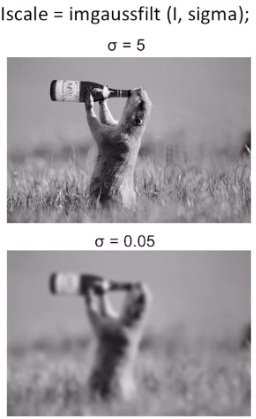
\includegraphics[scale=0.5]{1.png} 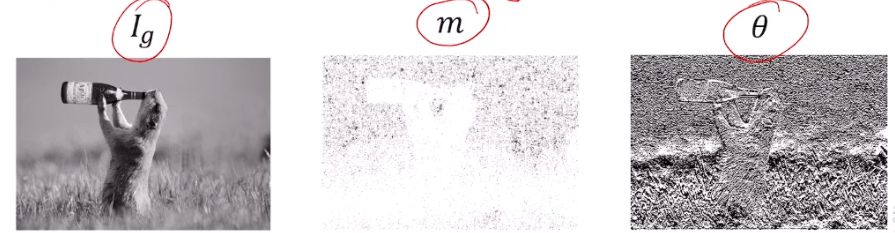
\includegraphics[scale=0.6]{2.png}
\end{center}
\begin{list}{}{}
	\item[4.] Create \textbf{gradient histogram}\begin{list}{}{}
		\item 4$\times$4 gradient window
		\item Histogram of 4$\times$4 per window on 8 orientation bins
		\item Gaussian weighting on center keypoint (width = $1.5\sigma$)
		\item 4$\times$4$\times$8 = 128 descriptor size
	\end{list}
\end{list}
\begin{center}
	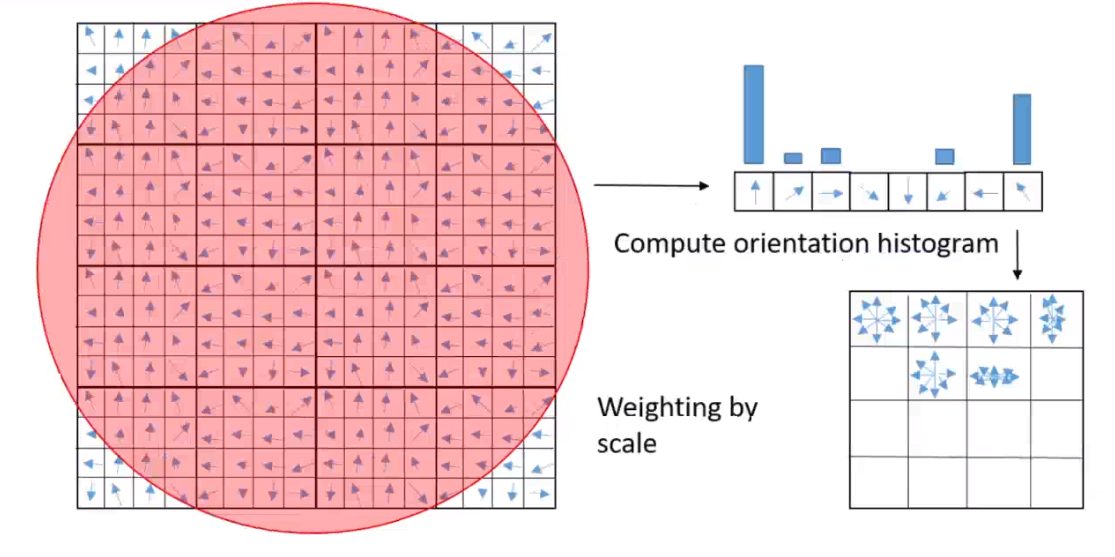
\includegraphics[scale=0.33]{3.png}
\end{center}
\paragraph{Fourier Analysis} Images are functions returning intensity values $I(x,y)$ on the 2D plane spanned by variables $x,y$. Not surprisingly, we can define the Fourier coefficients of a 2D-DFT as
$$H(k_x,k_y)=\sum_{x=1}^{N-1}\sum_{y=1}^{M-1}I(x,y)\cdot \exp\left(-2\pi i\left(\frac{xk_x}{N}\cdot\frac{yk_y}{M}\right)\right)$$
Basically, we can describe an image as a sum of $\sin$ and $\cos$ waves of varying frequency in $x$ and $y$ directions.
\paragraph{The Convolution Theorem} The Fourier transform $\mathbb{F}$ of the convolution of two functions is the product of their Fourier transforms
$$\mathbb{F}(f*g)=\mathbb{F}(f)\cdot\mathbb{F}(g)$$
Transforms convolutions in element-wise multiplications in Fourier domain. Suppose we have an Image $I$ (a function) and a filter $g$ (also a function): their convolution $I*g$ can be conveniently computed as
$$I*g = \mathbb{F}^{-1}(\mathbb{F}(I)\cdot\mathbb{F}(g))$$
with $\mathbb{F}^{-1}$ being the inverse Fourier transform.\\
Convolution is a very popular operation in deep learning, and the convolution theorem tells us that we can trade convolution on the spatial domain with multiplication on the spectral domain: we can implement convolutions efficiently and even compute convolution for non-standard signals (e.g.: graphs)\\
An issue with DFT on images is that is symmetric in both directions. The power spectrum is re-arranged to have the $(0,0)$ frequency (\textbf{DC component}) at the center of the plot: its magnitude is typically out-of-scale compared to other frequencies.
\subsubsection{Detectors}
\paragraph{Visual Feature Detector} Properties
\begin{list}{}{}
	\item \textbf{Repeatability} Detect the same feature in different image portions and different images, under different conditions (color, luminance\ldots). So with respect to translation, photometric changes, rotation, scaling and affine transformations (non-isotropic changes, for example the relative position of the camera)\ldots
\end{list}
\paragraph{Edge Detection} We need to find interesting points, talking about fundamental elements, basic components. One possible example are the edges of the image.\\
Reasoning in changes of intensity: edges are those points where the intensity changes.\begin{center}
	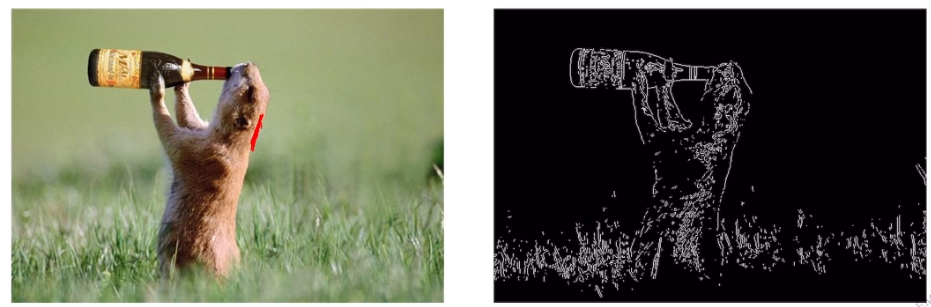
\includegraphics[scale=0.5]{4.png}
\end{center}
Typically using an edge detector filter on each pixel and turning pixels white or black by thresholding
\subparagraph{Edges and Gradients} The image gradient (graylevel) is $$\nabla I = \left[\frac{\partial I}{\partial x},\frac{\partial I}{\partial y}\right]$$ which is basically two images, gradient in both $x$ and $y$ directions. Edges are pixel regions where intensity gradient changes abruptly. The return of finite difference methods:
\begin{list}{}{}
	\item $G_x = \frac{\partial I}{\partial x} \simeq I(x+1,y)-I(x-1,y)$
	\item $G_y = \frac{\partial I}{\partial y} \simeq I(x,y+1)-I(x,y-1)$
\end{list}
Edge detectors build on this idea combining with some smoothing: average on multiple pixels.
\subparagraph{Prewitt operators}
$$G_x = \left[\begin{array}{c c c }
+1&0&-1\\
+1&0&-1\\
+1&0&-1
\end{array}\right]\:\:\:\:\:G_y = \left[\begin{array}{c c c }
+1&+1&+1\\
0&0&0\\
-1&-1&-1
\end{array}\right]$$
\begin{center}
	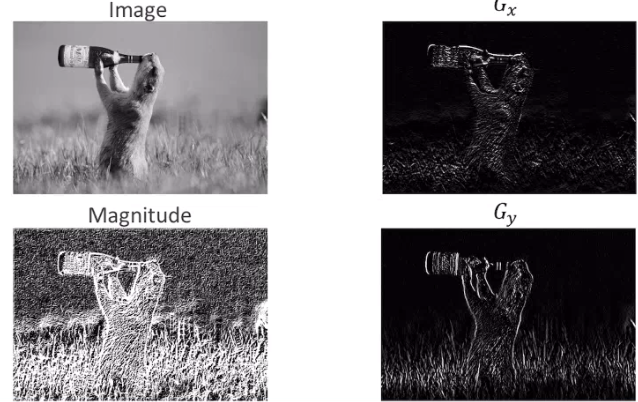
\includegraphics[scale=0.5]{5.png}
\end{center}
\subparagraph{Sobel Operator}
$$G_x = \left[\begin{array}{c c c }
+1&0&-1\\
+2&0&-2\\
+1&0&-1
\end{array}\right]\:\:\:\:\:G_y = \left[\begin{array}{c c c }
+1&+2&+1\\
0&0&0\\
-1&-2&-1
\end{array}\right]$$
Often with a constant $c\simeq \frac{1}{8}$ for scaling.
\begin{center}
	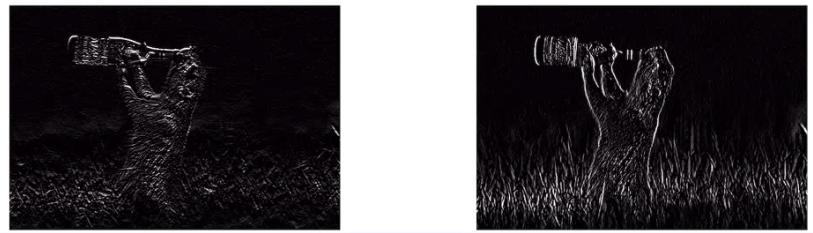
\includegraphics[scale=0.4]{6.png}
\end{center}
\paragraph{Blob Detection} Pixel regions with little gradient variability.\\
$g_\sigma(x,y)$ has maximum response when centered on a circle of radius $\sqrt{2}\sigma$, with $\sigma$ being the scale of the gaussian.\\
Laplace of Gaussian (LoG):
$$\nabla^2g_\sigma(x,y)=\frac{\partial^2g_\sigma}{\partial x^2} + \frac{\partial^2g_\sigma}{\partial y^2}$$
Typically using a scale normalized response
$$\nabla^2_{norm}g_\sigma(x,y)=\sigma^2\left(\frac{\partial^2g_\sigma}{\partial x^2} + \frac{\partial^2g_\sigma}{\partial y^2}\right)$$
\begin{enumerate}
	\item Convolve image with a LoG filter at different scales $\sigma = k\sigma_0$ by varying $k$ with a starting $\sigma_0$
	\item Find maxima of squared LoG responses:
	\begin{list}{}{}
		\item Find maxima on space-scale: focus on a scale and find maxima
		\item Find maxima between scales: do the same for all the scales and pick the maxima
		\item Threshold
	\end{list}
\end{enumerate}
The LoG can be approximated by the Difference of Gaussians (DoG) for efficiency, so to reuse part of the computations.
$$g_{k\sigma_0}(x,y) - g_{\sigma_0}(x,y) \simeq (k-1)\sigma_0^2\nabla^2g_{(k-1)\sigma_0}$$
SIFT uses LoG.
\paragraph{Affine Detectors} Laplacian-based detectors are invariant to scale thanks to the maximization in scale-space. Still not invariant to affine-transformation.
\begin{center}
	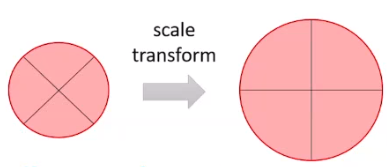
\includegraphics[scale=0.5]{7.png}\\
	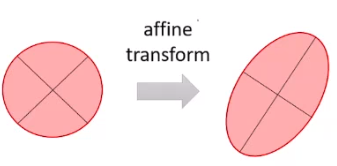
\includegraphics[scale=0.5]{8.png}
\end{center}
\paragraph{MSER} Maximally Stable Extremal Regions\\
Extract covariant regions (blobs) that are stable connected components of intensity sets of the image. Interesting areas stay the same at different thresholds: stable with respect to variations in luminance, not scale dependent and doesn't assume circular regions. The key idea is to \textbf{take the blobs} (\textbf{extremal regions}) \textbf{which are nearly the same through a wide range of intensity thresholds}.\\
Blobs are generated (locally) by binarizing the image over a large number of thresholds:\begin{list}{}{}
	\item Invariance to affine transformation of image intensities
	\item Stability (they are stable on multiple thresholds)
	\item Multi-scale (connected components are identified by intensity stability not by scale)
	\item Sensitive to local lightning effects, shadows\ldots
\end{list}
You can then fit an ellipse enclosing the stable region.
\subparagraph{Intuitions on MSER} Generate frames from the image by thresholding it on all graylevels.\\
Capture those regions that from a small seed of pixel grow to a stably connected region. Stability is assessed by looking at derivatives of region masks in time (most stable $\Rightarrow$ minima of connected region variation).
\paragraph{Image Segmentation} The process of partitioning an image into a set of homogeneous pixels, hoping to match objects or their subparts.\\
A naive approach: straighten the image in a $N\cdot M$ vector and use it as a dataset for K-means.\\
\subparagraph{Ncut} Normalized cuts
\begin{center}
	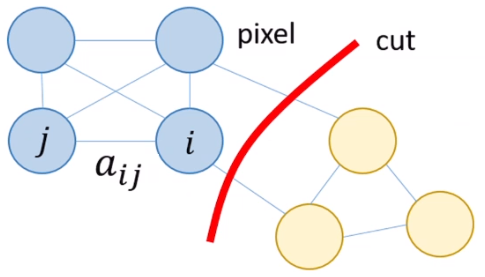
\includegraphics[scale=0.5]{9.png}
\end{center}
With each node being a pixel: an image is a graph. $a_{ij}$ is the affinity between pixels at a certain scale $\sigma$. A cut of $G$ is the set of edges such whose removal makes $G$ a disconnected graph. Breaking the graph into pieces by cutting edges of low affinity.\\
The normalized cut problem is NP-hard, approximate solution as an eigenvalue problem. But the eigenvalue decomposition it's really intractable with big images. We need to reduce the number of pixels. We can use \textbf{superpixels}: clustering the pixels with K-means (perhaps with different $K$) and using the clusters as nodes for segmentation algorithms (Ncut, Markov Random Fields\ldots). We can do multiscale superpixeling and segmenting at different scales, different policies\ldots
\subsubsection{Conclusion}
Image processing is a lot about convolutions: linear masks to perform gradient operations, gaussian functions to apply scale changes (zooming in and out). Computational efficiency is a driving factor: convolution in Fourier domain, superpixel, lightweight feature detectors\ldots
\subsection{Wavelets}
\paragraph{Limitations of DFT} Sometimes we might need localized frequencies rather than global frequency analysis.
\begin{center}
	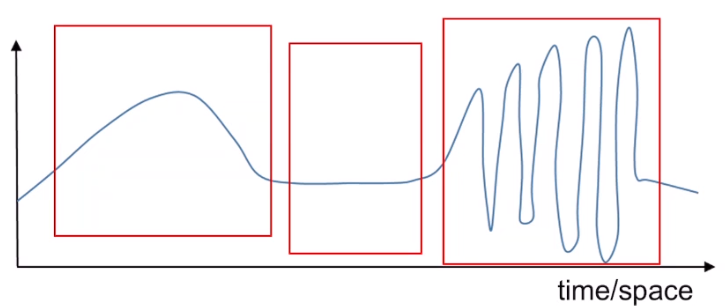
\includegraphics[scale=0.5]{10.png}
\end{center}
We slice the signal in "time slots" in time analysis and "frequency slots" in frequency analysis. In wavelet analysis you do both.\begin{center}
	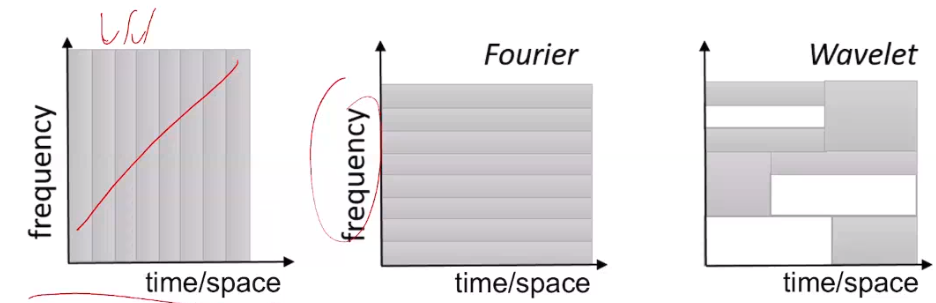
\includegraphics[scale=0.33]{11.png}\\
	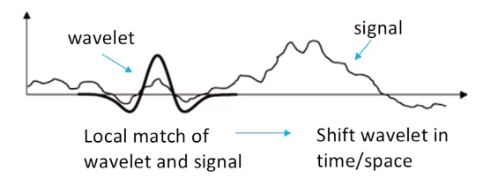
\includegraphics[scale=0.5]{12.png}
\end{center}
\begin{enumerate}
	\item Scale and shift original signal
	\item Compare signal to a wavelet
	\item Compute coefficient of similarity
\end{enumerate}
Split the signal with an orthonormal basis generate by translation and dilation of a mother wavelet $$\sum_t \mathbf{x}(t)\Psi_{j,k}(t)$$
Terms $k,j$ regulate scaling and shifting of the wavelet
$$\Psi_{j,k}(\mathbf{x}) = 2^{\frac{k}{2}}\Psi\left(\frac{t-j2^k}{2^k}\right) \simeq \frac{1}{\sqrt{j}}\Psi\left(\frac{t - k}{j}\right)$$
with respect to the mother wavelet $\Psi(\:)$: $k<1$ compresses the signal while $k>1$ dilates it.\\
Many different options for the mother wavelet $\Psi(\:)$
\begin{center}
	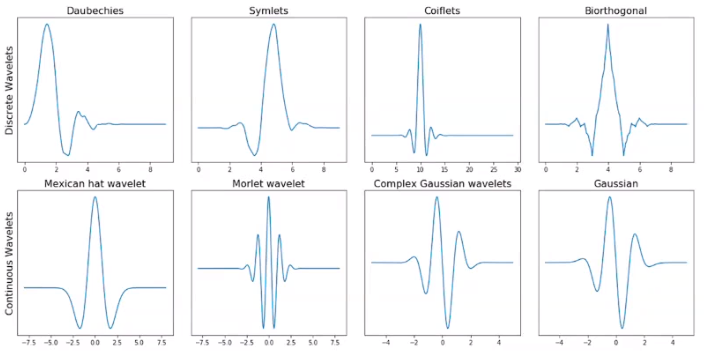
\includegraphics[scale=0.5]{13.png}
\end{center}
Scaling and dilation is akin to a sort of frequency: high scale mean stretched wavelet with slowly changing coarse feature and low frequency, while low scale compressed wavelet with rapidly changing details and high frequency.
\paragraph{DWT} Discrete Wavelet Transform: uses a finite set of scales and shifts rather than "any possible value" as in the continuous wavelet transform.

\section{Generative and Graphical Models}
These models \textbf{learn probabilities} and are \textbf{represented graphically}.
\begin{list}{}{}
	\item Generative refers to the the fact that we learn probabilities: if we know the distribution probability of data we can generate new data
	\item Graphical refers to the graphical formalisms that describe in a syntetic way the dependencies and influences
\end{list}
\paragraph{Generative Learning} ML \textbf{models that represent knowledge inferred from data under the form of probabilities}:
\begin{list}{}{}
	\item Probabilities can be sampled, so that new data can be generated
	\item Supervised, unsupervised or weakly supervised learning tasks
	\item More easily incorporate prior knowledge on data and tasks
	\item Interpretable knowledge (how data is generated)
\end{list}
Most modern tasks are composed by a large number of variables
\begin{list}{}{}
	\item Modeling the joint distribution of all variables can become impractical
	\item Exponential size of the parameter space
	\item Computationally impractical to train and predict
\end{list}
\paragraph{The Graphical Models Framework}
\begin{list}{}{}
	\item \textbf{Representation} Graphical models are a compact way to represent exponentially large probability distributions: we can encode conditional independence assumptions, and different classes of graph structures imply different assumptions/capabilities.
	\item \textbf{Inference} How to query (predict with) a graphical model? Probability of unknown $X$ given observations $\mathbf{d}$, $P(X\:|\:\mathbf{d})$, the \textbf{most likely hypothesis} (parameters) $X$.
	\item \textbf{Learning} Find the right model parameters.
\end{list}
\paragraph{Representation} A graph whose \textbf{nodes are random variables} and \textbf{edges represent probabilistic relationships} between the variables.\\
Different classes of graphs:
\begin{list}{}{}
	\item Directed edges express \textbf{causal relationships}.
	\item Undirected edges express \textbf{soft constraints}, values cannot change independently.
	\item \textbf{Dynamic models}, graphs subject to structure changes to reflect dynamic processes. For example RNNs: recurrent neural networks are unfolded using weight sharing, producing a dynamic model.
\end{list}
\paragraph{In Deep Learning} Bayesian learning necessary to understand Variational Deep Learning.
\begin{center}
	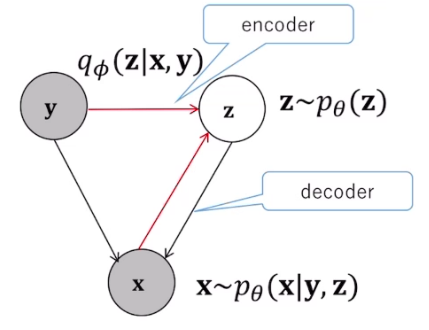
\includegraphics[scale=0.5]{14.png}
\end{center}
\paragraph{Generate new knowledge} Complex data can be generated if the model is powerful enough to capture its distribution.
\subsection{Probability Refresher}
\texttt{todo sorry in the mean time refer to other courses or online}
\subsubsection{Inference and Learning in Probabilistic Models}
\paragraph{Inference} How to determine the distribution of the values of one or more random variables, given the observed values of other random variables?
$$P(\text{graduate}\:|\:\text{exam}_1,\ldots,\text{exam}_n)$$
From a \textbf{machine learning point of view}: given a set of observations $\mathbf{d}$ and a set of hypothesis $\{h_i\}_i^K=1$, how can I use them to predict the distribution of a random variable $X$?
\paragraph{Learning} Learning is a \textbf{very specific inference problem}: given a set of observations $\mathbf{d}$ and a probabilistic model of a given structure, how do I find the parameters $\theta$ of its distribution? Amounts to \textbf{determining the best hypothesis $h_\theta$ regulated by a set of parameters $\theta$}.
\paragraph{Three Approaches to Inference}
\begin{list}{}{}
	\item \textbf{MAP} (Maximum a Posteriori): infer $X$ from $P(X\:|\:h_{MAP})$ where $h_{MAP}$ is the maximum a-posteriori hypothesys given $\mathbf{d}$
$$h_{MAP} = \arg\max_{h\in H} P(h\:|\:\mathbf{d}) = \arg\max_{h\in H}\underbrace{ P(\mathbf{d}\:|\:h)P(h)}$$
There are two distributions multiplied together, so they need to be coherent.
	\item \textbf{ML} (Maximum Likelihood): assuming uniform prioris $P(h_i)=P(h_j)$ yields the maximum likelihood estimate $P(X\:|\:h_{ML})$ $$h_{ML} = \arg\max_{h\in H} P(\mathbf{d}\:|\:h)$$
Any probability can be obtained from the Joint Probability Distribution $P(X_1,\ldots,X_n)$ by marginalization but at an exponential cost (e.g. $2^{n-1}$ for a marginal distribution from binary RV)
	\item \textbf{Bayesian}: consider all hypothesis weighted by their probabilities
$$P(X\:|\:\mathbf{d})=\sum_i P(X\:|\:h_i)P(h_i\:|\:\mathbf{d})$$
Optimal but poses computational and analytical tractability issues
$$P(X\:|\:\mathbf{d}) = \int_H P(X\:|\:h)P(h\:|\:\mathbf{d})\:dh$$
	ML and MAP are point estimates of the Bayesian, since they infer based only on one most likely hypothesis. MAP and Bayesian predictions become closer as more data gets available.\\
	MAP is a regularization of the ML estimation.
\end{list}
\paragraph{Regularization} Computing $P(h)$ introduces \textbf{preference across hypothesis}, penalizes complexity: complex hypothesis have lower prior probability, and hypothesis prior embodies trade-off between complexity and degree of fit.
The MAP hypothesis $h_{MAP}$ can be rearranged in a minimization problem with $\log_2$ (so to count the number of bits).
$$\max_h P(\mathbf{d}\:|\:h)P(h)\Leftrightarrow\min_h\underbrace{-\overset{\text{Bits needed for the data}}{\overbrace{\log_2(P(\mathbf{d}\:|\:h))}}-\overset{\text{Model complexity}}{\overbrace{\log_2P(h)}}}$$
The highlighted part is the number of bits needed to represent the data and the number of bits needed to represent the hypothesis. By optimizing only based on $\log_2(P(\underset{\uparrow}{\mathbf{d}}\:|\:h))$ we choose the hypothesis $h$ that best fits the data, potentially leading to overfitting. With the other term, $\log_2P(h)$, we penalize big models.
\paragraph{Maximum-Likelihood Learning} Find the model $\theta$ that is \textbf{most likely to have generated} the data $\mathbf{d}$ from a family of parameterized distributions $P(x\:|\:\theta)$
$$\theta_{ML} = \arg\max_{\theta\in \Theta} P(\mathbf{d}\:|\:\theta)$$
Optimization problem that considers the likelihood function $L(\theta\:|\:x)=P(x\:|\:\theta)$
as a function of $\theta$, which can be solved with $$\frac{\partial L(\theta\:|\:x)}{\partial\theta}=0$$
The \textbf{learning assumes that all random variables $X$ are visible}, as in Naive Bayes.\\
If the probabilistic model contains both observed random variables $\mathbf{X}$ (i.e. training data) and unobserved (also called hidden or latent) variables $\mathbf{Z}$ (e.g. data clusters), the ML learning can still be used to estimate model parameters:
\begin{list}{}{}
	\item Expectation-Maximization algorithm optimizes the complete likelihood
	$$L_c(\theta\:|\:\mathbf{X},\mathbf{Z})=P(\mathbf{X},\mathbf{Z}\:|\:\theta) = P(\mathbf{Z}\:|\:\mathbf{X},\theta)P(\mathbf{X}\:|\:\theta)$$
	\item A 2-step iterative process
	$$\theta^{(k+1)} = \arg\max_\theta\sum_{\mathbf{z}}P(\mathbf{Z}=\mathbf{z}\:|\:\mathbf{X},\theta^{(k)})\log(L_c(\theta\:|\:\mathbf{X},\mathbf{Z}=\mathbf{z})$$
\end{list}
\subsection{Graphical Models}
Compact graphical representation for exponentially large joint distributions: simplifies marginalization and inference algorithms, allowing to \textbf{incorporate prior knowledge} concerning causal relationships and associations between random variables.\begin{list}{}{}
	\item Directed graphical models (Bayesian Networks)
	\item Undirected graphical models (Markov Random Fields)
\end{list}
\subsubsection{Bayesian Networks} 
\begin{multicols}{2}
Directed Acyclic Graphs (DAG) $G = (V,E)$\begin{list}{}{}
	\item Nodes $v\in V$ represent random variables\\
	Shaded $\Rightarrow$ observed\\
	Empty $\Rightarrow$ unobserved (e.g. $Y_3$)
	\item Edges $e\in E$ describe the conditional independence relationships
\end{list}
\columnbreak
\begin{center}
	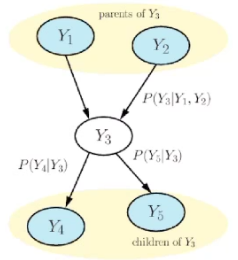
\includegraphics[scale=0.5]{15.png}
\end{center}
\end{multicols}
\paragraph{Conditional Probability Tables} CPTs are local to each node and describe the probability distribution \textbf{given its parents}.
$$P(Y_1,\ldots,Y_n) = \prod_{i=1}^N P(Y_i\:|\:\text{Parents}(Y_i))$$
\paragraph{Plate notation} If the same causal relationship is replicated for a number of variables, we can compactly represent it with plate notation.
$$P(Y_1,\ldots,Y_N,C) = P(C)\prod_{i=1}^N P(Y_i\:|\:C)$$
\begin{center}
	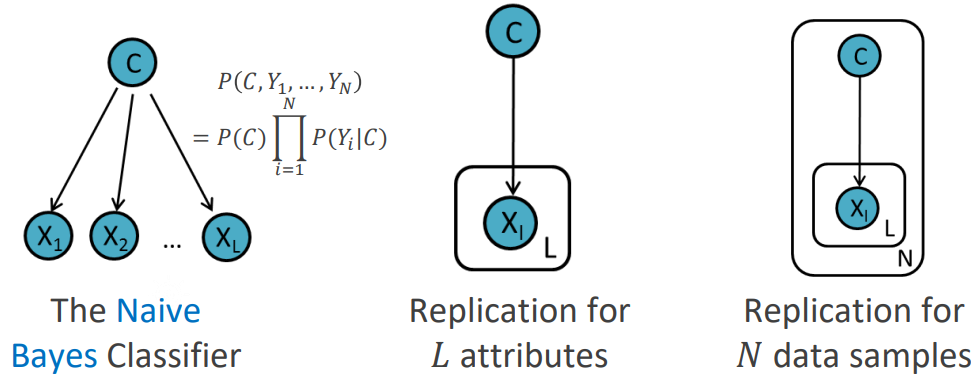
\includegraphics[scale=0.5]{16.png}
\end{center}
\pagebreak
\paragraph{Full-Plate Notation}
\begin{multicols}{2}
\begin{list}{}{}
	\item Boxes denote replication for a number of times (denoted by the letter in the corner)
	\item Shaded nodes are observed variables
	\item Empty nodes are unobserved latent variables.
	\item Black dots (optional) identify model parameters.
	\begin{list}{}{}
		\item $\pi$: multinomial prior distribution
		\item $\mu$, $\sigma$: mean and std. dev. of the Gaussian $C$
	\end{list}
\end{list}
\columnbreak
\begin{center}
	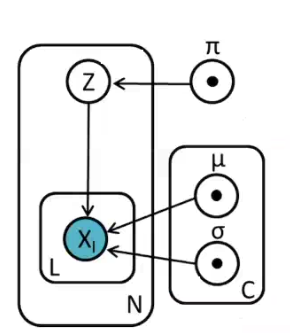
\includegraphics[scale=0.6]{17.png}
\end{center}
\end{multicols}
\subsubsection{Markov Random Fields}
\begin{center}
	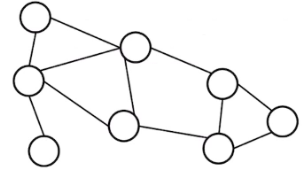
\includegraphics[scale=0.5]{18.png}
\end{center}
Undirected graphs $G = (V,E)$ (a.k.a. Markov Networks). Also with shaded/empty nodes to denote observed/unobserved variables.
\begin{list}{}{}
	\item \textbf{Nodes} $v\in V$ represent \textbf{random variables} $X_v$, with the shaded node meaning that it's \textbf{observed} and empty node meaning that it's \textbf{unobserved}.
	\item \textbf{Edges} $e\in E$ represent \textbf{bidirectional dependencies} between variables (\textbf{constraints})
\end{list}
Usually arranged in a structure that is coherent with the data/constraint we want to model.\\
Often used in image processing to impose spatial constraints (e.g. smoothness)
\subsection{Conditional Independence and Causality}
Can we reason on the structure of the graph to infer direct/indirect relationships between random variables?
\paragraph{Local Markov Property} Each node (random variable) is conditionally independent of all its non-descendants given a joint state of its parents. $$\forall\:v\in V\:\:Y_v\perp Y_{V\setminus \text{Children(v)}}\:|\:Y_{\text{Parent}(v)}$$
To be read as "$Y_v$ is independent from all the RVs in $Y$ that are not children of $v$ given the parents of $v$".\\
There are substructures in the Bayesian networks with which we can build everything.
\paragraph{Markov Blanket} A Markov blanket $Mb(A)$ of a node $A$ is the minimal set of vertices that isolates/shields the node from the rest of the Bayesian network. If I know the variables in $Mb(A)$ then I know everything I need to know about $A$\begin{center}
	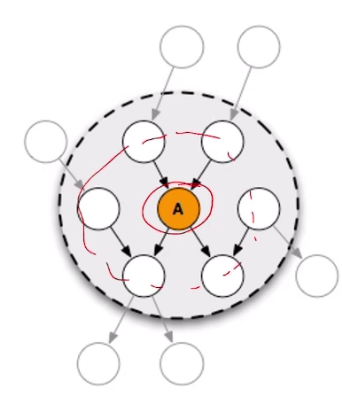
\includegraphics[scale=0.33]{19.png}
\end{center}
Taking only the parents it's not sufficient, we need also the children and the co-parents (nodes that are parents of one of my children). So it contains parents, children and children's parents.
$$P(A\:|\:Mb(A), Z) = P(A\:|\:Mb(A))\:\:\forall\:Z\not\in Mb(A)$$
\pagebreak
\paragraph{Joint Probability Factorization}
\begin{multicols}{2}
An application of the chain rule and local Markov property.\begin{enumerate}
	\item Pick a topological ordering of the nodes
	\item Apply chain rule following the order
	\item Use the conditional independence assumptions
\end{enumerate}
\columnbreak
\begin{center}
	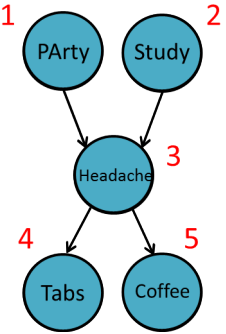
\includegraphics[scale=0.5]{209.png}
\end{center}
\end{multicols}
$$P(PA,S,H,T,C) = P(PA)\cdot P(S\:|\:PA)\cdot P(H\:|\:S,PA)\cdot P(T\:|\:H,S,PA)\cdot P(C\:|\:T,H,S,PA)=$$
$$=P(PA)\cdot P(S)\cdot P(H\:|\:S,PA)\cdot P(T\:|\:H)\cdot P(C\:|\:H)$$
\paragraph{Sampling of a Bayesian Network} A BN describes a generative process for observations.
\begin{enumerate}
	\item Pick a topological ordering of the nodes
	\item Generate data by sampling from the local condition probabilities following this order
\end{enumerate}
Generate $i$th sample for each variable, example $s_i\sim P(S)$, $pa_i\sim P(PA)$, $h_i\sim P(H\:|\:S=s_i, PA = pa_i)$
\subsection{Fundamental Bayesian Network Structures}
Three fundamental substructures that determine the conditional independence relationships in a Bayesian network.
\paragraph{Tail to Tail} Common cause \begin{center}
	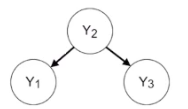
\includegraphics[scale=0.75]{20.png}
\end{center}
$$P(Y_1,Y_3\:|\:Y_2)=P(Y_1\:|\:Y_2)P(Y_3\:|\:Y_2)$$
If $Y_2$ is unobserved, then $Y_1,Y_3$ are marginally dependent $Y_1\not\perp Y_3$\\
If $Y_2$ is observed, $Y_1,Y_3$ become conditionally independent $Y_1\perp Y_3\:|\:Y_2$ (the path between $Y_1,Y_3$ is blocked by the observed (shaded) $Y_2$)
\paragraph{Head to Tail} Causal Effect \begin{center}
	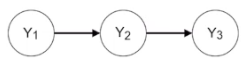
\includegraphics[scale=0.75]{21.png}
\end{center}
$$P(Y_1,Y_3\:|\:Y_2)=P(Y_1)P(Y_2\:|\:Y_1)P(Y_3\:|\:Y_2)=P(Y_1\:|\:Y_2)P(Y_3\:|\:Y_2)$$
Same behavior as before!\\
If $Y_2$ is unobserved, then $Y_1,Y_3$ are marginally dependent $Y_1\not\perp Y_3$\\
If $Y_2$ is observed, $Y_1,Y_3$ become conditionally independent $Y_1\perp Y_3\:|\:Y_2$ ($Y_2$ again blocks the path)
\paragraph{Heat to Head} Common effect\begin{center}
	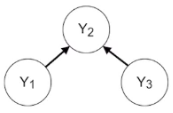
\includegraphics[scale=0.75]{22.png}
\end{center}
$$P(Y_1,Y_2,Y_3) = P(Y_1)P(Y_3)P(Y_2\:|\:Y_1,Y_3)$$
If $Y_2$ is unobserved, then $Y_1,Y_3$ are marginally independent $Y_1\perp Y_3$\\
If $Y_2$ is observed, then $Y_1,Y_3$ are conditionally dependent $Y_1\not\perp Y_3\:|\:Y_2$\\
If any $Y_2$ descendants is observed it unlocks the path.
\paragraph{Derived Conditional Independence Relationships} A Bayesian network represent the local relationship encoded by the 3 basic structures plus the derived relationships.\\\\
Given the same distribution I can have two different Bayesian Networks, which implies the same factorization.
\begin{center}
	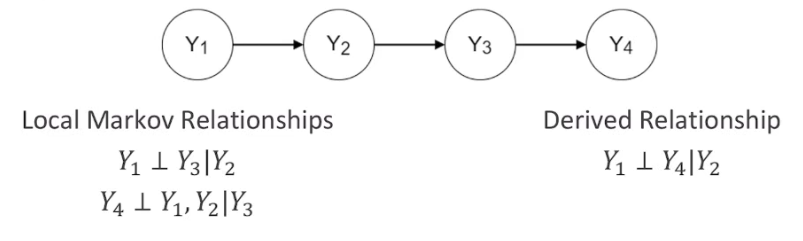
\includegraphics[scale=0.5]{23.png}
\end{center}
\paragraph{$d$-separation} Let $r = Y_1\leftrightarrow\ldots\leftrightarrow Y_2$ be an undirected path between $Y_1,Y_2$, $r$ is $d$-separated by $Z$ if there exist at least one node $Y_c\in Z$ for which path $r$ is blocked. With $Z$ being the set of variables for which we're assessing this separation.\\
In other words, this holds if at least one of the following holds:\begin{list}{}{}
	\item $r$ contains an head-to-tail structure $Y_i\rightarrow Y_c\rightarrow Y_j$ (or $Y_i\leftarrow Y_c\leftarrow Y_j$) and $Y_c \in Z$
	\item $r$ contains a tail-to-tail $Y_i\leftarrow Y_c\rightarrow Y_j$ and $Y_c \in Z$
	\item $r$ contains head-to-head $Y_i\rightarrow Y_c\leftarrow Y_j$ and neither $Y_c$ nor its descendants are in $Z$
\end{list}
Two nodes $Y_i,Y_j$ in a Bayesian Network $G$ are $d$-separated by $Z\subset V$ $\Leftrightarrow$ all undirected paths between $Y_i,Y_j$ are $d$-separated by $Z$ (denoted by $\text{Dsep}_G(Y_i,Y_j\:|\:Z)$)
\paragraph{Markov Blanket} The Markov Blanket $Mb(Y)$ is the minimal set of nodes which $d$-separates a node $Y$ from all other nodes (i.e. makes $Y$ conditionally independent of all other nodes in the Bayesian Network)
$$Mb(Y) = \{\text{Parents}(Y), \text{Children}(Y), \text{Parents}(\text{Children}(Y))\}$$
\paragraph{Are Directed Models Enough?} Bayesian Networks are used to model asymmetric dependencies. But \textbf{directed models cannot express all conditional dependence relationships}: expressing some precludes the expressions of others.\\
What if we want to model symmetric dependencies, like bidirectional effects, spatial dependencies\ldots Directed models cannot represent some bidirectional dependencies in the distributions. We need \textbf{undirected approaches}.
\subsection{Markov Random Fields}\begin{center}
	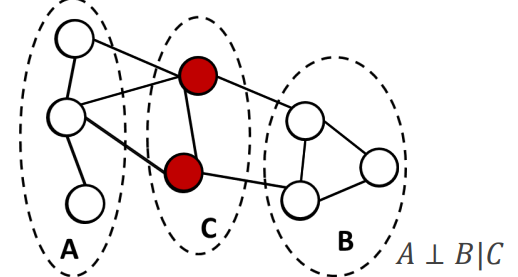
\includegraphics[scale=0.5]{24.png}
\end{center}
What is the undirected equivalent of $d$-separation in directed models? It's based on node separation: the two nodes in the middle separate the two lateral parts.\\
Node subsets $A,B\subset V$ are conditionally independent given $C\subset V\setminus \{A,B\}$ if all paths between nodes in $A$ and $B$ pass through at least one of the nodes in $C$.\\
The Markov Blanket of a node includes all and only its neighbors.
\paragraph{Joint Probability Factorization} What is the undirected equivalent? We seek a product of functions defined over a set of nodes associated with some local properties of the graph. Markov blanket tells that nodes that are not neighbors are conditionally independent given the rest of the nodes.$$P(X_v,X_i\:|\:X_{V\setminus\{v,i\}}) = P(X_v\:|\:X_{V\setminus\{v,i\}})P(X_i\:|\:X_{V\setminus\{v,i\}})$$
Factorization should be chosen in a way that nodes $X_v$ and $X_i$ are not in the same factor: we use a well-known graph structure that includes only nodes that are pairwise connected.
\subparagraph{Clique} Subset of nodes $C$ in graph $G$ such that $G$ contains an edge between all pair of nodes in $C$. It's maximal if you cannot add more nodes.
\begin{center}
	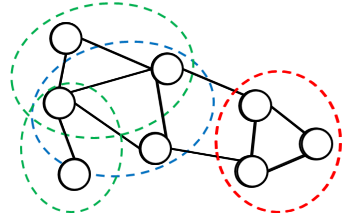
\includegraphics[scale=0.5]{210.png}
\end{center}
\subparagraph{Maximal Clique Factorization} Define $X = X_1,\ldots,X_n$ as the random variables associated to the $N$ nodes of the undirected graph $G$ $$P(X)=\frac{1}{Z}\prod_C \psi(X_C)$$
$X_C$ are the random variables in the maximal clique $C$, $\psi(X_C)$ is the \textbf{potential function} over the maximal clique $C$ and $Z$ is the partition function ensuring normalization.
$$Z = \sum_X\prod_C\psi(X_C)$$
The partition function $Z$ is the computational bottleneck of undirected models: $O(K^N)$ for $N$ discrete random variables with $K$ distinct values.
\paragraph{Potential Functions} It's important to state how \textbf{potential functions} $\psi(X_C)$ \textbf{are not probabilities}: they express which configuration of the local variables are preferred. They can be seen as hand-engineered feature functions. An example of potential function is $$\psi(X_1,X_2)=\left\{ \begin{array}{l l}
1&\text{if }X_1 = X_2\\
4&\text{if }X_2 = 2X_1\\
0&\text{otherwise}
\end{array}\right.$$
If we restrict to strictly positive potential functions, the Hammersley-Clifford theorem provides guarantees on the distribution that can be represented by the clique factorization.
\subparagraph{Boltzmann Distribution} A widely used strictly positive representation of the potential function is $$\psi(X_C)=e^{-E(X_C)} = e^{\frac{X_C}{kT}}$$
where $E(X_C)=-\frac{\displaystyle X_C}{\displaystyle kT}$ is called \textbf{energy function}.
\subsubsection{From Directed to Undirected}
Straightforward when is linear.\\Requires some work with v-structures, e.g. \textbf{moralization} (a.k.a. marrying of the parents).\begin{center}
	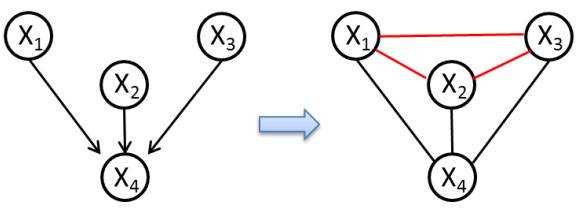
\includegraphics[scale=0.5]{25.png}
\end{center}
\pagebreak
\subsection{Learning Causation from Data}
\paragraph{Learning with Bayesian Network}
\begin{center}
	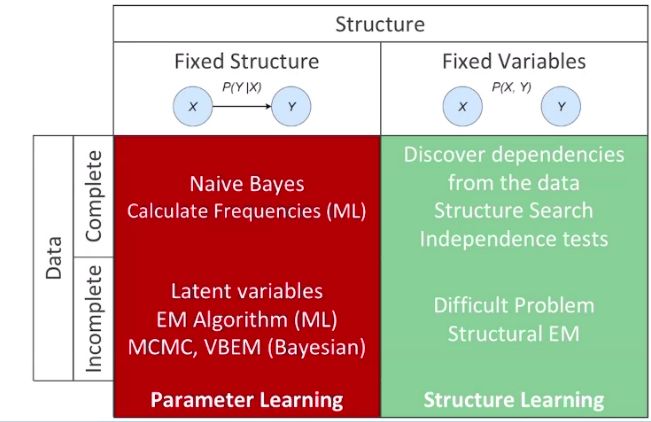
\includegraphics[scale=0.33]{26.png}
\end{center}
\paragraph{Structure Learning Problem} Observations are given for a set of fixed random variables, and network structure is not specified:\begin{list}{}{}
	\item \textbf{Determine which arcs exist} in the network (causal relationships)
	\item \textbf{Compute Bayesian network parameters} (conditional probability tables)
\end{list}
Determining causal relationships between variables entails deciding on arc presence and directing edges.
\subparagraph{Structure Finding Approaches}\begin{list}{}{}
	\item \textbf{Search and Score}\\A model selection approach, a search in the space of the graphs.\\
	Search the space Graph$(Y)$ of graphs $G_k$ that can be built on the random variables $Y = Y_1,\ldots,Y_N$, scoring each structure by $S(G_k)$ and returning the highest scoring graph $G^*$.\\Two fundamental aspects: the \textbf{scoring function} and the \textbf{search strategy}.
	\begin{multicols}{2}
	The \textbf{scoring function} must have two fundamental properties:\begin{list}{}{}
		\item \textbf{Consistency}: same score for graphs in the same equivalence class
		\item \textbf{Decomposability}: can be locally computed
	\end{list}
	Two main approaches\begin{list}{}{}
		\item \textbf{Information theoretic}: based on data likelihood plus some model-complexity penalization terms
		\item \textbf{Bayesian}: score the structures using a graph posterior (likelihood plus proper prior choice)
	\end{list}
	\columnbreak
	As for the \textbf{search strategy}, finding maximal scoring structures is NP complete.\\
	\textbf{Constrain search strategy}: starting from a candidate structure we modify iteratively by local operations (edge/node addition/deletion), and each operation has a cost so this is a cost optimization problem. The constraint search space can be\begin{list}{}{}
		\item Known node order: can reduce the search space to the parents of each node (Markov Blankets)
		\item Search in the space of structure equivalence classes
		\item Search in the space of node ordering
	\end{list}
	\end{multicols}
	\item \textbf{Constraint Based}\\
	Tests of conditional independence $I(X_i,X_j\:|\:Z)$, constraining the network. Based on measures of association between two variables $X_i$ and $X_j$ given their neighbor nodes $Z$ and using deterministic rules based on local Markovian dependencies to determine edge orientation (DAG).\\
	In the \textbf{testing strategy}, the choice of the testing order is fundamental in avoiding a super-exponential complexity:\begin{list}{}{}
		\item \textbf{Level-wise testing}: tests $I(X_i,X_j\:|\:Z)$ are performed in order of increasing size of the conditioning set $Z$ starting from $Z = \emptyset$ (PC algorithm)
		\item \textbf{Node-wise testing}: tests are performed on a single edge at the time, exhausting independence checks on all conditioning variables (TPDA algorithm)
	\end{list}
	The nodes entering $Z$ are chosen in the neighborhood of $X_i,X_j$
	\item \textbf{Hybrid}\\
	Model selection of constrained structures. Multi-stage algorithms combining previous approaches: independence tests to find a good sub-optimal skeleton as starting point, then search and score refining the skeleton.\\
	Max-Min Hill Climbing (MMHC) model: optimized constraint-based approach to reconstruct the skeleton, using the candidate parents in the skeleton to run a search and score approach.
\end{list}
\paragraph{PC Algorithm} Expressed by the following pseudocode
\begin{lstlisting}
Initialize a fully connected graph G = (V, E)
for each edge (Yi, Yj) in V
	if I(Yi, Yj) then Prune((Yi, Yj))
K = 1
for each test of order K == |Z|
	for each edge (Yi, Yj) in V
		Z = set of conditioning sets of Kth order for Yi, Yj
		if I(Yi, Yj | z) for any z in Z then Prune((Yi, Yj))
	K = K + 1
return G
\end{lstlisting}
%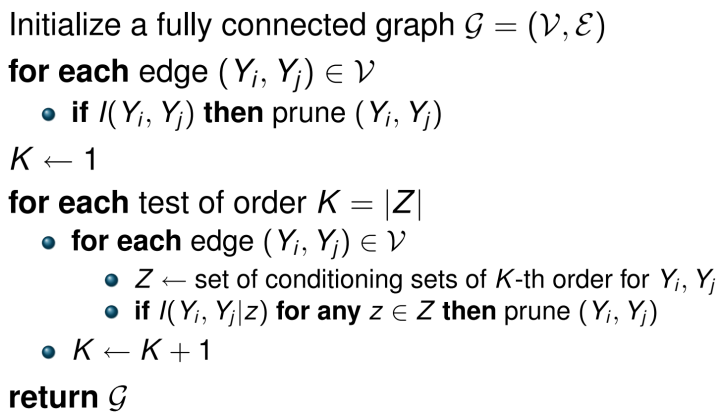
\includegraphics[scale=0.5]{211.png}
\subsection{Hidden Markov Models}
\paragraph{Sequence} A sequence $y$ is a \textbf{collection of observations} $y_t$, where $t$ represents the position of the element according to a complete order (e.g. time)
$$y_1\rightarrow \ldots\rightarrow y_{t-1}\rightarrow y_t\rightarrow\ldots\rightarrow y_T$$
$$P(y_t\:|\:y_{t-1})$$
Also head-to-tail: observation at time $t$ is independent from $t=1,\ldots,t-1$ (\textbf{first-order Markov assumption}).\\
Reference population is a set of independent and identically distributed sequences $y^1, \ldots, y^N$\\
Difference sequences $y^1, \ldots, y^N$ generally have different lengths $T^1,\ldots,T^N$
\paragraph{Markov Chain} First-Order Markov Chain is a directed graphical model for sequences such that element $x_t$ only depends on the previous node $x_{t-1}$.\\
We have X = $x_1,\ldots,x_T$ that can be represented as 
$$x_1\rightarrow \ldots\rightarrow x_{t-1}\rightarrow x_t\rightarrow\ldots\rightarrow x_T$$
So we can write $$P(\text{X}) = P(x_1,\ldots,x_T) = P(x_1)\cdot\prod_{i=2}^T P(x_i\:|\:x_{i-1})$$
and, due to \textbf{stationarity}, $P(x_i\:|\:x_{i-1})$ is the same for each $i$.\\
$P(x_1)$ is the \textbf{prior distribution} ($x_1$ has nothing "before" it) and $P(x_i\:|\:x_{i-1})$ is the \textbf{transition distribution}.
\subparagraph{Example} Assuming $x_t\in\{a,\ldots,z\}$, so of 25 elements, this gives $P(x_1) = P(x_1 =$ letter$)$ so $P(x_1)$ is a vector with each position being the probability of $x_1$ being that letter. Summing the vector elements gives 1, because it's a distribution of probabilities. This makes $P(x_i\:|\:x_{i-1})$ a matrix of 25$\times$25 elements: in position $(n,b)$ there is $P(x_i=n\:|\:x_{i-1}=b)$. The sum of the elements in a single column will be $1$ (sum-to-one), because the conditional probability gives a family of distribution: for each assignment there is a distribution.\\\\
The general form is the $L$th order Markov chain, when $x_i$ depends on $L$ predecessors.
\paragraph{Observed Markov Chains} We can use the Markov chain to model the relationships between observed elements in a sequence. The problem is that we can do that only pairwise: computational issue (very large matrices) and e.g. only co-occurrence of 2 words so unapplicable to natural language.\\
So we need to \textbf{abstract from symbols to category}: not relationship between words, but relationships between the general concepts represented by those words. The \textbf{categories are not observable}: Markov chain over non-observable elements.
\paragraph{Hidden Markov Models} An HMM infers categories: stochastic process where transition dynamics is disentangled from observations generated by the process.\begin{center}
	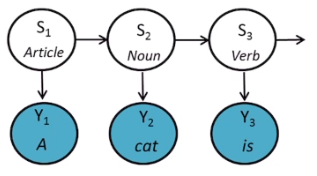
\includegraphics[scale=0.5]{27.png}
\end{center}
$S_i$ are \textbf{hidden states}, finite ($i = 1,\ldots,C$). We need \textbf{clustering algorithms}: clustering symbols into a finite set of non-observable elements. The main elements are:
\begin{list}{}{}
	\item Multinomial \textbf{state transition} $A_{ij} = P(S_t=i\:|\:S_{t-1}=j)$
	\item \textbf{Prior probability} (stationary assumption) $\pi_i = P(S_1=i)$
	\item \textbf{Emission distribution} (the "down arrow" $\begin{array}{c}
S_t\\\downarrow\\Y_t
\end{array}$) $b_i(y_t) = P(Y_t = y_t\:|\:S_t = i)$
\end{list}
\paragraph{HMM Joint Probability Factorization} Discrete state HMMs are parameterized by the finite number of hidden states $C$ and $\Theta = (\pi, A, B)$:
\begin{list}{}{}
	\item $\pi$ prior distribution
	\item $A$ state transition
	\item $B$ emission distribution (or its parameters)
\end{list}
$$P(Y = y) = \sum_s P(Y=y,S=s) =$$
$$= \sum_{s_1,\ldots,s_T}\left( P(S_1=s_1)P(Y_1=y_1\:|\:S_1=s_1)\prod_{t=2}^T P(S_t=s_t\:|\:S_{t-1} = s_{t-1})P(Y_t=y_t\:|\:S_t=s_t)\right)$$
\paragraph{HMMs as Recursive Models} A graphical framework describing how contextual information is recursiverly encoded by both probabilistic and neural models.
\begin{center}
	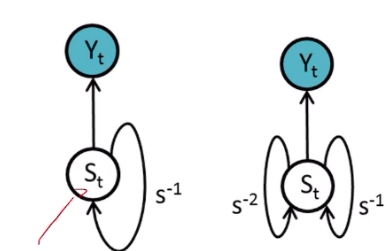
\includegraphics[scale=0.5]{28.png}
\end{center}
Indicates that the hidden state $S_t$ at time $t$ is dependent on context information from
\begin{list}{}{}
	\item the previous timestep $s^{-1}$, first-order
	\item the previous two timesteps $s^{-1},s^{-2}$, second-order
\end{list}
and so on. Applying the recursive model to a sequence (\textbf{unfolding}) generates the corresponding \textbf{directed graphical model}.
\paragraph{HMMs as Automata} Can also be generalized to transducers.
\begin{center}
	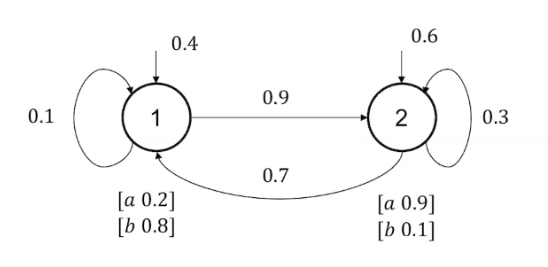
\includegraphics[scale=0.5]{29.png}
\end{center}
\subsection{Notable Inference Problems}
\paragraph{Smoothing} Given a model $\Theta$ and an observed sequence $y$, determine the distribution of the hidden state at time $t$: $P(S_t\:|\:Y=y,\Theta)$. (Forward Backward algorithm)
\paragraph{Learning} Given a dataset of $N$ sequences $D=\{y^1,\ldots,y^N\}$ and the number of hidden states $C$, find the parameters $\pi,A,B$ that maximize the probability model $\Theta = \{\pi,A,B\}$ having generated the sequences in $D$
\paragraph{Optimal State Assigment} Given a model $\Theta$ and an observed sequence $y$, find an optimal state assignment $s = s_1^*,\ldots,s_T^*$ for the hidden Markov chain. (Viterbi algorithm)
\subsubsection{Forward-Backward Algorithm} \textbf{Smoothing}: how do we determine $P(S_t = i\:|\:\hat{y})$? We will compute $P(S_t=i, \hat{y})$, it's proportional (just divide by $P(\hat{y})$). It's possible to directly estimate $P(S_t = i\:|\:\hat{y})$ (\textbf{smoothed posterior}), but it's more involved.\\
I know $\Theta=\{\pi,A,B\}$, the parameters of the model, thus I know 
\begin{list}{}{}
	\item The prior $\pi = P(S_1)$
	\item The transition probability $A = P(S_t\:|\:S_{t-1})$
	\item The emission probability $B = P(y_t\:|\:S_t)$
\end{list}
I need to express the quantity I want in terms of $\Theta$.\\\\
$\hat{y}$ are all the observations for each timestep $\Rightarrow P(S_t=i,y_1,\ldots,y_{t-1},y_t,y_{t+1},\ldots,y_T)$
$$\begin{array}{ccccccccccccc}
S_1&\rightarrow&\ldots&\rightarrow&S_{t-1}&\rightarrow&S_t&\rightarrow&S_{t+1}&\rightarrow&\ldots&\rightarrow&S_T\\
\downarrow& &\ldots& &\downarrow& &\downarrow& &\downarrow& &\ldots& &\downarrow\\
y_1&&\ldots&&y_{t-1}&&y_t&&y_{t+1}&&\ldots&\&y_T
\end{array}$$
We are at time $t$, so everything after that is the future ($y_{t+1:T}$), and everything up to $t$ included is the past ($y_{1:t}$).
$$P(S_t=i,y_1,\ldots,y_{t-1},y_t,y_{t+1},\ldots,y_T) = P(y_{t+1:T}\:|\:S_t=i, y_{1:t}) P(S_t=i,y_{1:t})=$$
By observing $S_t$ we block all the paths from the past $y_{1:t}$ to the future $y_{t+1:T}$, so $P(y_{t+1:T}\:|\:S_t=i, y_{1:t}) = P(y_{t+1:T}\:|\:S_t=i)$
$$P(S_t=i,y_1,\ldots,y_{t-1},y_t,y_{t+1},\ldots,y_T) = \underset{\beta_t(i)}{\underbrace{P(y_{t+1:T}\:|\:S_t=i)}} \underset{\alpha_t(i)}{\underbrace{P(S_t=i,y_{1:t})}}$$
I can derive two "messages"
\begin{list}{}{}
	\item \textbf{Past message} $\alpha_t(i) = P(S_t=i,y_{1:t})$: \textbf{forward recursion} with $\alpha_1(i)=b_i(y_1)\pi_i$
	\item \textbf{Future message} $\beta_t(i) = P(y_{t+1:T}\:|\:S_t=i)$: \textbf{backward recursion} with $\beta_T(i) = 1$ for every $i$
\end{list}
The past message can be written as follows, introducing $S_{t-1}$ by marginalization
$$\alpha_t(i) = P(S_t = i,y_{1:t}) = \sum_{j=1}^c P(S_t = i, S_{t-1}=j,y_{1:t}) = \sum_{j=1}^c P(y_t\:|\:S_t = i, S_{t-1} = j, y_{1:t-1})P(S_t = i,S_{t-1} = j,y_{1:t-1})$$
Which can be simplified like:
\begin{list}{}{}
	\item $P(y_t\:|\:S_t = i, \cancel{S_{t-1} = j}, \cancel{y_{1:t-1}}) = P(y_t\:|\:S_t=i)$\\
	Because we observe $S_t$ we can get rid of $S_{t-1}=j$ and $y_{1:t-1}$ leaving us with $P(y_t\:|\:S_t)$ which is just the emission
	\item $P(S_t = i,S_{t-1} = j,y_{1:t-1}) = P(S_t = i\:|\:S_{t-1}=j,\cancel{y_{1:t-1}}) \underset{\alpha_{t-1}(j)}{\underbrace{P (S_{t-1}=j, y_{1:t-1})}} = P(S_t = i\:|\:S_{t-1}=j)\alpha_{t-1}(j)$\\
	It can be rewritten and then, by observing $S_{t-1}$, we can get rid of $y_{1:t-1}$, giving us the transition distribution and $\alpha_{t-1}(j)$
\end{list}
$$\alpha_t(i) = P(S_t=i,y_{1:t}) = \sum_{j=1}^c P(y_t\:|\:S_t=i) P(S_t=i\:|\:S_{t-1}=j)\alpha_{t-1}(j)$$
$$\alpha_1(j) = P(y_1\:|\:S_1=j)P(S_1=j)$$
This just by reasoning with conditional independence.
\pagebreak

Same thing can be done for backward recursion introducing $S_{t+1}$ by marginalization $$\beta_t(i) = P(y_{t+1:T}\:|\:S_{t} = i) = \sum_j P(y_{t+1:T},S_{t+1}=j\:|\:S_t=i) = \sum_j P(y_{t+2:T}\:|\:S_t, S_{t+1},y_{t+1})P(S_{t+1},y_{t+1}\:|\:S_t=i)$$
Same as before
\begin{list}{}{}
	\item $P(y_{t+2:T}\:|\:\cancel{S_t}, S_{t+1},\cancel{y_{t+1}}) = \beta_{t+1}(j)$\\
	I can exclude $S_t, y_{t+1}$ because we observe $S_{t+1}$
	\item $P(S_{t+1},y_{t+1}\:|\:S_t=i) = P(S_{t+1}\:|\:S_t,\cancel{y_{t+1}})P(y_{t+1}\:|\:S_{t+1})$\\
	It is rewritten like such, which is the transition distribution times the emission distribution.
\end{list}
$$\beta_t(i) = \sum_j P(y_{t+1}\:|\:S_{t+1} = j)P(S_{t+1}=j\:|\:S_t=i)\beta_{t+1}(j)$$
$$\beta_T = 1$$
\paragraph{Sum-Product Message Passing} The Forward-Backward algorithm is an example of a sum-product message passing algorithm.\\
A forward recursion computing a generic message $\mu_\alpha$, backward recursion computing a generic message $\mu_\beta$\\
A general approach to efficiently perform exact inference in graphical models, with $\alpha_t \equiv \mu_\alpha(X_n)$ and $\beta_{t}\equiv \mu_\beta(X_n)$
$$\mu_\alpha(X_n) = \sum_{X_{n+1}} \psi(X_n, X_{n+1})\mu_\beta(X_{n+1})$$
\subsubsection{Learning in HMM}
Learning parameters $\Theta=(\pi,A,B)$ by \textbf{maximum} (log) \textbf{likelihood}
$$L(\Theta) = \log\prod_{n=1}^N P(Y^n\:|\:\Theta) = \log\prod_{n=1}^N\left(\sum_{S_1^n,\ldots,S_{T_n}^n} P(S_1^n)P(Y_1^n\:|\:S_1^n)\prod_{t=2}^T P(S_t^n\:|\:S_{t-1}^n)P(Y_t^n\:|\:S_t^n)\right)$$
Maximizing the joint likelihood of the sequences given the parameters considering them independent and identically distributed. We have to deal with the unobserved $S_t^n$ and the nasty sum in the log.\\
Expectation-Maximization of the \textbf{complete likelihood} $L_c(\Theta)$, optimizing a slightly different problem obtaining a not-reducing similar result. It's completed with indicator variables $z_{ti}^n=\left\{\begin{array}{c l}
1&\text{if }n\text{th chain is in state }i\text{ at time }t\\
0&\text{otherwise}
\end{array}\right.$ about the assignments $S_i^n$ (meaning $z_{ti}^n = 1\Leftrightarrow S_t = i$)
\paragraph{Expectation-Maximization} Gives the red line: touching in the estimating point and not greater in the other points.
\begin{center}
	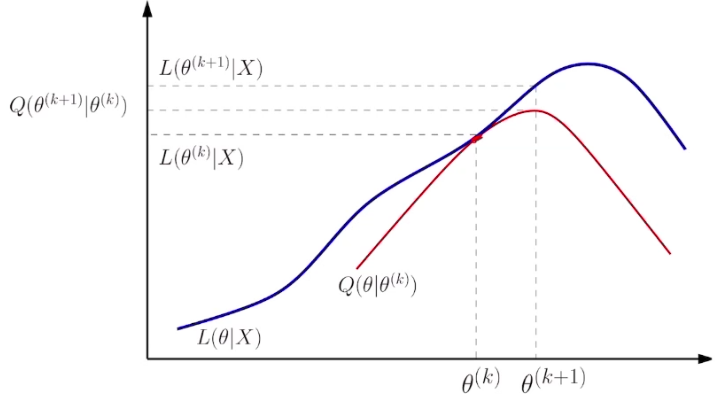
\includegraphics[scale=0.5]{30.png}
\end{center}
It's a matter of picking the right $Q(\Theta\:|\:\Theta^k)$\\
Introduce indicator variables in $L(\Theta)$ together with model parameters $\Theta = (\pi,A,B)$
\pagebreak
$$L_C(\Theta)=\log P(Y,Z\:|\:\Theta) = $$
$$ = \log\underset{\text{Sequences}}{\underbrace{\prod_{n=1}^N}}\left(\underset{=P(S_1=i^*)P(Y_1^n\:|\:S_1=i^*)}{\underbrace{\overset{\text{All }C\text{ terms are 1 except for the single }z_{1i^*}^n=1}{\overbrace{\underset{\text{Assignments}}{\underbrace{\prod_{i=1}^C}} \left(\underset{\text{Prior}}{\underbrace{P(S_1=i)}}\underset{\text{Emission}}{\underbrace{P(Y_1^n\:|\:S_1=i)}} \right)^{z_{1i}^n}}}}} \overset{\text{Survives only the term where }S_t=i\text{ and }S_{t-1}=j}{\overbrace{\prod_{t=2}^{T_n}\prod_{i,j=1}^C P(S_t=i\:|\:S_{t-1}=j)^{z_{ti}^nz_{(t-1)j}^n} P(Y_t^n\:|\:S_t=i)^{z_{ti}^n}}} \right) =$$
$$ = \sum_{n=1}^N\left( \overset{\text{Depends only on the prior }\pi_i}{\overbrace{\sum_{i=1}^C z_{1i}^n\log\pi_i}}+\overset{\text{Depends only on the transition }A_{ij}}{\overbrace{\sum_{t=2}^{T_n}\sum_{i,j=1}^C z_{ti}^nz_{(t-1)j}\log A_{ij}}} + \overset{\text{Depends only on the emission }b_i(y_t^n)}{\overbrace{\sum_{t=1}^{T_n}\sum_{i=1}^C z_{ti}^n\log b_i(y_t^n)}} \right)$$
We built it assuming to know $z$, but we don't know it. The \textit{expectation} part is in this: we don't know $z_{ti}^n$, but you can optimize the function in expectation $\mathbb{E}[\Theta]$
\paragraph{Expectation-Maximization Algorithm} It's a 2-step iterative algorithm for the maximization of complete likelihood $L_C(\Theta)$ with respect to the model parameters $\Theta$\begin{list}{}{}
	\item \textbf{E-step}: given the current estimate of the model parameters $\Theta^t$, compute $$Q^{t+1}(\Theta\:|\:\Theta^t) = \mathbb{E}_{Z\:|\:X,\Theta^t}[\log P(X,Z\:|\:\Theta)] = \mathbb{E}_{Z\:|\:X,\Theta^t}[L_C(\Theta)]$$
	The important part is understanding what happens in the expectation, where we pass the formula stated previously through the expectation operator. Compute the expectation of the complete log likelihood with respect to indicator variables $z_{ti}^n$ assuming estimated parameters $\Theta^t = (\pi^t, A^t, B^t)$ fixed at time $t$.\\
	Expectation with respect to a discrete random variable is the following, and our $Z$ is an indicator variable, so it has two values. $$\mathbb{E}_Z[Z] = \sum_z z\cdot P(Z=z) \underset{z=0,1}{=} 0\cdot P(Z=0)+1\cdot P(Z=1)= P(Z=1)$$
	We compute it on visible data, so $\mathbb{E}_Z[Z] = P(Z\:|\:X)$\\
	To compute the conditional expectation $Q^{t+1}(\Theta\:|\:\Theta^t)$ for the complete HMM log likelihood we need to estimate $$\mathbb{E}_{Z\:|\:Y,\Theta^k}[z_{ti}] = P(S_t=i\:|\:y)$$
	$$\mathbb{E}_{Z\:|\:Y,\Theta^k}[z_{ti}z_{(t-1)j}] = P(S_t = i, S_{t-1}=j\:|\:y)$$
	And we know how to compute the posteriors, now that we've fixed the parameters, thanks to the forward-backward algorithm:
	$$y_t(i) = P(S_t = i\:|\:Y) = \frac{\alpha_t(i)\beta_t(i)}{\sum_{j=1}^C\alpha_t(j)\beta_t(j)}$$
	$$y_{t,t-1}(i,j) = P(S_t = i, S_{t-1} = j\:|\:Y) = \frac{\alpha_{t-1}(j)A_{ij}b_i(y_t)\beta_t(i)}{\sum_{m,l=1}^C \alpha_{t-1}(m)A_{lm}b_j(y_t)\beta_t(l)}$$
	We work by decomposition for independence of the joint distributions.\\
	Applying the expectation to $L_C(\Theta)$, and being it a linear operator, we apply the expectation to each sum. For example (omitting $n$):
	$$\underset{\text{Independent from }Z\text{ so it's a constant}}{\mathbb{E}_{Z\:|\:Y,\Theta}[z_{1i}\underbrace{\log\pi_i}]} = \log\pi_i\cdot \mathbb{E}_{Z\:|\:Y,\Theta}[z_{1i}] = \log\pi_i\cdot \underset{\text{Posterior}}{\underbrace{P(S_1=i\:|\:y)}}$$
	And that's how we use the posteriors we need.
	$$\mathbb{E}[L_C(\Theta)] = \sum_n\left(\sum_iP(S_1=i\:|\:y)\log(\pi_i) + \sum_{t=2}^T\sum_{i,j} P(S_t=i,S_{t-1}=j\:|\:y)\log(A_{ij}) + \sum_{t=1}^T\sum_i P(S_t=i\:|\:y)\log(b_i(y_t))\right)$$
	Which is an expected complete log-likelihood ready to be maximized in the M-step.
	\item \textbf{M-step}: find the new estimate of the model parameters $$\Theta^{t+1} = \arg\max_\Theta Q^{t+1}(\Theta\:|\:\Theta^t)$$
	Optimization problem, using the posteriors computed at the E-step. As usual with $$\frac{\partial Q^{t+1}(\Theta\:|\:\Theta^t)}{\partial\Theta}=\frac{\partial \mathbb{E}[L_C]}{\partial\Theta}$$
	where $\Theta = (\pi, A, B)$ are now variables, so getting three derivatives:
			$$\frac{\partial \mathbb{E}[L_C]}{\partial\pi_i}\:\:\frac{\partial \mathbb{E}[L_C]}{\partial A_{ij}}\:\:\frac{\partial \mathbb{E}[L_C]}{\partial b_i}$$
		Each just focusing on its term of the summation, e.g.:
			$$\frac{\partial \mathbb{E}[L_C]}{\partial \pi_k}=\underset{\text{Survives only the }i=k\text{ element}}{\underbrace{\frac{\partial \sum_n\sum_iP(S_1=i\:|\:y)\log(\pi_i)}{\partial \pi_k}}} = \sum_nP(S_1=k\:|\:y)\cdot\underset{\text{Derivative of }\log\pi_k}{\underbrace{ \frac{1}{\pi_k}}}$$
	The parameters can be distributions, so we need to preserve sum-to-one constraints (Lagrange Multipliers).\\
	State distributions are
	$$A_{ij}=\frac{\sum_{n=1}^N\sum_{t=2}^{T^n} \gamma_{t,t-1}^n(i,j)}{\sum_{n=1}^N\sum_{t=2}^{T^n}\gamma_{t-1}^n(j)}$$
	$$\pi_i=\frac{\sum_{n=1}^N\gamma_1^n(i)}{N}$$
	and the emission distribution, multinomial, is
	$$B_{ki} = \frac{\sum_{n=1}^N\sum_{t=1}^{T^n}\gamma_t^n(i)\delta(y_t=k)}{\sum_{n=1}^N\sum_{t=1}^{T^n}\gamma_t^n(i)}$$
\end{list}
With appropriate Lagrange multiplier is multinomial.
\paragraph{Usefulness of HMMs}\begin{list}{}{}
	\item \textbf{Regime Detection}: for example, you can only observe the volatility and you can model it according to a HMM that can capture it. For example with 2 states a model can be too simple, you can add hidden state (for example a 5-state HMM).\\
	The hidden states are \textbf{clustering the observations}.
\end{list}
\paragraph{Decoding Problem} Find the optimal state assignment s $= s_1^*,\ldots,s_T^*$ for an observed test sequence y given a trained HMM. No unique interpretation of the problem.\\
Can be done identifying the single hidden states $s_t$ that maximize the posterior $$s_t^*=\arg\max_{i=1,\ldots,C}P(S_t=i\:|\:Y)$$ 
or find the most likely \textbf{joint hidden state assignment} 
$$\text{s}^* = \arg\max_s P(Y,S = \text{s})$$
\subsubsection{Viterbi Algorithm} Efficient dynamic programming algorithm based on a backward-forward recursion, example of max-product message passing algorithm. In expectation, instead of $\sum$ we maximize the $\prod$.
$$\max_{\hat{s} = s_1,\ldots,s_T} P(\hat{y},\hat{s}) = \max_{\hat{s}}\prod_{t=1}^T P(y_t\:|\:s_t)P(s_t\:|\:s_{t-1})$$
because is emission and prior as always. Let's focus on a simplified problem: first try to find the state that maximize $s_T$. Let's focus on $T$
$$\max_{s_T}\prod_{t=1}^T P(y_t\:|\:s_t)P(s_t\:|\:s_{t-1})=$$
we can exclude a lot
$$=\prod_{t=1}^{T-1} P(y_t\:|\:s_t)P(s_t\:|\:s_{t-1})\cdot\underset{\epsilon(s_{T-1})}{\underbrace{\max_{s_T}P(y_T\:|\:s_T)P(s_T\:|\:s_{T-1})}}$$
$s_{T-1}$ has $c$ possible values, the number of hidden states, so $\epsilon(s_{T-1})$ it's a vector of $c$ positions, and in position $j$ we have $\epsilon(s_{T-1} = j)$
$$\prod_t^{T-1} P(y_t\:|\:s_t)P(s_t\:|\:s_{t-1})\epsilon(s_{T-1})$$
Let's try solving 
$$\max_{s_{T-1}} \prod_t^{T-1} P(y_t\:|\:s_t)P(s_t\:|\:s_{t-1})\epsilon(s_{T-1})$$
we would do the same procedure. So we can iteratively start from the last item and use the information iteratively to compute the previous one.\\
In general we compute $$\epsilon(s_{t-1}) = \max_{s_t} P(y_t\:|\:s_t)P(s_t\:|\:s_{t-1})\epsilon(s_t)$$
So $s_t$ is received by $s_{t-1}$ to compute the new $\epsilon(s_{t-1})$ which is in turn passed to $s_{t-2}$ and so on, ending at the root. In practice we never choose the state, only computing the maximum. At the root, I have no predecessor states and can solve the maximization problem
$$s_1^* = \arg\max_{s_1}P(y_1\:|\:s_1)P(s_1)$$
From state $s_1$ we pick up $s_1^*$ and send it to $s_2$, which will use this information and pick the correct state that maximize the $\epsilon$.
\subsection{Input-output Hidden Markov Models}
\begin{center}
	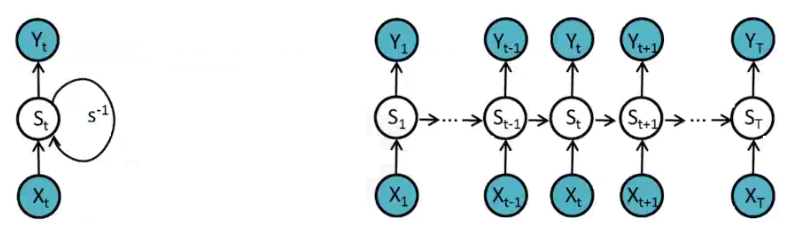
\includegraphics[scale=0.5]{31.png}
\end{center}
Translates an input sequence to an output sequence (\textbf{transduction}). State transition and emission depend on input observations (\textbf{input-driven}).\\
Recursive model highlights analogy with RNNs.
\paragraph{Bidirectional Input-Driven Models} Removes the causality assumption that current observation doesn't depend on the future and homogeneity assumption that a state transition doesn't depend on the position in the sequence.
\begin{center}
	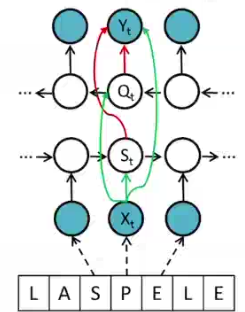
\includegraphics[scale=0.5]{33.png}
\end{center}
\paragraph{Coupled HMMs} Describing interacting processes whose observation follow different dynamics while the underlying generative processes are interlaced.
\begin{center}
	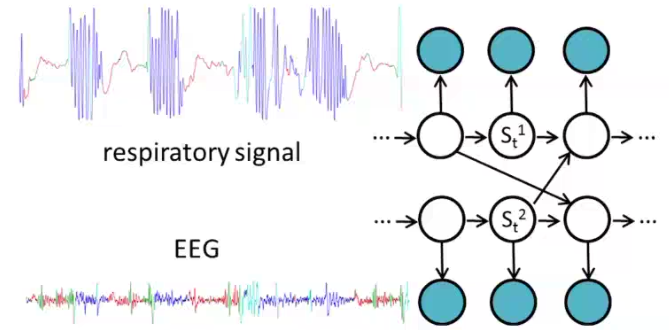
\includegraphics[scale=0.5]{32.png}
\end{center}
\paragraph{Dynamic Bayesian Networks} HMMs are a specific and the simplest case of a class of directed models that represent dynamic processes and data with changing connectivity template. Other examples are: Hierarchical HMMs and structure changing information.\\
DBNs are graphical models whose structure changes to represent evolution across time and/or between different samples.
\subsection{Markov Random Fields}
MFRs are undirected graphs $G = (V, E)$.
\begin{list}{}{}
	\item Nodes $v\in V$ are random variables $X_v$
	\item Edges $e\in E$ are bi-directional dependencies between variables
\end{list}
\paragraph{Likelihood Factorization} Define $X = X_1,\ldots, X_N$ as the random variables associated to the $N$ nodes in the undirected graph $G$
$$P(\text{X}) = \frac{1}{Z}\prod_C \psi_C(X_C)$$\\
$X_C$ are the random variables associated to the maximal clique $C$, $\psi_C(X_C)$ is the \textbf{potential function} for clique $C$\\
With $Z$ normalization term used to transform to probability, from a \textbf{partition function}:
$$Z = \sum_X\prod_C\psi_C(X_C)$$
As already stated, potential functions are not probabilities, they express which configurations of the local variables are preferred. A conveniently and widely used strictly positive representation of the potential function is the \textbf{Boltzmann Distribution}:
$$\psi_C(X_C)=\exp\left(-E(X_C)\right)$$
with $E(X_C)$ called \textbf{energy function}.\\
In general we will assume to work with Markov Random Fields where the partition functions factorize as $$\psi_C(X_C) = \exp\left(-\sum_{k=1}^K\:\underset{\text{Parameters}}{\underbrace{\theta_{Ck}}}\cdot\underset{\text{Feature function}}{\underbrace{f_{Ck}(X_C)}}\right)$$
\begin{list}{}{}
	\item $K$ defines the number of feature functions that we use, so the cardinality of a dictionary of feature functions $f_{Ck}$
	\item $\theta_{Ck}\in\mathbb{R}$ are parameters
\end{list}
Undirected graphical models do not express the factorization of potentials into feature functions, you cannot express $f$ graphically $\Rightarrow$ \textbf{factor graphs}.
\paragraph{Factor Graphs} Random Variables are still circular nodes, factors $f_{Ck}$ are denoted with square nodes and edges connect a factor to the random variable.
\begin{center}
	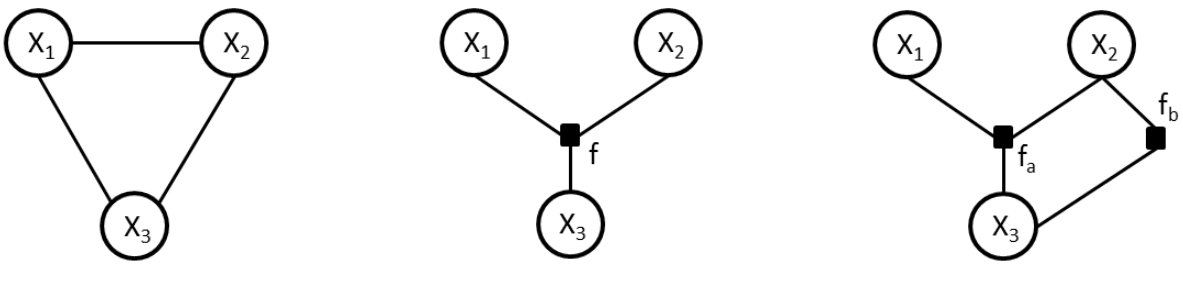
\includegraphics[scale=0.5]{34.png}
\end{center}
$$\psi(X_1,X_2,X_3) = f(X_1,X_2,X_3)$$
$$\psi(X_1,X_2,X_3) = f_a(X_1,X_2,X_3)f_b(X_2,X_3)$$
\paragraph{Sum-Product Inference} A powerful class of \textbf{exact inference algorithms}. Use factor graph representation to provide a unique algorithm for directed/undirected models. So \textbf{factor graph are a "unifying language" to represent both models, directed and undirected}.\\
Inference is \textbf{feasible for chain and tree structures}. We restructure the graph to obtain a tree-like structure to perform message passing (\textbf{junction tree algorithm}) and then do approximated inference (variational, sampling).\\
Even better: we constrain the MRF to obtain tractable classes of undirected models.
\paragraph{Restricting to Conditional Probabilities} In Maximum Likelihood (ML) a part of the random variables can be assumed to be always observable (input data).\begin{list}{}{}
	\item $X_k$ are observable inputs in the factor $k$
	\item $Y_k$ are hidden or partially observable random variables
	\item $f_k(X_k, Y_k)$ is the factor feature function
\end{list}
Instead of $P_\theta(x,y)$ we compute $P_\theta(y\:|\:x)\cdot P_\theta(x)$. Under this assumption we can directly model the conditional distribution $$P(Y\:|\:X) = \frac{1}{Z(X)}\prod_k \exp\left(\theta_kf_k(X_k,Y_k)\right)$$
With the partition function $Z$ now being dependent on $X$, not a general partition function over all the possible values of $X$ but ensures a sum-to-one constraint over a specific $X$
$$Z(X) = \sum_y\prod_k\exp\left(\theta_kf_k(X_k,Y_k = y)\right)$$
\subparagraph{Conditional Random Field} CRF are constrained MRF models representing input-conditional distributions.
\begin{center}
	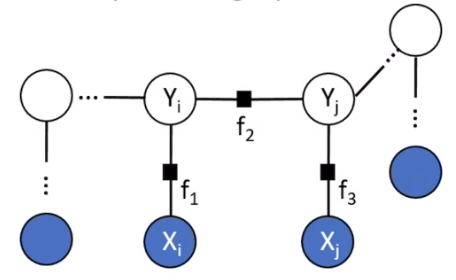
\includegraphics[scale=0.5]{35.png}
\end{center}
$$P(Y\:|\:X,\theta) = \frac{1}{Z(X)}\exp\left(\theta_1f_1(X_i, Y_i) + \theta_2f_2(Y_i,Y_j) + \theta_3f_3(X_j, Y_j)+\ldots\right)$$
\paragraph{Feature Functions} Represent coupling or constraints between random variables, and are often very simple such as linear functions. Examples:
\begin{list}{}{}
	\item Make noisy binary pixel $X_i$ and its clean version $Y_i$ have the same sign: $f_i(X_i,Y_i)=X_iY_i$
	\item Constrain nearby interpretations to be similar: $f_{ij}(Y_i, Y_j) = Y_i^TY_j$
\end{list}

\paragraph{Discriminative Learning in Graphical Models} $X$ is always observable input while $Y$ \textbf{can} be unobserved.\\
Let's consider a single $Y$ and multiple $X$s. Assuming we can observe the $Y_n$ corresponding to $X_n$ for some $n$, we can use this information to fit $\theta$ in $P(Y\:|\:X,\theta)$
\paragraph{CRF for Sequences} Undirected and discriminative equivalent of an HMM.\begin{center}
	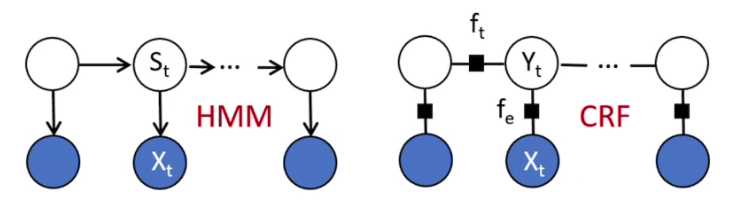
\includegraphics[scale=0.5]{36.png}
\end{center}
\begin{list}{}{}
	\item $f_t(Y_{t-1}, Y_t)$ looks like the transition probability $P(S_t\:|\:S_{t-1})$
	\item $f_e(X_t, Y_t)$ looks like the emission $P(X_t\:|\:S_t)$
\end{list}
But \textbf{I can place as many feature functions $f_t$ I want between the same variables} while I can't place more transition probabilities in the HMM. The other difference is the main essences.
\paragraph{Generalization of HMM} CRF are much more powerful\begin{center}
	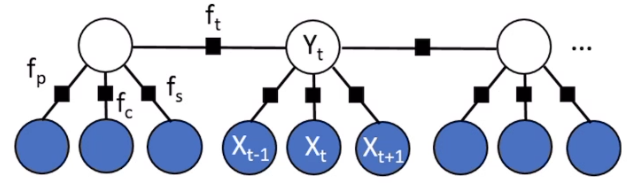
\includegraphics[scale=0.4]{37.png}
\end{center}
Each hidden state may depend on the previous, with $f_t$, but also on the emissions for the previous, current and next symbols. This cannot be easily implemented in HMMs. Kind of time stationality.
$$P(Y\:|\:X,\Theta) = \frac{1}{Z(X)}\prod_t \exp\left(\Theta_pf_p(X_{t-1},Y_t) + \Theta_cf_c(X_t,f_t) + \Theta_sf_s(X_{t+1},Y_t)+\Theta_tf_t(Y_{t-1},Y_t)\right)$$
The cliques to consider are simply $(Y_t, X_{t-1}), (Y_t, X_{t}), (Y_t, X_{t+1}), (Y_t, Y_{t-1})$ for each $t$.\\
We can also model explicitly input influence on transition.
\begin{center}
	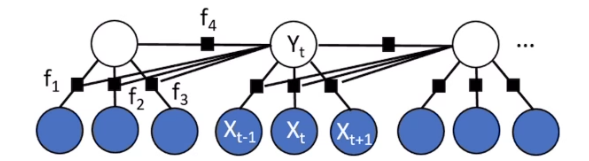
\includegraphics[scale=0.5]{38.png}
\end{center}
The general \textbf{Linear Conditional Random Fields} likelihood is
$$P(Y\:|\:X,\Theta)=\frac{1}{Z(X)}\prod_t\exp\left(\Theta_kf_k(Y_t,Y_{t-1},X_t)\right)$$
Uses indicator variables in $f_k$ definition to include or disregard the influence of specific random variables: e.g. $\mathbf{1}_{Y_t=i}, \mathbf{1}_{X_t=o}$
\paragraph{Posterior Inference in LCRF} The equivalent of the smoothing problem is $P(Y_t, Y_{t-1}\:|\:X)$\\
Solved by exact forward-backward inference. Sum-product message passing (alpha-beta recursion) on the LCRF factor graph.
$$P(Y_t,Y_{t-1}\:|\:X)\simeq\underset{\text{Forward message}}{\underbrace{\alpha_{t-1}(Y_{t-1})}}\underset{\text{Clique weighting}}{\underbrace{\psi_t(Y_t,Y_{t-1},X_t)}}\underset{\text{Backward message}}{\underbrace{\beta_t(Y_t)}}$$
\begin{list}{}{}
	\item \textbf{Clique weighting} $\psi_t(Y_t,Y_{t-1},X_t)=\exp(\Theta_cf_c(X_t,Y_t)+\Theta_tf_t(Y_{t-1},Y_t))$
	\item \textbf{Forward message} $\alpha_t(i) = \sum_j\psi_t(i,j,X_t)\alpha_{t-1}(j)$
	\item \textbf{Backward message} $\beta_t(i) = \sum_i\psi_{t+1}(i,j,X_{t+1})\beta_{t+1}(i)$
\end{list}
Also Viterbi can be used, because we can do Max-Product. The expensive part is the computation of the exponential summation in $Z(X)$. The forward-backward algorithm computes it efficiently as normalization term of $P(Y_t,Y_{t-1}\:|\:X)$. More articulated posteriors interact with $Z(X)$, which is a summation over everything that's not observable, difficult when there's a lot of unobservable variables. Exact inference in CRF other than chain-like is likely to be computationally impractical. We need to approximate: Markov Chain Monte Carlo (sample $y$ rather than estimate $P(y)$) or Variational Belief Propagation (reduce to message passing on trees).
\paragraph{Training LCRF}Maximum (conditional) log-likelihood, for training $$\max_\Theta L(\Theta) = \max_\Theta\sum_{n=1}^N\log P(y^n\:|\:x^n,\Theta)$$
We can substitute the LCRF conditional formulation because $P(y^n\:|\:x^n,\Theta) = \frac{1}{Z(X)}\exp(\sum \Theta_k f_k)$\\
getting $\log \frac{1}{Z(X)}\exp(\sum \Theta_k f_k) = \log \exp(\sum \Theta_k f_k)-\log Z(X)$
$$L(\Theta)=\sum_n\sum_t\sum_k \Theta_kf_k(Y_t^n,Y_{t-1}^n,X_t^n)-\sum_n\log Z(X^n)\underset{\text{Regularization term}}{\underbrace{-\sum_k\frac{\Theta_k^2}{2\sigma^2}}}$$
With the last being a regularization term based on $\|\Theta\|^2$.\\
To get proper marginalization $$Z(X^n) = \sum_{y_t,y_{t-1}}\sum_t \exp\left(\sum_k\Theta_k f_k(y_t,y_{t-1},x^n_t)\right)$$
$$\frac{\partial\log(Z(X))}{\partial \theta_k} = \frac{1}{Z(X)}\cdot\frac{\partial Z(X)}{\partial \theta_k} = \frac{1}{Z(X)}\cdot\sum_{y_t,y_{t-1}}\sum_t\exp\left(\sum_k\theta_k f_k\right)f_k$$
Which looks like
$$P(y^n\:|\:x^n,\Theta) = \frac{1}{Z(X)}\exp\left(\sum_k\theta_kf_k\right)$$
So we have $P(Y\:|\:X) = \frac{1}{Z(X)}\exp\left(\sum_k\theta_k f_k\right)f_k$\\
With $\frac{\partial L(\Theta)}{\partial \Theta_k}$ we can maximize it because typically $L(\Theta)$ cannot be maximized in closed form.
$$\frac{\partial L(\Theta)}{\partial \Theta_k} = \underset{\mathbb{E}_{y,y'\sim\text{ dataset}}[f_k(y,y',X_t^n)]}{\underbrace{\sum_{n,k}f_k(Y_t^n,Y_{t-1}^n,X_t^n)}}-\underset{\mathbb{E}_{P(Y\:|\:X,\theta)}[f_k(y,y',X_t^n)]}{\underbrace{\sum_{n,t}\sum_{y,y'}f_k(y,y',X_t^n)P(y,y'\:|\:X^n_t)}}-\frac{\Theta_k}{\sigma^2}$$ 
We have sum of expectations:
\begin{list}{}{}
	\item the first term is $\mathbb{E}[f_k]$ when $Y$ is not random, with samples drawn from a finite dataset (\textbf{empirical distribution})
	\item the right term is $\mathbb{E}[f_k]$ using the posterior so the expectation of the feature function under the \textbf{model distribution}
\end{list}
$$\frac{\partial L(\Theta)}{\partial \Theta_k} = \mathbb{E}_{y,y'\sim\text{ dataset}}[f_k(y,y',x^n_t)] - \mathbb{E}_{P(Y\:|\:X,\Theta)}[f_k(y,y',x_t^n)]$$
We need to match those two expectations, meaning that when the gradient is zero these are equal. So \textbf{Maximum Likelihood learning makes sure that the model expectation matches the empirical expectation}: it's a general property of exponential models.\\
There's a regularization term $\sum_k\frac{\Theta_k^2}{2\sigma^2}$ on $\|\Theta\|^2$, a posteriori regularization on the gaussian $P(\Theta)$ with $\mu=0$ mean and $\sigma^2I$ variance.\\
In practice, then, $\Theta$ can be learn with stochastic gradient descent or variants.
$$\theta^m = \theta^{m-1} - v_m\nabla L_n(\theta^{m-1})$$
$$\nabla L_{nk}(\theta) = \sum_t f_k(Y_t^n,Y_{t-1}^n,X_t^n)-\sum_t\sum_{y,y'}f_k(y,y',X_t^n)P(y,y'\:|\:X^n)-\frac{\theta_k}{N\sigma^2}$$
(remembering to divide the regularization by the number of terms $N$), with$P(y,y'\:|\:X^n)$ estimated by sum-product inference.
\paragraph{Applications} Linear CRF have various applications: POS-tagging, semantic role identification, bioinformatics. Feature functions have the form $f_k(X_k,Y_k)=I_{y_k=\hat{y}_k}q(X_c)$, with $f_k$ non-zero only for a specific output configuration $\hat{y}_k$, and then depending only on $X_k$ (the features not shared by the classes). $q(X_c)$ is the observation functions: word begins with capital, ends with -ing\ldots\\
In computer vision they can be used to define bi-dimensional lattice on images, bg/fg segmentation and to impost constraints.
\subsection{Bayesian Learning and Variational Inference}
Introducing basic concepts of variational learning useful for both generative models and deep learning.
\begin{list}{}{}
	\item \textbf{Bayesian Latent Variable} models: class of generative models for which variational or approximated methods are needed
	\item \textbf{Latent Dirichlet Allocation}: possibly the simplest Bayesian latent variable model, with many applications in unsupervised text analytics, machine vision,\ldots
\end{list}
\paragraph{Latent Variables} \textbf{Unobserved random variables that define a hidden generative process of observed data}. They explain the complex relations between many observable variables. Examples of latent variables are the hidden states in HMM/CRF.\\
Latent variables likelihood $$P(x) = \int_\mathbf{z}\:\:\prod_{i=1}^N  P(x_i\:|\:z)\cdot P(\mathbf{z})\:\:d\mathbf{z}$$ with a graph like $Z \longrightarrow X$ so of nodes $\{Z,X\}$ and a directed arc $(Z,X)$.
\paragraph{Latent Spaces} Spaces where high-dimensional data can be represented. Each of the $M$ samples is made of $N$ features represented internally with $k<<N$ dimensions.
\begin{center}
	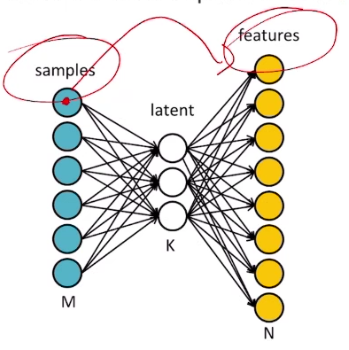
\includegraphics[scale=0.5]{39.png}
\end{center}
The assumption is that latent variables conditional and marginal distribution are more tractable than the joint distribution $P(X)$.
\paragraph{Tractability} Introducing hidden variables can make the posteriors intractable. We need stuff that simplify those posteriors: Bayesian learning introduces priors which introduce integrals in the posteriors computation which are not always analytically or computationally tractable.
\subsubsection{Kullback-Leibler Divergence}
An information theoretic measure of closeness of two distributions $p$ and $q$ $$KL(q\|p) = \mathbb{E}_q\left[\log\frac{q(z)}{p(z\:|\:x)}\right] = \mathbb{E}_q[\log q(z)] - \mathbb{E}_q[\log p(z\:|\:x)]$$
Tells how the distribution $q$ differs from $p$. It's a divergence so it is asymmetric, $KL(q\|p) \neq KL(p\|q)$\begin{list}{}{}
	\item if $q$ and $p$ are high, then $KL(q\|p)\simeq 0$
	\item if $q$ is high and $p$ is low, then there's divergence so $KL(q\|p)$ it's large
	\item if $q$ is low we don't care, due to the expectation
\end{list}
The expectation $\mathbb{E}_q$ means taking all possible assignments $z$ weighted according to the probability $q(z)$
$$\mathbb{E}_Q[P(Z)] = \sum_z P(Z)\cdot Q(Z)$$
\paragraph{Jensen Inequality} Property of linear operators on convex/concave functions $$\lambda f(x) + (1-\lambda)f(x)\geq f(\lambda x + (1-\lambda)x)$$
Which generalizes to
$$\frac{\sum_ia_if(x_i)}{\sum_ia_i}\geq f\left(\frac{\sum_ia_ix_i}{\sum_ia_i}\right)$$
The curve is longer than the line connecting the two points. With concave we have $\leq$. Applied to probability $$f(\mathbb{E}[X])\geq \mathbb{E}[f(X)]$$
$$\log(\mathbb{E}[X])\geq \mathbb{E}[\log(X)]$$
The log-likelihood for a model with a single hidden variable $Z$ and parameters $\theta$ with a single sample assumed for simplicity is the following
$$\log P(x\:|\:\Theta) = \log\int_zP(x,z\:|\:\Theta)dz = \log\int_z\frac{Q(z\:|\:\phi)}{Q(z\:|\:\phi)}P(x,z\:|\:\Theta)dz$$
$Q$ is a distribution, used over $z$ with parameters $\phi$ and $Q(z\:|\:\phi)\neq 0$. That is the definition of expectation, we have $\int_zQ(z\:|\:\phi)\cdot \frac{1}{Q(z\:|\:\phi)}P(x,z\:|\:\Theta)$ which is $\sum_z q\cdot g(z)$. Using Jensen we have $$\log P(x\:|\:\Theta)= \log \mathbb{E}_Q\left[\frac{P(x,z)}{Q(z)}\right] \geq \mathbb{E}_Q\left[\log \frac{P(x,z)}{Q(z)}\right]= \underset{\text{Expectation of joint distribution}}{\underbrace{\mathbb{E}_Q[\log P(x,z)]}} - \underset{\text{Entropy}}{\underbrace{\mathbb{E}_Q[\log Q(z)]}} = L(x,\Theta,\phi)$$
So we are lower bounding $\log P(x\:|\:\Theta)$ with the expected joint distribution minus the entropy. So we have a lower bound on something I want to maximize: we can maximize the lower bound. Maximizing this term entails that we're supported by the data (using the expectation of joint distribution $E_Q[\log P(x,z)]$).\\
How good is this lower bound? Meaning $\log P(x\:|\:\Theta) - L(x,\Theta,\phi) = ?$ We introduce $Q(z)$ by marginalization $$\int_z Q(z)\log P(x) - \int_z Q(z)\log\frac{P(x,z)}{Q(z)} = \int_z Q(z)\log\frac{P(x)Q(z)}{P(x,z)}=\mathbb{E}_Q\left[\log \frac{Q(z)}{P(z\:|\:x)}\right] = KL\left(Q(z\:|\:\phi)\|P(z\:|\:x,\Theta)\right)$$
Because $\frac{P(x)}{P(x,z)} = \frac{1}{P(z\:|\:x)}$. So it's an optimization problem of finding $\Theta$ and $\phi$ that maximize $L(x,\Theta,\phi)$ reduced to a minimization problem with KL.\\
We can assume the existence of a probability $Q(z\:|\:\phi)$ which allows to bound the likelihood $P(x\:|\:\Theta)$ from below using $L(x,\Theta,\phi)$.\\
$L(x,\Theta,\phi)$ is called \textbf{variational bound} or \textbf{ELBO} (evidence lower bound). The optimal bound is obtained from $KL\left(Q(z\:|\:\phi)\|P(z\:|\:x,\Theta)\right) = 0$ choosing $Q(z\:|\:\phi)=P(z\:|\:x,\Theta)$. So the problem now becomes maximizing ELBO. Maximum Likelihood learning with hidden variables can be approached by maximization of the ELBO $$\max_{\Theta,\phi}\sum_{n=1}^N L(x_n,\Theta,\phi)$$ where $\Theta$ are the model parameters and $\phi$ is used in $Q(z\:|\:\phi)$.
If $P(z\:|\:x,\Theta)$ is tractable then we use it as $Q(z\:|\:\phi)$ (optimal ELBO). Otherwise we choose $Q(z\:|\:\phi)$ as a tractable family of distributions: find $\phi$ that minimize $KL(Q(z\:|\:\phi)\|P(z\:|\:x,\Theta))$ or find $\phi$ that maximize $L(\:,\phi)$.
\paragraph{Example} Bag of Words representations are classical examples of multinomial data. A BOW dataset $X$ is the $N\times M$ document matrix, with $N$ number of vocabulary items $w_j$ and $M$ is the number of documents $d_i$ and $x_{ij} = n(w_j,d_i)$ the number of occurrences of $w_j$ in $d_i$.\\
Often $M$ is very very large ($\simeq 30$k elements). So we want a smaller representation. Mixture of topics: a topic identifies a pattern in the co-occurrence of multinomial items $w_j$ within the documents. Mixture, so we associate an interpretation (topic) to each item in a document, whose interpretation is then a mixture of the items' topics. We use Latent Variables.
\paragraph{Latent Dirichlet Allocation} LDA models a document as a mixture of topics $z$. We assign one topic $z$ to each item $w$ with probability $P(w\:|\:z,\beta)$ and pick a topic for the whole document with probability $P(z\:|\:\Theta)$
\begin{multicols}{2}
\begin{list}{}{}
	\item $P(w\:|\:z,\beta)$ \textbf{multinomial} item-topic distribution
	\item $P(z\:|\:\theta)$ \textbf{multinomial} topic distribution with document-specific parameter $\theta$
	\item $P(\theta\:|\:\alpha)$ \textbf{Dirichlet} distribution with hyperparameter $\alpha$\\
	It's a distribution for vectors that sums to 1 (\textbf{simplex}): the elements of a multinomial are vector that sums to 1.
\end{list}
\begin{center}
	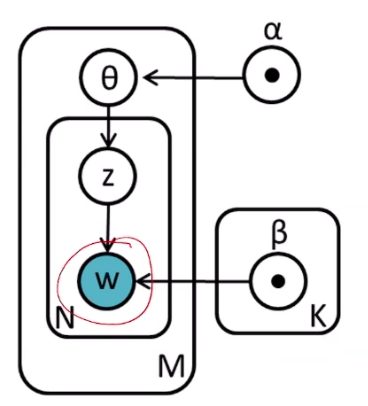
\includegraphics[scale=0.45]{40.png}
\end{center}
\end{multicols}
Each document has its personal topic proportion $\Theta$ sampled from a distribution. $\Theta$ defines a multinomial distribution, but it is a random variable as well. $\alpha$ is the prior.
\paragraph{Dirichlet distribution} Conjugate prior to multinomial distribution.\\
If the likelihood is multinomial with a Dirichlet prior, then posterior is Dirichlet.
$$P(\Theta\:|\:\alpha) = \frac{\displaystyle \Gamma\left(\sum_{k=1}^K \alpha_k\right)}{\displaystyle \prod_{k=1}^K\Gamma(\alpha_k)}\prod_{k=1}^K\Theta_k^{\alpha_k-1}$$
$\Gamma$ is the generalization of the factorial, $\alpha_k$ is the Dirichlet parameter and is a prior count of the $k$th topic which controls the mean shape and sparsity of multinomial parameters $\theta$.
\begin{list}{}{}
	\item $\alpha$ larger means that the topics are almost equiprobable, so every document can express each topic
	\item $\alpha$ lower provides substantially different proportions, almost deterministic
\end{list}
Usually $\alpha \simeq 1$ or smaller.\\\\
LDA finds a set of $K$ projection functions on the $K$-dimensional topic simplex.\begin{center}
	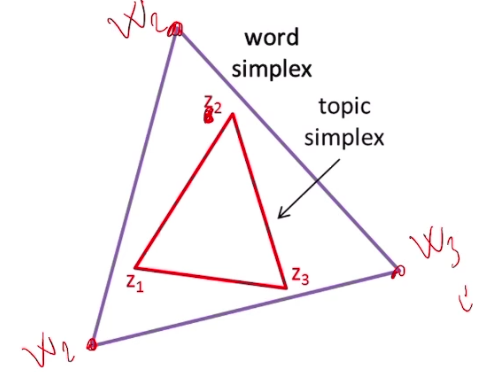
\includegraphics[scale=0.5]{41.png}
\end{center}
\paragraph{LDA Generative Process} For each of the $M$ documents, we choose $\Theta$ with Dirichlet($\alpha$) and for each of the $N$ items, we choose a topic $z$ with Multinomial($\Theta$) and pick an item $w_j$ with multinomial probability $P(w_j\:|\:z,\beta)$.\\
We get a multinomial topic-item parameter matrix $[\beta]_{k\times V}$
$$\beta_{kj}=P(w_j=1\:|\:z_k=1)\text{ or } P(w_j=1\:|\:z=k)$$
$$P(\Theta, z, w\:|\:\alpha,\beta) = P(\Theta\:|\:\alpha)\prod_{j=1}^NP(z_j\:|\:\Theta)P(w_j\:|\:z_j,\beta)$$
It's a completed likelihood with the conditional independence assumption.
\subparagraph{Learning} Marginal distribution of a document $d =$ w
$$P(\text{w}\:|\:\alpha,\beta) = \int \sum_z P(\Theta,z,w\:|\:\alpha,\beta)d\Theta=\int P(\Theta\:|\:\alpha)\prod_{j=1}^N\sum_{z_j=1}^kP(z_j\:|\:\Theta)P(w_j\:|\:z_j,\beta)d\Theta$$
given w$_1$,\ldots,w$_M$ find $\alpha,\beta$ that maximize.\\
Key problem is inferring latent variables posterior, because optimal ELBO is achieved when $Q(z)$ is equal to the latent variable posterior:
$$P(\Theta, \text{z}\:|\:\text{w},\alpha,\beta) = \frac{P(\Theta, \text{z}, \text{w}\:|\:\alpha,\beta)}{P(\text{w}\:|\:\alpha,\beta)}$$
but the denominator is intractable because of couplings between $\beta$ and $\Theta$ under exponenziation in the summation over topics. So we don't use the posterior, we pick a function $Q$ that helps in solving the problem (variational inference).
\paragraph{Variational Inference} We write $Q(z\:|\:\phi)$ function that is sufficiently similar to the posterior but tractable. It should be such that $\beta$ and $\Theta$ are no longer coupled, fitting $\phi$ so that is close to the posterior according to KL.\\
Fast convergence but it's an approximation.\\
The key idea is to assume that $Q(z\:|\:\phi)$ is factorizable (\textbf{tractable}): \textbf{mean-field assumption}.
$$Q(z\:|\:\phi) = Q(z_1,\ldots,z_K\:|\:\phi)=\prod_{k=1}^K Q(z_k\:|\:\phi_k)$$
Can be generalized by factorizing on groups of latent variables. Does not contain the true posterior because hidden variables are dependent.\\
We optimize ELBO using $Q(z\:|\:\phi)$ factorized distribution. Simple \textbf{coordinate ascent inference}: iteratively optimize each variational distribution holding the others fixed, so when learning we use the model on the right, breakdown of the independence.
\begin{center}
	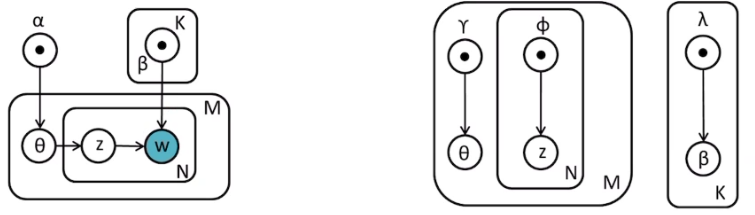
\includegraphics[scale=0.5]{42.png}
\end{center}
Given $\Phi=\{\gamma,\phi,\lambda\}$ as \textbf{variational approximation parameters}.
$$Q(\theta,z,\beta\:|\:\Phi) = Q(\theta\:|\:\gamma)\prod_{n=1}^NQ(z_n\:|\:\phi_n)\prod_{k=1}^KQ(\beta_k\:|\:\lambda_k)$$
Then we have the model parameters $\Psi=\alpha,\beta$ of sample distribution $P(\theta,z,w\:|\:\alpha,\beta)=P(\theta,z,w\:|\:\Psi)$
\paragraph{Variational Expectation-Maximization} Find the $\Phi, \Psi$ that maximize the ELBO
$$L(w,\Phi,\Psi) = \mathbb{E}_Q[\log P(\Theta,z,w\:|\:\Psi)] - \mathbb{E}_Q[\log Q(\Theta,z,\Psi\:|\:\Phi)]$$
by alternate maximization:
\begin{list}{}{}
	\item Fix $\Psi$ and update variational parameters $\Psi^*$ (\textbf{E-Step})
	\item Fix $\Phi = \Phi^*$ and update the model parameters $\Psi^*$ (\textbf{M-Step})
	\item Repeat until little improvement on the likelihood
\end{list}
Unlike EM, variational EM has no guarantee to reach a local maximizer of $L$.
\pagebreak
\subsection{Boltzmann Machines}
Examples of Markov Random Fields:
\begin{multicols}{2}
\begin{list}{}{}
	\item Visible random variables $v\in\{0,1\}$
	\item Latent random variables $h\in\{0,1\}$
	\item $s = [vh]$ (concatenation)
\end{list}
\columnbreak
\begin{center}
	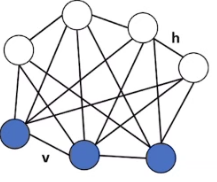
\includegraphics[scale=0.5]{46.png}
\end{center}
\end{multicols}
Linear energy function $$E(s) = -\frac{1}{2}\sum_{ij}M_{ij}s_is_j - \sum_jb_js_j = -\frac{1}{2}s^TMs - b^Ts$$
with symmetric and no self-recurrent connectivity. Model parameters $\Theta = \{M, b\}$ encode the interactions between the variables (observable and not).\\
\textbf{Boltzmann machines are a type of Recurrent Neural Networks}. They can be interpreted as stochastic neural network: the state of a unit at a given timestep is sampled from a given probability distribution and the network learns a probability distribution $P(V)$ from the training patterns. The network includes both visible $v$ and hidden $h$ units, and the activity is a sample from posterior probability given the inputs (visible data).
\paragraph{Stochastic Binary Neurons} Binary output $s_j$ at any time $t$. Typically discrete time model with time into small $\Delta t$ intervals. At each time interval $t+1 = t+\Delta t$ the neuron can emit a spike with probability $p_j^{(t)}$ $$s_j^{(t)} = \left\{\begin{array}{c l}
1&\text{with probability }p_j^{(t)}\\
0&\text{with probability }1-p_j^{(t)}
\end{array}\right.$$
The key is in the definition of the spiking probability (needs to be a function of \textbf{local potential} $x_j$) $$p_j^{(t)} \simeq \sigma(x_j^{(t)})$$
The Boltzmann machine has $N$ neurons with binary activations $s_j$, a weight matrix $M = [M_{ij}]_{i,j} \in \{1,\ldots,N\}$ and a bias vector $b = [b_j]_j\in\{1,\ldots,N\}$\\
Local neuron potential $x_j$ is the usual $$x_j^{(t+1)} = \sum_{i=1}^N M_{ij}s_j^{(t)} +b_j$$
This assuming full connectivity with weight $0$ if you want to ignore a neuron in the potential. A chosen neuron fire with spiking probability which is a sigmoid $$p_j^{(t+1)} = P\left(s_j^{(t+1)} = 1\:|\:s^{(t)}\right) = \sigma\left(x_j^{(t+1)}\right) = \frac{1}{1+e^{-x_j^{(t+1)}}}$$
Clearly has Markovian dynamics, $P(s^{(t+1)}\:|\:s^{(t)})$\\\\
How does the model state (activation of all neurons) evolve in time?
\paragraph{Parallel Dynamics} Assuming we can compute each activation in parallel every $\Delta t$, updating each random variable in parallel. $$P\left(s^{(t+1)}\:|\:s^{(t)}\right) = \prod_{j=1}^N P\left(s_j^{(t+1)}\:|\:s^{(t)}\right) = T\left(s_j^{(t+1)}\:|\:s^{(t)}\right)$$
Yielding a Markov process for state update
$$P\left(s^{(t+1)} = s'\right) = \sum_s T\left(s'\:|\:s\right)P\left(s^{(t)} = s\right)$$
\paragraph{Glauber Dynamics} One neuron at random is chosen for update at each step. No fixed-point guarantees for $s$, but it has a stationary distribution for the network at equilibrium state when its connectivity is symmetric.\\
Given $F_j$ as a state flip operator for the $j$the random variable $s^{(t+1)}=F_js^{(t)}$
$$T(s^{(t+1)}\:|\:s^{(t)}) = \frac{1}{N}P(s_j^{(t+1)}\:|\:s^{(t)})$$
\subparagraph{Boltzmann-Gibbs Distribution} Undirected connectivity enforces detailed balance condition $$P(s)T(s'\:|\:s) = P(s')T(s\:|\:s')$$
Ensures reversible transitions guaranteeing existence of equilibrium distribution (Boltzmann-Gibbs) $$P_\infty(s) = \frac{e^{-E(s)}}{Z}$$
where $E(s)$ is the energy function and $Z = \sum_se^{-E(s)}$ is the partition function.
\paragraph{Learning} Boltzmann machines can be trained so that the equilibrium distribution tends towards any arbitrary distribution across binary vectors given samples from that distribution. Basically, you can represent any distribution of binary variables.\\
Couple of simplifications:
\begin{list}{}{}
	\item bias $b$ is just another row in the weight matrix $M$
	\item consider only visible random variables, meaning $s = v$
\end{list}
We use probabilistic learning techniques to fit the parameters, i.e. maximizing the log-likelihood (note that $\langle x\rangle = \mathbb{E}[x]$) $$L(M)=\frac{1}{L}\sum_{l=1}^L \log P(v_l\:|\:M)$$
given the $L$ visible training patterns $v_l$, the set of all the visible units (so it's a joint distribution $v_{l1},\ldots,v_{ln}$). We need a way to write the likelihood $P(v_l\:|\:M)$, and we can use the Boltzmann-Gibbs. So we can optimize it solving a maximum likelihood problem.
$$\log P(v_l\:|\:M) = \log \frac{e^{-E(v)}}{Z} = -E(v) - \log Z$$
$$\frac{\partial L}{\partial M_{ij}} = \frac{\partial (-E(v) - \log Z)}{\partial M_{ij}}\Leftrightarrow$$
Given that $E(v) = -\frac{1}{2}v^TM^Tv = -\sum_{ij} M_{ij} v_iv_j$ we get that every $M_{ij}$ will be constant except for the $M_{ij}$ we are differentiating leaving with $v_iv_j$. As for $\log Z$, differentiating the potential function leaves us with $\sum_v P(v\:|\:M)v_iv_j$ from $\partial\log\partial\exp\cdot\partial E$
$$\Leftrightarrow v_iv_j - \sum_v P(v\:|\:M)v_iv_j = 0$$
The second term is $\sum_v P(v\:|\:M)v_iv_j = \mathbb{E}_{v_iv_j\in P(v\:|\:M)}[v_iv_j] = \langle v_iv_j\rangle_M$ the expectation of the coactivation of two units $v_i,v_j$ when the values of those two units are taken from $P(v\:|\:M)$ the distribution learned by the model $M$.\\
So for a single $l$:
$$v_i^lv_j^l - \langle v_iv_j\rangle_M$$
not introducing $l$ in the second term because it's marginalized, all the possible values in all possible configurations, it's an expectation and the data is already included in the formulation.\\
So $\forall\:v^l\in L$ $$\frac{\partial L}{\partial M_{ij}} = \frac{1}{L}\sum_{l=1}^L (v_i^lv_j^l)-\langle v_iv_j\rangle_M=$$
We have the clamped expectation under the empirical distribution $\frac{1}{L}\sum_{l=1}^L (v_i^lv_j^l) = \mathbb{E}_{v_i^lv_j^l\in L}[v_i^lv_j^l] = \langle v_iv_j\rangle_c$
$$=\underset{\text{Wake}}{\underbrace{\langle v_iv_j\rangle_c}} - \underset{\text{Dream}}{\underbrace{\langle v_iv_j\rangle_M}} = \Delta M_{ij}$$
So we're focusing on the neurons $i, j$ and the link between them $M_{ij}$, and we increase the connection when both are 1 so when $\langle v_iv_j\rangle_c$ is larger, so Hebbian learning. The second term $\langle v_iv_j\rangle_M$, if they are in disagreement then they are flipped then it's zero, if instead they are coactive (both on or off) then it's close to $-1$. It's anti-Hebbian, has the purpose of nearing the expectation of the model towards the reality.\\
When $\langle v_iv_j\rangle_c - \langle v_iv_j\rangle_M = 0-1$, we have that the model thinks that they are correlated while in reality they are different, so the model stops believing that they are correlated.\\\\
With hidden variables doesn't change much. We have $s=[hv]$
The wake hebbian term $\sum_h s_is_jP(h\:|\:v)$ and the dream anti-hebbian term $\sum_ss_is_jP(s)$
$$\frac{\partial P(v\:|\:M)}{\partial M_{ij}} = \sum_h s_is_jP(h\:|\:v) - \sum_ss_is_jP(s) = \langle s_is_j\rangle_c - \langle s_is_j\rangle_M = \Delta M_{ij}$$
Again intractable. So we restrict.
\paragraph{Restricted Boltzmann Machines} RBM are special Boltzman machines: bipartite graphs and connections only between hidden and visible units, not with "themselves".
\begin{center}
	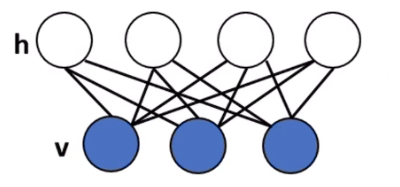
\includegraphics[scale=0.5]{47.png}
\end{center}
This becomes tractable because we can compute the activation of each hidden in parallel and then compute the visible. The energy function is a specialization that higlights the bipartition in hidden and visible units $$E(v,h) = -v^TMh - b^Tv - c^Th$$
Hidden units are conditionally independent given visible units and viceverse
$$P(h_j\:|\:v)=\sigma\left(\sum_i M_{ij}v_i+c_j\right)$$
$$P(v_i\:|\:h)=\sigma\left(\sum_j M_{ij}h_j+b_i\right)$$
Training is again based on the likelihood maximization $$\frac{\partial L}{\partial M_{ij}} = \underset{\text{Data}}{\underbrace{\langle v_ih_j\rangle_c}} - \underset{\text{Model}}{\underbrace{\langle v_ih_j\rangle}} = \Delta M_{ij}$$
Again, we have data $-$ model which are both expectations that need to be estimated. The first has the sum on just $h$, the second is a full summation over both $v$ and $h$.\\
With a Gibbs sampling approach:
\begin{multicols}{2}
For the wake/data term\begin{list}{}{}
	\item Clamp data on $v$
	\item Sample $v_ih_j$ for all pairs of connected units
	\item Repeat for all elements of the dataset as to stay as near as possible to the empirical data
\end{list}
\columnbreak

For the dream/model term\begin{list}{}{}
	\item Don't clamp units
	\item Let network reach equilibrium
	\item Sample $v_ih_j$ for all pairs of connected units
	\item Repeat many times to get a good estimate
\end{list}
\end{multicols}
Computing a correlation between ideally $v^\infty,h^\infty$, but of course can't wait until the infinity sample and we cut at some sample $k$ so $v^k,h^k$.
\begin{center}
	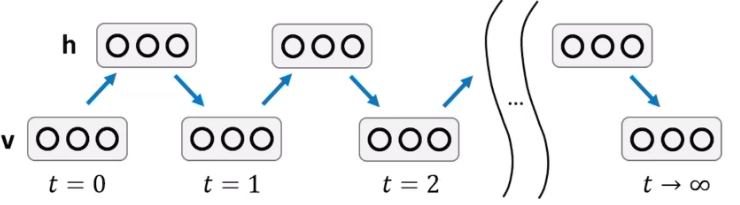
\includegraphics[scale=0.5]{48.png}
\end{center}
We start with a training vector on the visible units, alternating between updating all the hidden units in parallel and updating all the visibile units in parallel
$$\frac{\partial L}{\partial M_{ij}} = \underset{\text{data}}{\underbrace{\langle v_ih_i\rangle_0}} - \underset{\text{model}}{\underbrace{\langle v_jh_j\rangle_\infty}}$$
\paragraph{Contrastive-Divergence Learning} Because Gibbs sampling converges really slowly: clamp a training vector $v^l$ on visible units. CD-1.
\begin{center}
	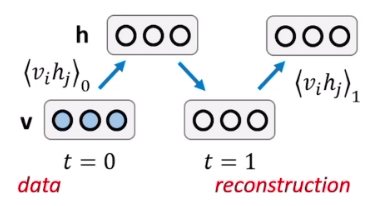
\includegraphics[scale=0.5]{49.png}
\end{center}
Clamping a training vector $v^l$ on visible units, update all hidden units in parallel, update all the visible units in parallel to get a \textbf{reconstruction} and update the hidden units again.
$$\underset{\text{data}}{\underbrace{\langle v_ih_j\rangle_0}}-\underset{\text{reconstruction}}{\underbrace{\langle v_ih_j\rangle_1}}$$
Learns a very crude approximation of the gradient of log-likelihood, not even following it closely. Why use it? Because in practice it works well.
\subsection{Wrap Up}
We've seen three families of models\begin{list}{}{}
	\item \textbf{Bayesian Networks}: unsupervised data understanding, interpretability but weak on supervised performance. Directed.
	\item \textbf{Markov Random Fields}: undirected version of BN, powerful when knowledge and constraints can be expressed with dictionaries. CRF: supervised way to be generative.\\
	But computationally heavy.
	\item \textbf{Dynamic Models}: topology unfolds on data structure, structured data processing but complex causal relationships.
\end{list}
\paragraph{Tractability} Generative models to be used when:
\begin{list}{}{}
	\item Need interpretability
	\item Need to incorporate prior knowledge
	\item Unsupervised learning or learning with partially observable supervision
	\item Need reusable/portable knowledge
\end{list}
To be avoided when:
\begin{list}{}{}
	\item Having tight computational constraints
	\item Dealing with raw, noisy, low-level data
\end{list}
Variational inference and sampling are efficient ways to learn approximations to intractable distribution. Neural networks can be used as variational functions or to implement sampling processes.
\section{Sampling Methods} 
\paragraph{Sampling} Drawing a set of realizations $X = \{x_1,\ldots,x_L\}$ of a random variable $x$ with a distribution $p(x)$. The set contains $L$ samples.\\
If we have a sampling set we can use it to approximate $p(x)$ using the \textbf{empirical distribution} $$p(x)\simeq \frac{1}{L}\sum_{l=1}^L I[X_l = x]$$ with $I[c] = 1 \Leftrightarrow c$ is true.\\
We can also approximate the expectation of a function $f$ $$\mathbb{E}_{p(x)}[f(x)]\simeq \frac{1}{L}\sum_{l=1}^L f(x_l)$$
We need sampling when $p(x)$ is intractable. For example, in Bayesian models the parameters are random variables but the posteriors are often intractable so we can use sampling to obtain the model parameters.
\paragraph{Sampling Procedure as Distributions} A sampler $S$ is a procedure that generates a sample set $X$ from a generic distribution $p(x)$. Since $X$ contains realizations of random variables, also $X$ has a probability distribution. We denote with $\hat{p}_S(X)$ the probability to obtain the sample set $X$ from the sampler $S$.\\
A \textbf{sampler} and its properties \textbf{are fully defined by its distribution} $\hat{p}_S(X)$. In general
$$\hat{p}(X) \neq p(x)$$
\begin{list}{}{}
	\item $p(x)$ is the distribution we would like to sample from, usually intractable
	\item $\hat{p}(X)$ is the distribution over the samples set and defined by the sampling procedure
\end{list}
Let us consider the sampling approximation of the expectation
$$\mathbb{E}_{p(x)}[f(x)]\simeq \frac{1}{L}\sum_{l=1}^L f(x_l) = \hat{f}_X$$
Since $\hat{f}_X$ estimates a value, we could ask:
\begin{list}{}{}
	\item Is $\hat{f}_X$ an unbiased estimator?
	\item How much is the variance of the approximation?
\end{list}
An unbiased estimator $\hat{\Theta}$ of the unknown $\Theta \Rightarrow$ the approximation is exact on average. Meaning: let $\hat{p}(X)$ the distribution over all possible realizations of the sampling set $X$, then $\hat{f}_X$ is unbiased estimator if $$\mathbb{E}_{\hat{p}(X)}[\hat{f}_X] = \mathbb{E}_{p(x)}[f(x)]$$
This is true provided that $\hat{p}(x_l) = p(x_l)$\\
A sampler with this property is called \textbf{valid} because it draws samples from the desired distribution.\\\\
The variance of $\hat{f}(X)$ tells us how much we can rely on the approximation computed using the sampling set $X$. Let $$\Delta\hat{f}_X = \hat{f}_X - \mathbb{E}_{\hat{p}(X)}[\hat{f}_X]$$ then the variance of $\hat{f}(X)$ is given by $\mathbb{E}_{\hat{p}_X}[(\Delta\hat{f}_X)^2]$ and we would like low variance meaning that $\hat{f}(X)$ is quite always close to the average, i.e. to $\mathbb{E}_{p(X)}[f(X)]$.\\\\
So if the sampler has same marginals $(\hat{p}(x_l)=p(x_l))$ and draws sample independently $(\hat{p}(x_l,x_{l'}) = \hat{p}(x_l)\hat{p}(x_{l'}))$ we obtain $$\mathbb{E}_{\hat{p}_X}[(\Delta \hat{f}_X)^2] = \frac{1}{L}\text{Var}_{p(x)}[f(x)]$$
The variance reduces linearly with respect to the number of samples provided that $\text{Var}_{p(x)}[f(x)]$ is finite.\\\\
We've shown that we need sampling to approximate expectations and to do inference in Bayesian models. Properties of the sampling procedure depends on $\hat{p}(X)$:
\begin{list}{}{}
	\item \textbf{Valid Sampler}: $\hat{p}(x_l) = p(x_l)$
	\item \textbf{Low Approximation Variance}: $\hat{p}(x_l,x_{l'}) = \hat{p}(x_l)\hat{p}(x_{l'})$
\end{list}
\pagebreak
\subsection{Univariate Sampling}
Easy: random number generator $R$ which produces a value uniformly at random in $[0,1]$ and $p(x)$. We use $p(x)$ to divide $[0,1]$ in bins and sample accordingly.
\subsection{Multivariate Sampling}
In the multivariate case $p(x)$ represents a joint distribution over a set of discrete variables $\{s_1,\ldots,s_n\}$ each with $C$ states. Hence each sample $x_i\in X$ contains $n$ values.\\
We build a univariate distribution $p(S)$ where $S$ is a discrete variables with $C^n$ states (all possible combinations) and we can sample from $p(S)$ using the univariate schema.
\begin{center}
	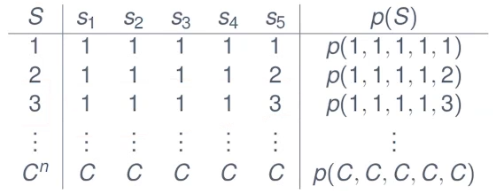
\includegraphics[scale=0.5]{44.png}
\end{center}
The problem is the number of possible states $C^n$, so computationally unfeasible.\\
Using the chain rule we can rewrite the joint distribution as a chain of conditional distributions. Then we sample in order:
\begin{list}{}{}
	\item $\hat{s}_1 \simeq p(s_1)$
	\item $\hat{s}_2 \simeq p(s_2\:|\:\hat{s}_1)$
	\item \ldots
	\item $\hat{s}_n \simeq p(s_n\:|\:\hat{s}_1,\ldots,\hat{s}_{n-1})$
\end{list}
Each is univariate, so easy, but unfortunately computing the distribution $p(s_i\:|\:s_{j<i})$ often requires summation over an exponential number of states.\\
This approach is called \textbf{Ancestral Sampling}, and it's a valid sampler since each sample $x_l$ is drawn from $p(x)$. It also has low variance since the samples are independent. There are cases where it cannot be used.
\subparagraph{Example} We can apply directly if a distribution $p(s_1,\ldots,s_n)$ is already presented as a belief network:
\begin{center}
	\includegraphics[scale=0.5]{67.png}
\end{center}
The BN ancestral order tells us the sampling order
$$\{s_1,s_2,s_4\}\prec\{s_3\}\prec\{s_6\}\prec\{s_5\}$$\begin{list}{}{}
	\item Sample $\hat{s}_1\simeq p(s_1)$
	\item Sample $\hat{s}_4\simeq p(s_4)$
	\item Sample $\hat{s}_2\simeq p(s_2)$
	\item Sample $\hat{s}_3\simeq p(s_3)$
	\item Sample $\hat{s}_6\simeq p(s_6)$
	\item Sample $\hat{s}_5\simeq p(s_5)$
\end{list}
We obtain a single sample $x^l = \hat{s}_1,\hat{s}_2,\hat{s}_3,\hat{s}_4,\hat{s}_5,\hat{s}_6$.\\\\
Suppose a subset $s_\epsilon$ of variables that are visible, with $s=s_\epsilon\cup s_{\setminus\epsilon}$ we want to sample from $$P(s_{\setminus\epsilon}\:|\:s_\epsilon) = \frac{p(s_{\setminus\epsilon}, s_\epsilon)}{p(s_\epsilon)}$$
Can we still use Ancestral Sampling?\begin{list}{}{}
	\item Clamping variables changes the structure of the Bayesian network, and computing the new structure is as complex as running exact inference.
	\item We could run AS on the original structure and discarding any samples which do not match the evidence, but we could discard a lot of samples.
\end{list}
Sampling under evidence is very important, in probabilistic models the inference is based on the posterior which is exactly that. With set $h$ of hidden variables and set $v$ of visible variables:
$$P(h\:|\:v)=\frac{P(h,v)}{P(v)}$$
So we need an efficient method of sampling under evidence.
\paragraph{Gibbs Sampling Procedure}
The idea is to start from a sample $x^1=\{s_1^1,\ldots,s_n^1\}$ and \textbf{update only one variable at a time}. Dealing with evidence is easy, we just do not select the visible variables.\\
During the $(l+1)$th iteration:
\begin{list}{}{}
	\item Select a variable $s_j$
	\item Sample the new value according to $$s_j^{l+1}\simeq p(s_j\:|\:s_{\setminus j}) = \frac{1}{Z}p(s_j\:|\:\text{Parents}(s_j))\prod_{k\in\text{Children}(s_j)} P(s_k\:|\:\text{Parents}(s_k)) $$
\end{list}
Which depends only on the Markov blanket of $s_j$ and $s_{\setminus j}$ is clamped to$ \{s_1^l,\ldots,s_{j-1}^l,s_{j+1}^l,\ldots,s_n^l\}$
\begin{center}
	\includegraphics[scale=0.5]{45.png}
\end{center}
Convergence criteria based on $P(z,w,\theta,\beta,\alpha)$: the procedure terminates when the joint-likelihood stops increasing.
\subparagraph{$\hat{p}(X)$ of Gibbs sampling} Considering a set of variables $X=\{x^1,\ldots,x^L\}$ obtained with a Gibbs sampler: each sample $x^{l+1}$ is obtained from the previous sample $x^l$. We can define a probability $q(x^{l+1}\:|\:x^l)$, the probability to obtain $x^{l+1}$ given $x^l$:
$$q(x^{l+1}\:|\:x^l) = \sum_{j=1}^NP(\text{Variable }j\text{ is selected})P(\text{New value }s_j^l\text{ given }x^l)$$
With $P(\text{New value }s_j^l\text{ given }x^l)$ from equation 4 and $P(\text{Variable }j\text{ is selected})$ up to you.\\
With this we can compute $\hat{p}(X)$ $$\hat{p}(X)=\prod_{l=1}^L q(x^{l+1}\:|\:x^l)$$
We are not sampling from $p(x)$, i.e. $\hat{p}(x)\neq p(x)$, so Gibbs is a non-valid sampling procedure but it its when $L\rightarrow\infty$. Also, the samples are highly dependent, so it has high variance.
\paragraph{Markov Chain Monte Carlo Sampling Framework} Gibbs sampling is a specialization of the Markov Chain Monte Carlo sampling framework. The idea is to build a Markov Chain whose stationary distribution is $p(x)$.\\
Let $q(x^{l+1}\:|\:x^l)$ be the Markov Chain state-transition distribution, if the Markov Chain is\begin{list}{}{}
	\item \textbf{Irreducible}, meaning it's possible to reach any state from anywhere
	\item \textbf{Aperiodic}, meaning at each time-step we can be anywhere
\end{list}
then it has a unique stationary distribution. So we define $q(x^{l+1}\:|\:x^l)$ such that the Markov Chain converges to $p(x)$.
\paragraph{Procedures} Many sampling procedure in the MCMC framework, defining different state-transition distributions $q(\:)$. Each of them has different characteristics:
\begin{list}{}{}
	\item Gibbs Sampling: $q(\:)$ relies on marginals $p(s_j\:|\:s_{\setminus j})$
	\item Metropolis-Hastings Sampling: based on a proposal distribution $\hat{q}(x_{l+1}\:|\:x_l)$ where the choice of $\hat{q}(\:)$ is crucial
	\item Particle Filtering: used in recursive models
	\item Hybrid Monte Carlo
	\item Swendson-Wang
	\item \ldots
\end{list}
\section{Convolutional Neural Networks}
\paragraph{Deep Learning} Effectively is learning the representation of data.
\paragraph{CNNs} The principle is complex neurons that take the outputs of simple neurons and assemble it into more complex structures.
\begin{multicols}{2}
For sequences:
\begin{center}
	\includegraphics[scale=0.5]{66.png}
\end{center}
Apply a bank of 16 convolution kernels to sequences (window of 15 elements) trained by backpropagation with parameter sharing.
\columnbreak

For images:
\begin{center}
	\includegraphics[scale=0.35]{50.png}
\end{center}
\end{multicols}

\paragraph{Dense Vector Multiplication} E.g. take the 32x32 image and reshape into a vector of 3072 elements. Input-sized weight vector for each hidden neuron $W$ of e.g. 100 neurons: 100$\times$3072 weights, a huge amount of parameters. That's why we want convolutional filters.
\begin{center}
	\includegraphics[scale=0.5]{51.png}
\end{center}
A set of weights that are applied to a 5$\times$5 region of the image. It's a \textbf{kernel} that outputs into the \textbf{feature map}. No longer a 1:1 correspondence between a pixel and a parameter.
\begin{center}
	\includegraphics[scale=0.5]{52.png}\\
	\includegraphics[scale=0.5]{53.png}
\end{center}
With a number of slices equal to the number of image channels. Basically a filter per channel color, but they are convolved together still giving a $28\times28$ feature map even with 3 color channels for example. The \textbf{convolution map stays bidimensional}.
\paragraph{Stride} Basic convolution slides the filter on the image one pixel at the time (stride = 1). The slide value is an hyperparameter. The stride reduces the number of multiplication, subsampling the image. With a stride of 2 for example we would end up with a $14\times14$ map.
\paragraph{Activation Map Size} What is the size of the image after applying a filter with a given stride $S$ and size $K\times K$, on a image of size $W\times H$?\\
For example, a $3\times 3$ filter with stride $2$, $K=3, S=2$ on a $7\times 7$ image: output image is $3\times 3$.
$$W'=\frac{W-K}{S}+1$$
$$H'=\frac{H-K}{S}+1$$
\paragraph{Zero Padding} Add columns and rows of zeros to the border of image to handle border pixels, padding of $P$ rows/columns.
$$W'=\frac{W-K+2P}{S}+1$$
Zero padding is also used to retain the original size of the image
$$P=\frac{K-1}{2}$$
\paragraph{Feature Map Transformation} Convolution is a linear operator, applying an element-wise nonlinearity we obtain a transformed feature map.
$$\max(0, w^Tx_{ij} + b)$$
The above is ReLU, used because of the simplicity of computing the gradient.
\paragraph{Pooling} Operates on the feature map to make the representation: smaller (subsampling) and robust to some transformations.\\
Very simple: \begin{center}
	\includegraphics[scale=0.5]{54.png}
\end{center}
Max pooling is the one used more frequently, but there's more: average pooling, L2-norm pooling, even random pooling.\\
It's uncommon to use zero padding with pooling.
\paragraph{Convolutional Architecture}
\begin{center}
	\includegraphics[scale=0.5]{55.png}
	\includegraphics[scale=0.5]{212.png}
\end{center}
Usually use a certain number of convolutional layers ending in a small final image feeded into some fully connected layers.
\pagebreak
\paragraph{Filter Banks}
\begin{center}
	\includegraphics[scale=0.5]{56.png}
\end{center}
The number of parameters in this model is $K\times K\times D_I\times D_K$ because pooling is often non parametric and feature maps have no parameters, so the parameters are just in the filters.
\paragraph{Note on Convolution} We know that discrete convolution between an image $I$ and a filter/kernel $K$ is
$$(I*K)(i,j) = \sum_m\sum_nI(i-m,j-n)K(m,n)$$
and it's commutative.\\
In practice, implementations of convolution in deep learning libraries don't flip the kernel
$$(I*K)(i,j) = \sum_m\sum_nI(i+m,j+n)K(m,n)$$
Which is \textbf{cross-correlation} and its not commutative.
\paragraph{CNNs as Sparse Neural Networks}
Let's use a 1D input sequence to ease graphics.
\begin{center}
	\includegraphics[scale=0.5]{57.png}
\end{center}
Convolution amounts to sparse connectivity (reduce parameters) with parameter sharing (enforces variance).\\
$s_i$ is a convolutional neuron with a kernel size $3\times1$
\subparagraph{Strided Convolution} A neuron after every stride, making connectivity sparser.
\begin{center}
	\includegraphics[scale=0.5]{58.png}
\end{center}
\pagebreak
\subparagraph{Pooling} Just another neuron.
\begin{center}
	\includegraphics[scale=0.5]{59.png}
\end{center}
\subparagraph{Cross-Channel Pooling and Spatial Invariance}
\begin{center}
	\includegraphics[scale=0.33]{60.png}
\end{center}
\subparagraph{Hierarchical Feature Organization}
\begin{center}
	\includegraphics[scale=0.5]{61.png}
\end{center}
Note how a single unit, e.g. $g_3$, can "see" some units of the previous layer, in this case $h_2, h_3, h_4$, and in turn through them it can "see" some more units of the layer below that, in this example $x_1,\ldots,x_5$. A \textbf{hierarchical view of the features}.
\paragraph{CNN Training}
Training by variants of the standard backpropagation that account for the fact that connections share weights (convolution parameters).
\begin{multicols}{2}
\begin{center}
	\includegraphics[scale=0.5]{62.png}
\end{center}
The gradient $\Delta w_i$ is obtained by summing the contributions from all the connections sharing that weight.\\
We can write convolution as dense multiplication with shared weights.\\\\
Backpropagating gradients from convolutional layer $N$ to layer $N-1$ is not as simple as transposing the weight matrix: need \textbf{deconvolution with zero padding}.
\end{multicols}
\paragraph{Deconvolution}
\begin{center}
	\includegraphics[scale=0.5]{63.png}
\end{center}
We can obtain the transposed convolution using the same logic of the forward convolution.
\begin{list}{}{}
	\item If you had no padding in the forward convolution you need to use much padding when doing the transposed convolution.
	\item If you had striding, you need to fill in the convolution map with zeroes to obtain a correctly sized deconvolution
	\begin{center}
		\includegraphics[scale=0.5]{213.png}
	\end{center}
\end{list}
\paragraph{ReLU} ReLU helps counteract gradient vanish: sigmoid first derivative vanishes as we increase or decrease $z$, ReLU first derivative is 1 when unit is active and 0 otherwise. ReLU second derivative is 0 (no second order effects).\\
Easy to compute and favors sparsity.
\paragraph{VGGNet} Standardized convolutional layer:
\begin{list}{}{}
	\item 3$\times$3 convolutions of stride 2
	\item 2$\times$2 convolutions of stride 2
	\item 16 convolutional layers with 3 fully connected layers
\end{list}
Not very good because very limited, need to push for diversity. 
\paragraph{GoogLeNet} With the Inception module, based on the idea of diversifying the convolution.
\begin{center}
	\includegraphics[scale=0.5]{64.png}
\end{center}
But many parameters: number of channels times number of convolutional layers times the dimensions. If not careful the application of this module explodes the number of parameters.\\
Kernels of different size to capture details at varied scale, aggregated before sending to next layer.\\
1$\times$1 convolutions are helpful too: by placing 1$\times$1 convolutions before larger kernels in the Inception module, the number of input channels is reduced saving computations and parameters.\begin{center}
	\includegraphics[scale=0.5]{65.png}
\end{center}
Only 5M parameters, followed by v2, v3 and v4 which added more filter factorization and introduced heavy use of Batch normalization.
\paragraph{Batch Normalization} Very deep neural networks are subject to internal covariate shift. Distribution of inputs to a layer $N$ may vary (shift) with different minibatches due to adjustments at layer $N-1$. Layer $N$ can get confused by this, so (simplifying) we normalize for mean and variance in each minibatch.
$$\mu_b=\frac{1}{N_b}\sum_{i=1}^{N_b}x_i$$
$$\sigma_b^w=\frac{1}{N_b} \sum_{i=1}^{N_b}(x_i-\mu_b)^2$$
$$\hat{x}_i = \frac{x_i-\mu_b}{\sqrt{\sigma^2_b+\epsilon}}$$
\paragraph{ResNet Trick} A ultra-deep network, with 152 layers. Begun working in 2015 thanks to a trick: the input to the block $X$ bypasses the convolution and is combined with its residual $f(X)$. When backpropagating, the gradient flows in full through these bypass connections.
\paragraph{Deconvolution Network} Attach a DeConvNet to a target layer, plugging an input and forward propagating activations until the fully connected layers, then backpropagate on the DeConvNet and see what parts of the reconstructed image are affected.
\begin{center}
	\includegraphics[scale=0.5]{68.png}
\end{center}
\paragraph{Occlusions} Measure what happens to feature maps and object classification if we occlude part of the image. Slide a grey mask across the image and project back the response of the best filters using deconvolution.\begin{center}
	\includegraphics[scale=0.33]{83.png}
\end{center}
\paragraph{Dense CNN}
\begin{center}
	\includegraphics[scale=0.5]{69.png}
\end{center}
Gradient flows well in bypass connections, and each layer in the dense blocks has access to all the information from previous layers.
\paragraph{Causal Convolutions} Basically meaning asymmetrical, to prevent a convolution to see into the future.\begin{center}
	\includegraphics[scale=0.5]{70.png}
\end{center}
Problem is the context size glows slow with depth. So \textbf{Dilated Convolutions}
$$(I*K)(i,j)=\sum_m\sum_nI(i-lm,i-ln)K(m,n)$$
\begin{center}
	\includegraphics[scale=0.5]{71.png}
\end{center}
Basically convoluting every now and then. Similar to striding but size is preserved.
\paragraph{Fully Convolutional Networks} Due to not maintaining the original dimension we cannot perform semantic segmentation, so we need \textbf{Fully Convolutional Networks}
\begin{list}{}{}
	\item A convolutional part to extract interesting features at various scales
	\item Fuse information from feature maps of different scales
	\item Learn an upsampling function of the fused map to generate the semantic segmentation map
\end{list}
\pagebreak
\paragraph{Deconvolutional Architecture} Basically you decompress the segmentation. The max pooling indexes are transferred to the decoder to improve the segmentation resolution.
\begin{center}
	\includegraphics[scale=0.5]{73.png}
\end{center}
With Dilated Convolution out of the temporal domain we can perform semantic segmentation efficiently. For example with 3$\times$3 convolutions with no pooling at each level:
\begin{center}
	\includegraphics[scale=0.5]{74.png}
\end{center}
\section{Autoencoders} The first and the latest deep learning model.
\paragraph{Basic Autoencoder} Train a model to reconstruct the input, passing through some form of \textbf{information bottleneck} ($K<<D$).\begin{center}
	\includegraphics[scale=0.5]{75.png}
\end{center}
$h$ is known as \textbf{latent space projection}, like with probabilistic models.\\
The architecture is composed of the encoder $f$ ($x\rightarrow h$), and the decoder $g$ ($h\rightarrow\tilde{x}$). In principle $K << D$, the bottleneck. Or you can penalize the model by making $h$ sparsely active.\\
Trained by loss minimization
$$L(x,\tilde{x})=L(x,g(f(x))$$
\paragraph{Neural Autoencoders} Generally we want to train nonlinear AEs, 
with possibly $K > D$, that do not learn trivial identity. Regularized AE:
\begin{list}{}{}
	\item \textbf{Sparse Autoencoder} Add a term to the cost function to penalize $h$ (we want the number of active units to be small)
$$J_{SAE}(\Theta) = \sum_{x\in S} (L(x, \tilde{x}) + \lambda\Omega(h))$$
Typically norm 1
$$\Omega(h) = \Omega(f(x)) = \sum_j|h_j(x)|$$
Probabilistic interpretation: training with regularization is MAP (Maximum-a-Posteriori) inference
$$\max\log P(h,x)=\max(\log P(x\:|\:h)+\log P(h))$$
MAP is formed by the likelihood plus the prior $P(h)$
$$P(h)=\frac{\lambda}{2}\exp\left(-\frac{\lambda}{2}|h|_1\right) \Leftrightarrow \log P(h) = \lambda|h|_1 = \Omega(h)$$
	\item \textbf{Denoising Autoencoders} Train the AE to minimize the function $$L(x,g(f(\hat{x})))$$
where $\hat{x}$ is a version of the original input corrupted by some noise process $C(\hat{x}\:|\:x)$, so the usual $\hat{x} = x + \epsilon$ with $\epsilon$ from a gaussian of mean $0$ and variance $1$.\\
Key intuition: learned representations should be robust to partial destruction of the input.\\
Probabilistic interpretation:\begin{center}
	\includegraphics[scale=0.5]{76.png}
\end{center}
Learns the denoising distribution $P(x\:|\:\hat{x})$ by minizing $-\log P_d(x\:|\:h=f(\tilde{x}))$.\\
\textbf{Manifold Learning}: learning a vector field (green arrows) approximating the gradient of the unknown data generating distribution.
\begin{center}
	\includegraphics[scale=0.5]{77.png}
\end{center}
$$C(\hat{x}\:|\:x) = N(\hat{x}\:|\:x,\sigma^2)$$
$$g(h)-x\propto\frac{\partial\log p(x)}{\partial x}$$
Remembering that $h$ is the encoding $h(x)$ depending on $x$. So basically compares the reconstruction with the original data.\\
\textbf{The Manifold Assumption}: assume data lies on a lower dimensional non-linear manifold since variables in data are typically dependent. Regularized AR can afford to represent only variations that are needed to reconstruct training examples. AR mapping is sensitive only to changes in manifold direction.
	\item \textbf{Contractive Autoencoder} Penalize encoding function for input sensitivity.
$$J_{CAE}(\Theta)=\sum_{x\in S} (L(x,\tilde{x}) + \lambda\Omega(h))$$
$$\Omega(h) = \Omega(f(x)) = \left\|\frac{\partial f(x)}{\partial x}\right\|^2_F$$
You can as well penalize on higher order derivatives.
\end{list}

\subsection{Basic Autoencoders}
\begin{center}
	\includegraphics[scale=0.5]{79.png}
\end{center}
\begin{list}{}{}
	\item Unsupervised training
	\item Hierarchical autoencoder
	\item Extracts a representation of inputs that facilitates: data visualization, exploration, indexing\ldots also facilitates the realization of a supervised task: adding another layer on top we can perform supervised learning using the representation learned by the autoencoder.
\end{list}
\paragraph{Unsupervised Layerwise Pretraining} Incremental unsupervised construction of the deep Autoencoders.
\begin{center}
	\includegraphics[scale=0.5]{80.png}
\end{center}
Train $h_1$ in reconstructing $\tilde{x}$ getting all the encoding vectors. Then train a new layer $h_2$ with $h_1$ in input and reconstructing $h_1$ in output ad so on, obtaining the desired structure.\\
At the end, fine tune the whole autoencoder to optimize input reconstruction. You can use backpropagation, but it remains a supervised task.\\
If we rearrange the graph we obtain a stack of restricted Boltzmann machines:\begin{center}
	\includegraphics[scale=0.5]{81.png}
	\includegraphics[scale=0.5]{82.png}
\end{center}
This is called a \textbf{Deep Belief Network}: a stack of pairwise Restricted Boltzmann Machines. A DBM it's \textbf{not recurrent}, is a deep autoencoder but not a deep RBM.\\
\pagebreak

Training of a Deep Boltzmann Machine requires attention because of the recurrent interactions from higher layers to the bottom.
$$P(h_j^1\:|\:x,h^2)=\sigma\left(\sum_jW_{ij}x_i+\sum_m W^2_{jm}h_m^2\right)$$
$$P(x_i\:|\:h^1)=\sigma\left(\sum_jW_{ij}^1h_j^1\right)$$
To train this, first pretrain the first layers, meaning fitting this model:
$$P(x\:|\:\Theta) =\sum_{h^1}P(h^1\:|\:W^1)P(x\:|\:h^1,W^1)$$
Then pretrain the second layer changes $h^1$ prior by
$$P(h^1\:|\:W^2) = \sum_{h^2}P(h^1,h^2\:|\:W^2)$$
Putting $P(x\:|\:\Theta)$ and $P(h^1\:|\:W^2)$ together we need to average between the two:
$$P(h^1\:|\:W^1) = \sum_x P(h^2,x\:|\:W^1)$$
A trick, averaging the two models of $h^1$ can be approximated by taking half contribution from $W^1$ and half from $W^2$. Using full both would double count $x$ contributions as $h^2$ depends on $x$.
\paragraph{Discriminative Fine Tuning}
The pretrained DBM matrices can be used to initialize a deep autoencoder. Add input from $h^2$ to the first hidden layer, add output layer and fine tune the RBM matrices by backpropagation.\begin{center}
	\includegraphics[scale=0.5]{84.png}
\end{center}
\paragraph{Multimodal DBM} For example layer fusion.
\begin{center}
	\includegraphics[scale=0.5]{85.png}
\end{center}
\section{Gated Recurrent Networks}
Main motivation: difficulty in learning long-term dependencies. Also gradient issues (exploding/vanishing gradients), solved with constant error propagation and adaptive learning.\\\\
Sequences are variable sized data describing sequentially dependent information.
\paragraph{RNN Design}\begin{list}{}{}
	\item \textbf{Inductive Bias}/Expressivness: network structure influences the sequential data processing.
	\item \textbf{Training}: the network should be easy to train.\\
	Depends on architecture, initialization and learning algorithm.
	\item \textbf{Computational Efficiency}: the network should be efficient.
\end{list}
\paragraph{Supervised Recurrent Tasks}
\begin{multicols}{2}
\begin{list}{}{}
	\item \textbf{Element-to-Element}: an output for each element of the input. For example a program where we classify at each timestep.
	\begin{center}
		\includegraphics[scale=0.5]{86.png}
	\end{center}
	\item \textbf{Sequence-to-Element}
	\begin{center}
		\includegraphics[scale=0.5]{87.png}
	\end{center}
	\item \textbf{Item-to-Sequence}: for example given the genre produce a song, generative models in general
	\begin{center}
		\includegraphics[scale=0.5]{88.png}
	\end{center}
	\item \textbf{Sequence-to-Sequence}: for example machine translation
	\begin{center}
		\includegraphics[scale=0.5]{89.png}
	\end{center}
\end{list}
\end{multicols}
\pagebreak
\paragraph{Vanilla RNN} Also called Simple or Elman.
\begin{center}
	\includegraphics[scale=0.5]{90.png}
	\includegraphics[scale=0.5]{91.png}
\end{center}
Given the input, there's an update function $A$ that uses the hiddent state $h_t$ as input to the next one.
$$y_t = f(W_{out}h_t + b_{out})$$
$$h_t=\tanh(g_t)$$
$$g_t(h_{t-1},x_t) = W_h h_{t-1}+W_{in}x_t + b_h$$
\paragraph{Unfolding RNN} \textbf{Forward pass}: should be familiar with the unfolding/unrolling on the data.\begin{center}
	\includegraphics[scale=0.5]{92.png}
\end{center}
To be successful, the hiddent state $h_t$ of the RNN should be able to summarize the information on the history of the input signal up to time $t$. In practice, learning long-term dependencies is really difficult, as time grows there's little residual information of the input inside of the memory. When the time gap between the observation and the state grows
there is little residual information of the input inside of the memory.
\paragraph{Exploding/Vanishing Gradients} Gradients propagated over many stages tend to:
\begin{list}{}{}
	\item (Often) Vanish $\Rightarrow$ no learning
	\item (Rarely) Explode $\Rightarrow$ instability and oscillations
\end{list}
Weights are shared between timesteps.
\pagebreak
%TODO FROM HERE
\paragraph{Backward Propagation}
\begin{center}
	\includegraphics[scale=0.5]{156.png}
\end{center}
The gradient is
$$\frac{\partial L_t}{\partial W} = \sum_{k=1}^t\frac{\partial L_t}{\partial h_t}\cdot\underset{\text{Chain rule}}{\underbrace{\frac{\partial h_t}{\partial h_k}}}\cdot\frac{\partial h_k}{\partial W}$$
Inside $\frac{\partial h_t}{\partial h_k}$ we have the chain rule
$$\frac{\partial L_t}{\partial W} =  \sum_{k=1}^t\frac{\partial L_t}{\partial h_t}\cdot \overset{\text{Chain rule}}{\overbrace{\left(\prod_{l=k}^{t-1}\frac{\partial h_{l+1}}{\partial h_l}\right)}} \cdot\frac{\partial h_k}{\partial W}$$
So the gradient is a recursive product of hidden activation gradients (Jacobian). We want to bound the update to compensate for the vanishing/exploding gradients. We have $$h_l = \tanh(W_{hl}h_{l-1}+W_{in}x_l)$$ $$\frac{\partial h_{l+1}}{\partial h_l} = D_{l+1}W_{hl}^T$$ where the activation Jacobian is $$D_{l+1} = diag(1-\tanh^2(W_{hl}h_l + W_{in}x_{l+1}))$$
meaning a diagonal matrix with $\tanh^{-1}(\partial_i^t)$ on the diagonal.
$$\frac{\partial L_t}{\partial h_k} = \frac{\partial L_t}{\partial h_t}\left(\prod_{l=k}^{t-1}\frac{\partial h_{l+1}}{\partial h_l}\right) = \frac{\partial L_t}{\partial h_t}\prod_{l=k}^{t-1}D_{l+1}W_{hl}^T $$
We're interested in the magnitude 
$$\left\|\frac{\partial L_t}{\partial h_k}\right\| = \left\|\frac{\partial L_t}{\partial h_t}\prod_{l=k}^{t-1}D_{l+1}W_{hl}^T\right\|\leq \left\|\frac{\partial L_t}{\partial h_t}\right\|\prod_{l=k}^{t-1}\|D_{l+1}W_{hl}^T\|= \left\|\frac{\partial L_t}{\partial h_t}\right\|\prod_{l=k}^{t-1}\sigma(D_{l+1})\sigma(W_{hl}^T)$$
We bound the spectral radius $\sigma$. Can shrink to zero or increase exponentially:\begin{list}{}{}
	\item $\sigma < 1 \Rightarrow$ \textbf{vanishing}
	\item $\sigma > 1 \Rightarrow$ \textbf{exploding}
\end{list}
\subparagraph{Gradient Clipping for Exploding Gradients} The exploding gradients problem is the easiest to solve: we can simply limit the gradients.\\
With $g=\frac{\partial L_t}{\partial W}$ our gradient and $\Theta_0$ our max value for the gradient
$$\|g\|>\Theta_0\Rightarrow g=\frac{\Theta_0}{\|g\|}g$$
This rescaling \textbf{doesn't work for the gradient vanishing problem}, as total gradient is a sum of time dependent gradients (preserving relative contribution from each time makes it exponentially decay).
\subparagraph{Constant Error Propagation} A solution to gradient vanishing seems to be having the Jacobian with spectral radius $\sigma = 1$.\\
Change the activation function and constrain the recurrent weight matrix
$$\frac{\partial h_{l+1}}{\partial h_l}=D_{l+1}W_h^T$$
\subparagraph{Activation functions} The popular choices (sigmoids, tanhs) are always contractive ($\sigma < 1$). Alternatives: modReLU (ReLU generalized to the $\mathbb{C}$ domain) or identity.
\begin{list}{}{}
	\item $\tanh$: $h_{l+1}=\tanh(W_h^Th_l+Wx_{l+1})$ and $\frac{\displaystyle \partial h_{l+1}}{\displaystyle \partial h_l} = D_{l+1}W_h^T$
	\item Linear: $h_{l+1}=W_h^Th_l+Wx_{l+1}$ and $\frac{\displaystyle \partial h_{l+1}}{\displaystyle \partial h_l} = IW_h^T = W_h^T$
\end{list}
\subparagraph{Recurrent Weights} Possible to achieve $\sigma = 1$
\begin{list}{}{}
	\item Orthogonal matrices $W^TW = 1$
	\item Unitary matrices $W^H W = 1$
\end{list}
Orthogonal matrix plus linear activation:
$$h_{l+1}= W_h^Th_l+Wx_{l+1}$$
$$\frac{\partial h_{l+1}}{\partial h_l} = W_h^T$$
$$\left\|\frac{\partial h_{l+1}}{\partial h_l}\right\|=\left\|IW_h^T\right\|=1$$
\paragraph{Gating Units} Mixture of experts, origin of gating.
\begin{center}
	\includegraphics[scale=0.5]{93.png}
\end{center}
The softmax gating network tries to recognize the best expert to apply.
\paragraph{Forget Gate} Constant Error Carousel (\textbf{CEC})\begin{list}{}{}
	\item Identify activation function
	\item Identity weight matrix $h_t = h_{t-1} +\hat{c}(x_t)$
	\item No forgetting
	\item Hidden state saturation
\end{list}
CEC plus forget gate
\begin{list}{}{}
	\item CEC
	\item Forget gate to "soft reset" units
	\begin{list}{}{}
		\item $f_t = \sigma(W_{fh}h_{t-1} + W_{fx}x_t + b_f)$
		\item $h_t = f_t\odot h_{t-1} + \hat{c}(x_t)$
	\end{list}
	\item Adaptively forgets the past
	\item Avoid saturation
	\item No guarantees about constant propagation.
\end{list}
\subsection{LSTM Cell}
\paragraph{Long-Short Term Memory Cell} Let's start with the vanilla RNN Unit
\begin{center}
	\includegraphics[scale=0.33]{94.png}
\end{center}
We introduce a linear recurrent update, with an additional hidden state which is the cell state $c_t$ with current input $x_t$.\\
The \textbf{Input Gate} now controls how the input contributes to the internal state $I_t(x_t, h_{t-1})$ (logistic sigmoid)
\begin{center}
	\includegraphics[scale=0.33]{95.png}
\end{center}
The \textbf{Forget Gate} controls how past internal state $c_{t-1}$ contributes to $c_t$ $$F_t(x_t,h_{t-1})$$
\begin{center}
	\includegraphics[scale=0.33]{96.png}
\end{center}
The \textbf{Output Gate} controls what part of the internal state is propagated out of the cell $$O_t(x_t,h_{t-1})$$
\begin{center}
	\includegraphics[scale=0.5]{97.png}
\end{center}
\paragraph{LSTM in Equations}
\begin{list}{}{}
	\item Compute activation of input and forget gates
	$$I_t=\sigma(W_{Ih}h_{t-1} + W_{Iin}x_t + b_I)$$
	$$F_T=\sigma(W_{Fh}h_{t-1} + W_{Fin}x_t + b_F)$$
	\item Compute input potential and internal state
	$$g_t = \tanh(W_hh_{t-1} + W_{in}x_t + b_H)$$
	$$c_t = f_T\odot c_{t-1} + I_t\odot g_t$$
	($\odot$ element-wise multiplication)
	\item Compute output gate and output state
	$$O_t = \sigma(W_{Oh}h_{t-1} + W_{Oin}x_t + b_O)$$
	$$h_t = O_t\odot\tanh(c_t)$$
\end{list}
\paragraph{Deep LSTM} LSTM Layers extract information at increasing levels of abstraction (enlarging context)
\paragraph{Training LSTM} Original LSTM training algorithm was a mixture of RTRL and Backpropagation Through Time:
\begin{list}{}{}
	\item BPTT on internal state gradient
	\item RTRL-like truncation on other recurrent connections
	\item No exact gradient calculation
\end{list}
All current LSTM implementation use full BPTT training, typically with Adam or RMSProp optimizer.
\paragraph{Regularizing LSTM}\begin{list}{}{}
	\item \textbf{Dropout}: randomly disconnect units from the network during training. Regulated by unit dropping hyperparameters, preventing \textbf{units coadaptation} (the realying of a unit on other units). The units are dropped for the whole sequence.\\Need to adapt prediction phase.
	
\end{list}
\paragraph{Practicalities} With a minibatch we have the problem of the length of the sequences.
\subsection{GRU Cell}
\paragraph{Gated Recurrent Unit}\begin{center}
	\includegraphics[scale=0.5]{98.png}
\end{center}
\textbf{Reset} and \textbf{update} gates are coupled, act as input and forget gates 
$$z_t =\sigma(W_{zh}h_{t-1} + W_{zin}x_t + b_z)$$
$$r_t =\sigma(W_{rh}h_{t-1} + W_{rin}x_t + b_r)$$
\textbf{Reset} acts directly on output state (no internal state and no output gate). $\odot$ is the element-wise multiplication.
$$h_t = (1 - z_t)\odot h_{t-1} + z_t\odot h_t$$
$$h_t = \tanh(W_{hh}(r_t\odot h_{t-1}) W_{hin}x_t + b_h)$$
\subsection{Applications}
\paragraph{Bidirectional LSTM} for Character Recognition
\begin{center}
	\includegraphics[scale=0.5]{99.png}
\end{center}
\paragraph{Language Modeling} Typical benchmark of RNNs.
\begin{center}
	\includegraphics[scale=0.5]{100.png}
\end{center}

\paragraph{More Differentiable Compositions} CNN-LSTM composition used for \textbf{image-to-sequence} (NeuralTalk)\begin{center}
	\includegraphics[scale=0.5]{104.png}
\end{center}
No only for sequential/structured data: can also used to generate image of digits by learning to sequentially add color to a canvas.
\subsection{Advanced Topics} 
\paragraph{Language Modeling - Dynamic Evaluation} Language modeling is an unsupervised task, you can train the model at test time. Useful when you have domain shifts inside a large document.
\begin{center}
	\includegraphics[scale=0.5]{105.png}
\end{center}
Meaning the backward pass and gradient descent update during test time, this because it's unsupervised.
\paragraph{Compression and Online Adaptation} Take a large document and a randomly initialized RNN.
\begin{list}{}{}
	\item \textbf{Compression}: train and compress the file with arithmetic encoding.
	\item \textbf{Decompression}: train the same random net and use the compressed file for lossless decompression.
\end{list}
\subsubsection{Seq2Seq Models}
\begin{center}
	\includegraphics[scale=0.5]{106.png}
\end{center}
Some problems we're going to tackle:
\begin{list}{}{}
	\item Gated RNN are excellent to handle size/topology varying data in input, but how can we handle size/topology varying outputs?\\
	\textbf{Sequence-to-sequence models}
	\item Structured data is compound information: efficient processing needs the ability to focus on certain parts of such information.\\
	\textbf{Attention mechanism}
	\item GRNN have trouble dealing with very long-range dependencies.\\
	We can introduce multiscale representation explicitly in the architecture: introduce \textbf{external memory} components.
\end{list}
\paragraph{Sequence Transduction} Input/output both sequences, maybe with different lengths. Example: machine translation. How to model the context?\\
We could take a single recurrent model, process the entire input sequence to encode it (and ignoring the outputs in this phase) and then process the output sequence (usually without knowing in advance how long it will be, and giving dummy inputs). It's an approach based on the encoder-decoder scheme.
\begin{center}
	\includegraphics[scale=0.5]{107.png}
\end{center}
This idea doesn't really work well, because of forgetting. We need two separated models: \textbf{encoder-decoder schema}.
\begin{list}{}{}
	\item \textbf{Encoder} which builds a $c$, originally $c=h_n$
	\begin{center}
		\includegraphics[scale=0.45]{108.png}
	\end{center}
	\item \textbf{Decoder}, LSTM/GRU layer of $K$ cells seeded by the context vector $c$
	\begin{center}
		\includegraphics[scale=0.45]{109.png}
	\end{center}
	If we share the parameters between encoder and decoder, we can take $s_1 = c$ (or at least assume that $c$ and $s_1$ have compatible sizes)
	\begin{center}
		\includegraphics[scale=0.45]{110.png}
	\end{center}
	$$s_i = f(c, s_{i-1}, y_{i-1})$$
\end{list}
Different approaches to build this in practice. The problem is the risk of losing memory of $c$ soon.\\
It's better to work on a one-step-ahead scheme. Remember teacher forcing only at training time.
\begin{center}
	\includegraphics[scale=0.5]{111.png}
\end{center}
Encoder-decoder can share parameters, but it's uncommon
$$E_{en} = D^{-1}_{en}$$
But can be useful especially on lower resources.\\
Encoder-decoder can be trained end-to-end but also independently.
\subsubsection{Attention}
We would like to have alignment in the hidden states.\\Encoder-decoder scheme assumes the hidden activation for the last input element summarizes sufficient information to the output: it's a bias toward the recent past, and it doesn't work well. Other parts of the input might be very informative for the task, possibly \textbf{elements appearing very far from sequence end}.
\begin{center}
	\includegraphics[scale=0.5]{112.png}\\
	\includegraphics[scale=0.33]{113.png}
\end{center}
Context information $S$ is used to remind what's important, used to look at different encodings. What's inside the black box? Gates! 
\begin{center}
	\includegraphics[scale=0.5]{114.png}
\end{center}
\begin{list}{}{}
	\item \textbf{Relevance}\\
	The $\tanh$ layer fuse each encoding with the current context $s$
	$$e_i = a(s, h_i)$$
	$e_i$ is the relevance between the context $s$ and the hidden state $h_i$
	\item \textbf{Normalization}\\
	Differentiable softmax max select operator
	$$\alpha_i = \frac{e^{e_i}}{\sum_j e^{e_j}}$$
	\item \textbf{Aggregation}\\
	Aggregate with the seed by soft attention voting
	$$c= \sum_i \alpha_ih_i$$
\end{list}
Context $s$ is the past output state, the seed takes into account a subset of the input states.\\
An advanced example: Google Neural Machine Translation (GNMT)
\begin{center}
	\includegraphics[scale=0.5]{115.png}
\end{center}
\pagebreak
\paragraph{Generalized Relevance} This component determines how much each $h$ is correlated/associated with current context $s$:
\begin{center}
	\includegraphics[scale=0.5]{116.png}
\end{center}
$Net$ could be anything: a feedforward FF($s, h_i$), linear $s^Th_i$\ldots
\paragraph{Hard Attention} Sample a single encoding using probability $\alpha_i$
\begin{center}
	\includegraphics[scale=0.5]{117.png}
\end{center}
\paragraph{Transformers} Pure attention model (no recurrence), self-attention. Evolution of GNMT.
\begin{center}
	\includegraphics[scale=0.5]{118.png}
\end{center}
Encoder-decoder architecture.
\paragraph{Self Attention} Each element of an input sequence $X_i$ is projected into three vectors: \textbf{query}, \textbf{key} and \textbf{value}. A kind of associative database.
\begin{center}
	\includegraphics[scale=0.5]{119.png}
\end{center}
For each vector, we compute attention over all three other vectors.
$$SA(Q_i, K, V) = \sum_j\text{Softmax}_j\left(\frac{Q_i\cdot K^T}{\sqrt{d_k}}\right)V_j$$
Can be done multi-headed as well
$$\text{Attention}(Q,K,V)=\text{Softmax}\left(\frac{QK^T}{\sqrt{d_k}}\right)V$$
$$\text{MultiHead}(Q,K,V) = \text{Concat}(\text{head}_1,\ldots,\text{head}_h)W^O$$
$$\text{head}_i = \text{Attention}(QW_i^Q, KW_i^K, VW_i^V)$$
Is self-attention a good mechanism to model temporal dependencies? What happens if I randomly shuffle some tokens? The result is going to be shuffled. We have a key for each timestep, but there's nothing that keeps track of time. So attention is order-independent, but we need temporal information.\\
So we sum word embed plus position embed.
\subsubsection{Hierarchical and Multiscale RNNs}
\paragraph{RNN and Memory} Gated RNN claim to solve the problem of learning long-range dependencies. In practice, it is still difficult to learn on longer range. Architectures are still trying to optimize dynamic memory usage.
\paragraph{Skipping State Updates} This mitigates vanishing gradients, because it reduces the distance between dependencies.
\begin{center}
	\includegraphics[scale=0.5]{120.png}
\end{center}
\paragraph{Convolutional Seq2Seq} Use convolution instead of recurrence. Better parallelization on GPUs and smaller distance between long-range dependencies.\\\\
Vanishing gradients depend on the depth of the network.
\begin{center}
	\includegraphics[scale=0.5]{121.png}
\end{center}
Recurrent are on the opposite side of the spectrum respect to self-attention.
\paragraph{Hierarchical RNNs} Different approach: adds skip connections to the model (\textbf{static skip}) or learns when to skip updates (\textbf{adaptive skips}). Can skip units, block of units or entire layers.
\paragraph{Zoneout Regularization} At each timestep, force some units to keep the same value by random sampling. Hard gate, avoiding the update improves the gradient propagation.
$$T = d_t\odot \tilde{T}+(1-d_t)\odot 1$$
For comparison, the dropout is given by the formula
$$T = d_t\odot\tilde{T}+(1-d_t)\odot 0$$
which zeroes the value of some units.
\paragraph{Clockwork RNN} Modular recurrent layer where each module is update at different clock. Modules interconnected only when destination clock time is larger. It works on blocks of units instead of single units.
\begin{center}
	\includegraphics[scale=0.5]{122.png}\\
	\includegraphics[scale=0.5]{123.png}
\end{center}
RNN update
$$y_H^{(t)} = f_H(W_hy^{(t-1)}+W_Ix^{(t)})$$
$$y_O^{(t)} = f_O(W_Oy_H^{(t)})$$
Block structure $$W_H=\left(\begin{array}{c}
W_{H_1}\\\vdots\\W_{H_g}
\end{array}\right)\:\:\:\:W_I = \left(\begin{array}{c}
W_{I_1}\\\vdots\\W_{I_g}
\end{array}\right)$$
Conditional update $$W_{H_i}=\left\{\begin{array}{c l}
W_{H_i}&\text{if }t\text{ mod }T_i = 0\\
0&\text{else}
\end{array}\right.$$
Example of sequence generation:
\begin{center}
	\includegraphics[scale=0.65]{124.png}
\end{center}
\pagebreak
\paragraph{Skip RNN}
\begin{center}
	\includegraphics[scale=0.5]{125.png}
\end{center}
$u_t$ is the binary state update gate, that determines if RNN state is going to be updated or copied (skip). Replacing gated update by copying increases the network memory (LSTM has an exponential fading effect due to the multiplicative gate).
\paragraph{Hierarchical Sequential Structure}
Many sequences have latent hierarchical structures that we want to model explicitly. E.g.: Wikipedia represented as a sequence of characters. The hierarchy would be characters, words, sentences, paragraphs, documents.
\paragraph{Explicit Boundaries} If explicit boundaries are available, we can have different layers for each level of abstraction. Combining representations from the lower layer to obtain representation for the higher layer. The problem is that typically there are no explicit boundaries available.
\paragraph{Hierarchical Multiscale RNN} (HM-RNN)\\
\textbf{Operations}\begin{list}{}{}
	\item \textbf{Update}: state update (LSTM cells) according to boundary detector
	\item \textbf{Copy}: copies cell and hidden states from previous timestep to the current
	\item \textbf{Flush}: sends summary to next layer and re-initialize the current layer's state
\end{list}
\begin{center}
	\includegraphics[scale=0.5]{126.png}
\end{center}
\paragraph{Recap}\begin{list}{}{}
	\item Recurrence: update at each timestep, linear scan of the sequence, path length $=n$
	\item Convolution: update at each timestep but look at the last $k$ timesteps, path length $=\log_k(n)$
	\item Attention: update the entire sequence in parallel, path length $=1$
	\item Zoneout: randomly disable unit update
	\item CW-RNN: blocks of units with different update frequencies, static
	\item Skip-RNN: adaptive gates learns to skip entire update, save computation
	\item HM-RNN: each layer models more abstract features by learning the boundaries, adaptive
\end{list}
\pagebreak
\section{Reservoir Computing}
It's an extremely efficient way of designing and training RNNs.
\begin{multicols}{2}
In a RNN we have a state update $$h_t=\tanh(x_t W_{xh} + h_{t-1}W_{hh})$$

and an output function $$y_t = h_tW_{hy}$$
\begin{center}
	\includegraphics[scale=0.25]{101.png}
\end{center}
\end{multicols}
\paragraph{Fading and Exploding} Fading/Exploding memory is the situation where the influence of inputs far in the past vanishes/explodes in the current state, due to many non-linear transformation.\\
Gradients, too, might vanish/explode during propagation through many non-linear transformations, making it difficult to train on long-term dependencies.\\
To overcome these instabilities, there are lots of approaches:
\begin{list}{}{}
	\item Gated architectures: pathways for uninterrupted gradient propagation. Like LSTMs and GRUs. But this makes the training slow
	\item \textbf{Smart initialization}: reservoir computing. Training is limited.
\end{list}
The essential part is introducing randomization in Deep Neural Networks. Trading a little bit of accuracy in favor for efficiency, mainly for energy consumption: ML has a lot of impact on the environment. Also we want to be able to use these systems on embedded applications.\\
Randomization is computationally cheaper than optimization.
\begin{center}
	\includegraphics[scale=0.5]{102.png}
\end{center}
Randomization means efficiency: training algorithms become cheaper and simpler. Model transfer: don't need to transmit all the weights. Amenable to neuromorphic implementations (ad hoc hardware implementations).
\pagebreak
\paragraph{Reservoir Computing}
\begin{center}
	\includegraphics[scale=0.5]{103.png}
\end{center}
I apply learning only on the output layer (\textbf{readout}), not in a recurrent way.\\
The state function is the classical of the RNN.
$$h_t = \tanh(x_tW_{xh}+h_{t-1}W_{hh})$$
But the weight matrices $W_{xh}$ and $W_{hh}$ are randomly initialized under stability conditions (\textbf{Echo State Property}) on the dynamical system and left fixed.\\\\
The \textbf{reservoir} is a large layer of recurrent units, sparsely connected, randomly initialized under the ESP and left \textbf{untrained}.\\\\
The \textbf{readout} is a linear combination of the reservoir state variables and can be trained in closed form.
$$y_t = h_tW_{hy}$$
$$W_{hy} = (H^TH)^{-1}H^TD$$
\paragraph{Architecture} Composed of the reservoir and a linear readout layer.
\paragraph{Setup} Initialize $W_{xh}$ and $W_{hh}$ randomly and scale $W_{hh}$ to meet the contractive/stability property.
\paragraph{Training} Drive the network with the input signal. Discard an initial transient and train the readout.
\paragraph{Reservoir} Non-linearly embeds the input into a higher dimensional feature space where the original problem is more likely to be solved linearly (Cover's Theorem). We use this randomized basis expansion computed by a pool of randomized filters. Provides a "rich" set of input-driven dynamics. Dynamics are driven by the state transition function.
$$F:\mathbb{R}^{N_X}\times \mathbb{R}^{N_H}\rightarrow \mathbb{R}^{N_H}$$
$$h_t = F(x_t, h_{t-1}) = \tanh(x_tW_{xh} + h_{t-1}W_{hh})$$
The iterated version is the function applied to an arbitrarily long sequence $s = [x_1,\ldots,x_t]$ returning the final state $h_t$
$$\hat{F}:(\mathbb{R}^{N_X})^*\times \mathbb{R}^{N_H}\rightarrow \mathbb{R}^{N_H}$$
For example $$\hat{F}(s,h_0)=\left\{\begin{array}{c l}
h_0&\text{if }s=[\:]\\
F(x_t,\hat{F}([x_1,\ldots,x_{t-1}],h_0))&\text{if }s=[x_1,\ldots,x_t]
\end{array}\right.$$
\paragraph{Echo State Property} A valid ESN should satisfy the ESP.\\
An ESN satisfies the ESP whenever
$$\forall\:s\in (\mathbb{R}^{N_X})^N \wedge \forall\:h_0,z_0\in\mathbb{R}^{N_H}\text{ we have }\|\hat{F}(s, h_0)-\hat{F}(s,z_0)\|\rightarrow 0\text{ as }N\rightarrow\infty$$
\begin{list}{}{}
	\item A \textbf{sufficient condition} is the following \textbf{theorem}, which involves the control of the maximum singular value of $W_{hh}$\\
	If the maximum singular value of $W_{hh}$ is $< 1$ then the ESN satisfies the ESP for any possible input.\\
	Recall: the singular values of a matrix are the modulus of its eigenvalues
	\item A \textbf{necessary condition} is the following \textbf{theorem}, which involves the control of the maximum eigenvalue in modulus of $W_{hh}$\\
	If the spectral radius of $W_{hh}$ is $\geq 1$ then the ESN does not satisfy the ESP
\end{list}
We know that $$\rho(W_{hh})\leq \|W_{hh}\|$$
\paragraph{Initialization} Generate a random matrix $W$ (e.g. from a uniform distribution $[-1,1]$) and then scale by the desired spectral radius ($<1$) $$W_{hh} =\rho_{desired}\frac{W}{\rho(W)}$$
Now $\rho(W_{hh}) = \rho_{desired}$: the \textbf{spectral radius is a key hyperparameter of the reservoir}.
\paragraph{Dynamical Transient} If the system is globally asymptotically stable, then all the possible trajectories will synchronize \textbf{after a transient}, not instantaneously.\\
\textbf{Washout} is initial part of the time-series in which the state could be still affected by initialization condition (where the ESP could still not hold). The washout states of the reservoir should be discarded.
\paragraph{ESN Training}
\begin{list}{}{}
	\item Given a training set $\{(x_t,d_t)\}_{t=1}^N$
	\item Run the reservoir on the input sequence and collect the states $H=[h_1,\ldots,h_N]$
	\item Remove the washout $H = H(N_W:N,:)$
	\item Collect the target data similarly into a matrix $D = [d_{N_W},\ldots,d_N]$
	\item Solve the linear regression problem for the readout $\min_{W_{hy}}\|HW_{hy}-D \|^2_2$
\end{list}
To solve, typically the training is performed offline in closed form.
\section{Neural Reasoning}
Not using classical algorithms because we may not have a proper input but only sensor information (e.g. robot navigation). The model needs to learn how to encode the structure from the raw data and then solve the problem. Another example is question answering, where we need to memorize facts, the question and the answer: a bit too much for the dynamical RNN memories, so we need an external memory.
\paragraph{Memory Networks General Idea} 
The memory module typically is a matrix of $N$ slots, sometimes with fixed size other times with dynamic memory. The neural network reads/writes from/to the memory module. Where to read and write can be done with attention.
\begin{center}
	\includegraphics[scale=0.5]{127.png}
\end{center}
\subsection{Memory Network}
\paragraph{Components}\begin{list}{}{}
	\item \textbf{Input Feature Map}: encodes the input in a feature vector
	\item \textbf{Generalization}: decide what input (or function of it) write into memory
	\item \textbf{Output Feature Map}: reads the relevant memory slots
	\item \textbf{Response}: returns the prediction given the retrieved memories
\end{list}
\paragraph{End-to-End Memory Networks}
\begin{center}
	\includegraphics[scale=0.75]{128.png}
\end{center}
The memory contains the facts $x_i$. We search for memories matching the query, then we have a query driven soft-attention with the softmax. Finally we combine the output memories.\\
We can have extensions, for example we may need more than a single step for more complex models (stacking multiple memory network layers to get several iterations of reasoning):
\begin{center}
	\includegraphics[scale=0.5]{129.png}
\end{center}
Often with tied weights.
\paragraph{Memory Nets for Visual Question Answering with Attention}\begin{center}
	\includegraphics[scale=0.5]{130.png}
\end{center}
\subsection{Neural Turing Machines}
Memory networks that can read and write memories at both training and test. End-to-end differentiable.
\begin{center}
	\includegraphics[scale=0.5]{131.png}
\end{center}
\paragraph{Controller} Typically a RNN emitting vectors to control read and write from the memory.\begin{center}
	\includegraphics[scale=0.5]{132.png}
\end{center}
The key to differentiability is to always read and write the whole memory.
\paragraph{Memory Read}\begin{center}
	\includegraphics[scale=0.5]{133.png}
\end{center}
We have the attention coefficients (attention distribution vector $a$ from the RNN, the darker the color the stronger the coefficient), which weights the sum.
$$r = \sum_i \alpha_i M_i$$
\paragraph{Memory Write}\begin{list}{}{}
	\item \textbf{Location-based Addressing}
	\item \textbf{Associative Memory}: key-value pairs, and given an approximated version of a key we want to be able to recover the correspondent key.
\end{list}
\begin{center}
	\includegraphics[scale=0.5]{134.png}
\end{center}
Given the value to write, the model builds the attention distribution vector $a$ describing how much we change each memory.
$$M_i = a_iw + (1-a_i)M_i$$
Write operation is actually performed by composing adding and erasing operations.
\paragraph{NTM Attention Focusing}

\begin{enumerate}
	\item Generate content-based memory indexing
	\begin{center}
		\includegraphics[scale=0.33]{135.png}
	\end{center}
	\item Interpolate with attention from previous time
	\begin{center}
		\includegraphics[scale=0.33]{136.png}
	\end{center}
	\item Generate location-based indexing
	\begin{center}
		\includegraphics[scale=0.33]{137.png}
	\end{center}
	The convolution determines how we move between the locations in memory.\\Then we sharpen the distribution for the final memory access.
\end{enumerate}
Not yet of practical use, not straightforward to train.\\
Has advantages over GRNN when it comes to learn to program.
\section{Unsupervised Learning}
\paragraph{The Problem} Characterize the data (meaning finding data distribution and variances) to allow the understanding of data, the generation of new observations and ultimately \textbf{reasoning}. Connects to autoencoders and manifold learning.\begin{center}
	\includegraphics[scale=0.5]{138.png}
\end{center}
Another reason is that \textbf{labeled data is costly and difficult to obtain}. A sustainable future for deep learning: learning the latent structure of data, discover important features, learn task independent representations and introduce (if any) supervision only on few examples.
\paragraph{Why Generative?} Focusing too much on discrimination rather than on characterizing data can cause issues, e.g.: reduced interpretability, adversarial examples.\\
Generative model try to characterize data distribution. \begin{list}{}{}
	\item Understand data to understand the world
	\item Understand data variances to learn how to steer them
	\item Understand normality to detect anomalies
\end{list}
\paragraph{Approaching the Problem from a DL Perspective} Given training data, learn a (deep) NN that can generate new samples from (an approximation of) the data distribution.\begin{center}
	\includegraphics[scale=0.5]{139.png}
\end{center}
Two approaches:
\begin{list}{}{}
	\item \textbf{Explicit}: learn a model density $P_\theta(x)$, which can be 
	\begin{list}{}{}
		\item \textbf{Visible}: work only on visible data, tractable densities, sampling RNNs\ldots
		\item \textbf{Latent}: assume there's something else, intractable densities\ldots\\
		Latent can also be variational (Variational Autoencoders) and stochastic (Boltzmann Machines)
\end{list}		
	\item \textbf{Implicit}: learn a process that samples data from $P_\theta(x)\simeq P(x)$, which can be divided into
	\begin{list}{}{}
		\item \textbf{Direct models}: Generative Adversarial Networks
		\item \textbf{Stochastic models}: Generative Stochastic Networks
	\end{list}
\end{list}
\paragraph{Learning With Fully Visible Information} If all information is fully visible, the joint distribution can be computed from the chain rule factorization (Bayesian Networks).
$$P(x)=\prod_i^NP(x_i\:|\:x_1,\ldots,x_{i-1})$$
For example: conditioning the color of the pixel $i$ based on the previous pixels.\\
Need to be able to \textbf{define a sensible ordering} for the chain rule, and keep in mind that \textbf{conditional distributions are difficult to compute}.\\
We can use RNNs: use their ability to handle previously seen data. Scan the image according to a schedule and encode the dependency from previous pixels in the states of an RNN.\\\\
With only visible information we try to learn the $\theta$ parameterized model distribution
$$P_\theta(x)=\prod_i^NP_\theta(x_i\:|\:x_1,\ldots,x_{i-1})$$
Then we introduce a latent process regulated by unobservable variables $z$
$$P_\theta(x)=\int \underbrace{P_\theta(x\:|\:z)} P_\theta(z)\:\:dz$$
But $P_\theta(x\:|\:z)$ it's typically intractable.
\paragraph{NN With Latent Variables?} An Autoencoder.
\begin{center}
	\includegraphics[scale=0.5]{140.png}
\end{center}
We introduced a probabilistic twist on AE
\begin{center}
	\includegraphics[scale=0.5]{141.png}
\end{center}
The problem is that there's sampling on $z$, so I \textbf{can't backpropagate from $\tilde{x}$}.\\
We need a \textbf{deeper probabilistic push}: we \textbf{assume to be able to generate the reconstruction} from a sampled latent representation.\\
The process $z\mapsto\tilde{x}$ with $P_d(\tilde{x}\:|\:z)$ is transformed into something simpler: a \textbf{stochastic part} and a \textbf{deterministic part}.
\begin{list}{}{}
	\item The \textbf{stochastic part} must be \textbf{as simple as possible}.\\
	For example, a probability distribution from which we can sample that is not multivariate nor discrete: a Gaussian. So \textbf{the stochastic part is a Gaussian}
	\item The \textbf{deterministic part} must be \textbf{as powerful as possible}.
\end{list}
Sample $z$ from the Gaussian and feed it into the powerful deterministic part, transforming it to represent some other distribution.\\\\
Of course we can't access the true distribution, so we approximate.\\
Sample $z$ from a simpler distribution (e.g. Gaussian), decode $z$ into $\tilde{x}$ with a decoder $g$ (the powerful deterministic part, e.g. a neural network) representing $P(\tilde{x}\:|\:z)$ through $g$.\\
At training time, sample $z$ conditioned on data $x$ and train the decoder $g$ to reconstruct $x$ itself from $z$.
$$z\simeq N(\mu(x),\sigma(x))$$
But it's not so easy, we would like to train by maximizing something differentiable
$$L(D)=\prod_{i=1}^N\underset{\text{Intractable}}{\underbrace{P(x_i)}}=\prod_{i=1}^N\int \underset{\text{Non differentiable}}{\underbrace{P(x_i\:|\:z)P(z)}}\:dz$$
$P(x_i)$ is intractable so we lower bound it with \textbf{variational approximation}.\\
The non-differentiable part we handle with \textbf{reparametrization}.
\subparagraph{Reparametrization} \begin{center}
	\includegraphics[scale=0.5]{142.png}
\end{center}
We can sample white noise and rescale that noise with the $\mu$ and the $\sigma$
\begin{center}
	\includegraphics[scale=0.5]{143.png}
\end{center}
The non-differentiable part is in $N(0,1)$ so the gradient can flow to $z$ because sampling is limited to non differentiated variable $\epsilon$.\\
$\mu$ and $\sigma$ are generated with an encoder.
\paragraph{Variational Approximation} ELBO (Evidence Lower Bound)
$$\log P(x\:|\:\theta)\geq \mathbb{E}_Q[\log P(x,z)] - \mathbb{E}_Q[\log Q(z)] = L(x,\theta,\phi)$$
The $Q$ function is anything that can approximate the distribution, and has its own parameters. Maximizing the ELBO allows approximating from below the intractable log-likelihood $\log P(x)$
$$ L(x,\theta,\phi) = \mathbb{E}_Q[\log P(x\:|\:z)] + \underset{KL(Q(z|\phi)\|P(z))}{\underbrace{\mathbb{E}_Q[\log P(z)] - \mathbb{E}_Q[\log Q(z)]}}$$
$\mathbb{E}_Q[\log P(z)] - \mathbb{E}_Q[\log Q(z)] = KL(Q(z|\phi)\|P(z))$ is the KL, and $P(x\:|\:z)$ is the decoder estimate of the conditional (made possible through reparametrization). $P(z)$ is a probability from which is simple to sample form. $Q(z)$ has parameters, any function that can be matched against the distribution, so the $Q$ can be played by a neural network (the encoder). This KL will enforce $Q$ to behave like the prior.
\subsection{Variational Autoencoder}\begin{center}
	\includegraphics[scale=0.55]{144.png}
\end{center}
\paragraph{Training} Performed by backpropagation on $\theta,\phi$ to optimize the ELBO
$$L(x,\theta,\phi) = \underset{\text{Reconstruction}}{\underbrace{\mathbb{E}_Q[\log P(x|z=\mu(x)+\sigma^{1/2}(x)\cdot\epsilon,\theta)]}} - \underset{\text{Regularization}}{\underbrace{KL(Q(z|x,\phi)\|P(z|\theta))}}$$
The $Q$ function is a Gaussian, $P(z|\theta)$ is also a Gaussian, so $KL$ is between two Gaussians and can be computed in closed form.\\
We train the encoder to behave like a Gaussian prior, with zero-mean and unit-variance.
\paragraph{VAE Final Loss} In principle we would like to optimize the following loss by SGD
$$\mathbb{E}_{X\sim D}[\mathbb{E}_{Z\sim Q}[\log P(x|z)]-KL(Q(z|x,\phi)\|P(z))$$
Which with reparametrization becomes
$$\mathbb{E}_{X\sim D}[\mathbb{E}_{\epsilon\sim N(0,1)}[\log P(P(x|z=\mu(x)+\sigma^{1/2}(x)\cdot\epsilon,\theta)]- KL(Q(z|x,\phi)\|P(z)]$$
No expectation is w.r.t. distributions that depend on model parameters: we can move gradients into them.
\subparagraph{Information Theoretic Interpretation}
$$\mathbb{E}_{X\sim D}[\mathbb{E}_{Z\sim Q}[\underset{\text{Bits for reconstruction}}{\underbrace{\log P(x|z)}}]-KL(\underset{\text{Bits for convertion}}{\underbrace{Q(z|x,\phi)}}\|P(z))$$
\begin{list}{}{}
	\item $\log P(x|z)$ tells the number of bits required to reconstruct $x$ from $z$ under the ideal encoding (i.e. $Q(z|x)$ is generally suboptimal)
	\item The second part tells how much information of $x$ we're giving away by picking it up from $Q$ instead of the non-informative prior $P$. Meaning that $Q(z|x,\phi)$ is the number of bits required to convert an uninformative sample from $P(z)$ into a sample from $Q(z|x)$
	\item The information gain is the amount of extra information we get about $X$ when $z$ comes from $Q(z|x)$ instead of from $P(z)$
\end{list}
\paragraph{Testing} Aka sampling the VAE. At test time detach the decoder, sample a random encoding and generate the sample as the corresponding reconstruction.
\paragraph{VAE vs Denoising/Contractive AE}
\begin{center}
	\includegraphics[scale=0.5]{145.png}
\end{center}
\paragraph{Conditional Generation (CVAE)} Learn conditional distributions\begin{center}
	\includegraphics[scale=0.5]{146.png}
\end{center}
Learns the conditional distribution $P(x\:|\:y)$.\\
This is the simplest possible form of CVAE.
\subsection{Implicit Models}
\paragraph{Distribution Learning vs Learning to Sample} Variational AEs  learn to approximate an intractable distribution
$$P_\theta(x) = \int P_\theta(x\:|\:z)P_\theta(z)\:\:dz$$
then sample it to generate the output. What if we learn to generate samples rather than learning the distribution? Generative Adversarial Networks (GAN), game theoretic approach.
\paragraph{The GAN Catch} We need to learn to sample from a complex, high-dimensional training distribution: no straightforward way to do this. The catch: sample from a simple distribution (random noise, Gaussian) and train a differentiable distribution (Neural Network) to transform random noise to the training distribution.
\begin{center}
	\includegraphics[scale=0.5]{148.png}
\end{center}
$$C = \min_{\theta_G}\max_{\theta_D}\left(\mathbb{E}_x[\log\underset{\text{Discriminator's output for real data }x}{\underbrace{ (D_{\theta_D}(x))}}]-\mathbb{E}_z[\log\underset{\text{Discriminator's output for fake data }G(z)}{\underbrace{(1-D_{\theta_D}(G_{\theta_G}(z)))}}]\right)$$
With $D$ being the output of the discriminator, and $G$ the output of the GAN. So:
\begin{list}{}{}
	\item Discriminator tries to maximize $C$ such that $D_{\theta_D}(x)\rightarrow 1$ and $D_{\theta_D}(G_{\theta_G}(z))\rightarrow 0$
	\item Generator tries to minimize $C$ such that $D_{\theta_D}(G_{\theta_G}(z))\rightarrow 1$
\end{list}
An alternate optimization:\begin{enumerate}
\item Discriminator gradient ascent 
$$C_D = \max_{\theta_D}\left(E_x[\log D_{\theta_D}(x)]-E_z[\log(1-D_{\theta_D}(G_{\theta_G}(z)))]\right)$$
\item Generator gradient descent
$$C_G =  \min_{\theta_G}(E_z[\log(1-D_{\theta_D}(G_{\theta_G}(z)))])$$
\end{enumerate}
The last doesn't really work well. The cost that the generator receives in response to generating $G(z)$ depends only on the discriminator response.
\paragraph{Hard Two-Player Game} The optimal solution of a min-max problem is a saddle point. Little stability: initially lot of heuristic work, now converged to more principled solutions.
\paragraph{Wasserstein Distance Models} Attempts to solve the hardness of training generators by optimizing the Wasserstein distance (EMD) between the generator and empirical distribution filtered through the discriminator function $D$
$$G^* = \arg\min_G W(\mu,\mu_G) = \arg\min_G\sup_{\|D\|_L\leq 1}(E_{x\sim\mu}[D(x)]-E_{x\sim\mu_G}[D(x)])$$
This is a constraint satisfaction problem due to $\sup_{\|D\|_L\leq 1}$, which makes the discriminator Lipschitz bounded by 1. In practice it's not easy, we put a constraint on the magnitude of the constraints.
\pagebreak
\paragraph{DCGAN Architecture}
\begin{center}
	\includegraphics[scale=0.5]{149.png}
\end{center}
\paragraph{Progressive GAN} Train with very small images, and learn to generate them. Then you move to slightly larger step by step.
\begin{center}
	\includegraphics[scale=0.5]{150.png}
\end{center}
But the jump destroys what we've learned in previous steps. We need smooth transitions:
\begin{center}
	\includegraphics[scale=0.5]{151.png}
\end{center}
We use residual connections and $\alpha$ to trade between the smaller residual image slowly smoothly giving more weight to the larger image.
\paragraph{Conditional Generation} Learn a mapping from an observed side information $x$ and a random noise vector $z$ to the fooling samples $y$
$$G:\{x,z\}\rightarrow y$$
\begin{center}
	\includegraphics[scale=0.5]{152.png}
\end{center}
\paragraph{Best of two worlds}
\begin{center}
	\includegraphics[scale=0.5]{153.png}
\end{center}
The discriminator discriminates the $z$ from the encoder from the $z$ from the distribution.
\paragraph{Training AAE} We replace the second term with an adversarial loss
$$L(x) = \mathbb{E}_Q[\log P(x\:|\:z)]-\underset{\text{Replaced}}{\underbrace{KL(Q(z\:|\:x)\|P(z))}}$$
\begin{list}{}{}
	\item \textbf{Reconstruction phase}: update encoder and decoder to minimize reconstruction error
	\item \textbf{Regularization phase}: update discriminator to distinguish true prior samples from generated samples. Update generator to fool the discriminator.
\end{list}
$KL(Q(z\:|\:x)\|P(z))$ is replaced by an adversarial loss. Adversarial regularization allows to impose priors for which we cannot compute the KL divergence.\\
AAE yields a smoother coverage of the latent space.
\begin{center}
	\includegraphics[scale=0.5]{154.png}
\end{center}
\paragraph{AAE Style Transfer} Supervised. Incorporate label information explicitly to force $z$ to capture class-independent information (e.g. style).
\begin{center}
	\includegraphics[scale=0.5]{158.png}
\end{center}
\paragraph{AAE Semi-Supervised Learning} Factorize latent code in one-hot encoding vector $y$ and continuous code $z$.\\
Distribution of $y$ is made little distinguishable from a multinomial (induced from data).
\begin{center}
	\includegraphics[scale=0.5]{159.png}
\end{center}
\paragraph{Overview} Generative Adversarial Networks \textbf{learn to sample} rather than learning the distribution. They obtain state-of-the-art generated sample quality, but are unstable/difficult to train, cannot perform inference (no distribution learning) and need differentiable generator.\\
Adversarial Autoencoders leverage adversarial penalties in place of KL regularization. useful to impose "complex" or empirical priors.
\pagebreak
\section{Continual Learning}
Deep learning holds state-of-the-art performances in many tasks, mainly supervised training with \textbf{huge} and \textbf{fixed} datasets.\\
\textbf{The Curse of Dimensionality} is a very important topic: there are $3.9\cdot10^{372282}$ possible $277\times277$ RGB images. That's huge and you cannot consider them all.\\
We want to make AI sustainable in the long term, and we can achieve this by never stop learning.
\paragraph{Continual Learning}
\begin{list}{}{}
	\item At $t_1$, $X_1\Longrightarrow f_\theta :X_1\rightarrow Y_1 \Longrightarrow Y_1$
	\item At $t_2$, $X_2\Longrightarrow f_\theta :X_1\cup X_2\rightarrow Y_1\cup Y_2 \Longrightarrow Y_2$
\end{list}
Higher and realistic time-scale where data (and tasks) become available only during time. \textbf{No access to previously encountered data}.\\
Constant computational and memory resources (efficiency concern), incremental development of ever more complex knowledge and skills (scalability concern): \textbf{efficiency + scalability = sustainability}.
\paragraph{Stability-plasticity dilemma} Remembering past concepts (\textbf{stability}) while learning new concepts (\textbf{plasticity}) and being able to generalize. This is the cause of the first problem in deep learning: catastrophic forgetting.
\paragraph{} This is not something to add to the existing machine learning systems, but a paradigm-changing approach to machine learning altogether, that will enable systems to continuously improve based on experience.
\paragraph{Formally}
\begin{center}
	\includegraphics[scale=0.5]{157.png}
\end{center}
Assuming that the knowledge is non-conflicting.
\paragraph{Benchmarks} The current focus is multi-task, few big tasks, toy datasets, mostly supervised and focused on accuracy.\\
A better focus would be single-incremental-task, high-dimensional data streams, natural/unrealistic datasets, mostly unsupervised with focus on scalability and efficiency.
\paragraph{Scenarios} Three main scenarios:
\begin{list}{}{}
	\item \textbf{Task-Incremental}: every experience is a different task
	\item \textbf{Class-Incremental}: every experience contains example of different classes
	\item \textbf{Domain-Incremental}: every experience contains examples of the same classes
\end{list}
But there are many others! Not only for data streams but also for sequences.
\paragraph{Common Baselines}\begin{list}{}{}
	\item \textbf{Naive}/Finetuning: just continuing the backprop
	\item \textbf{JointTraining}/Offline: the best you can do with all the data starting from scratch
	\item \textbf{Ensemble}: one model from scratch for each experience
	\item \textbf{Cumulative}: for each experience, accumulate all data and re-train from scratch
\end{list}
\paragraph{Random Replay} Basic approach:
\begin{list}{}{}
	\item Sample randomly from the current experience data
	\item Fill you fixed \textbf{Random Memory} (RM)
	\item Replace examples randomly to maintain an approximate equal number of examples for experience
\end{list}
\section{Reinforcement Learning}
\begin{center}
	\includegraphics[scale=0.5]{214.png}
\end{center}
Reinforcement learning is characterized, with respect to other ML tasks, by:
\begin{list}{}{}
	\item No supervisor, only a \textbf{reward} signal
	\item Delayed \textbf{asynchronous feedback}
	\item Time matters (\textbf{sequential data}, continual learning)
	\item Agent's \textbf{actions affect the subsequent data} it receives (\textbf{inherently non-stationary})
\end{list}
Reinforcement learning is used in:
\begin{list}{}{}
	\item Learning to maneuver vehicles and control robots (walking, navigation, manipulation\ldots)
	\item Playing games
	\item Discovering new molecules
	\item End-to-end learning with discrete structures
\end{list}
\subsection{Fundamentals}
\paragraph{Rewards} A reward $R_t$ is a \textbf{scalar feedback signal}. It indicates how well an agent is doing at step $t$, and the agent's job is to maximize cumulative reward. Reinforcement learning is based on the \textbf{reward hypothesis}: all goals can be described by the maximization of expected cumulative reward.\\
Most of the engineering work in RL is about the realization of the reward function.
\paragraph{Sequential Decision Making} Goal: select actions that maximize total future reward. Actions may have long-term consequences, and the reward may be delayed. It may be better to sacrifice immediate reward to gain more long-term reward.\\
Examples:
\begin{list}{}{}
	\item Financial investment, may take months to mature
	\item Refueling a helicopter, may prevent a crash in several hours
	\item Blocking opponent moves, might help winning chances many moves from now
\end{list}
\begin{multicols}{2}
\paragraph{Agent and Environment} At each step $t$ the agent:
\begin{list}{}{}
	\item Executes action $A_t$
	\item Receives observation $O_t$
	\item Receives scalar reward $R_t$
\end{list}
The environment:
\begin{list}{}{}
	\item Receives action $A_t$
	\item Emits observation $O_{t+1}$
	\item Emits scalar reward $R_{t+1}$
\end{list}
\begin{center}
	\includegraphics[scale=0.45]{215.png}
\end{center}
\end{multicols}
\paragraph{History and State} The \textbf{history} is the sequence of observations, actions and rewards
$$H_t = O_1;R_1;A_1;\ldots;A_{t-1};O_t;R_t$$
I.e. all the observable variables up to time $t$. What happens next depends on the history: the agent selects an action, the environment selects observations/rewards.\\
\textbf{State} $S_t$ is the information used to determine what happens next and is a \textbf{function of history}
$$S_t = f(H_t)$$
\paragraph{Environment State} The environment state $S_t^e$ is the environment $e$ private representation at time $t$. Whatever information the environment uses to generate the next observation/reward.\\
The environment state is not usually visible to the agent (unobservable environment).\\
Even if $S_t^e$ is visible, it may contain irrelevant information.
\paragraph{Agent State} The agent state $S_t^a$ is the internal representation owned by agent $a$: it's whatever information the agent uses to select its next action. Generally speaking is a function of history, $S_t^a = f(H_t)$, and it's the information used by reinforcement learning algorithms.
\paragraph{Information (Markov) State} An information state (Markov state) contains all useful information from the history. A state $S_t$ is Markov $\Leftrightarrow P(S_{t+1}\:|\:S_1,\ldots,S_t) = P(S_{t+1}\:|\:S_t)$.\\
The future is independent of the past given the present (\textbf{d-separation}), meaning $H_{1:t}\rightarrow S_t \rightarrow H_{t+1:\infty}$. The state is a \textbf{sufficient statistic for the future}. The environment state $S_t^e$ and the history $H_t$ are Markov.
\paragraph{Observability}
\begin{list}{}{}
	\item \textbf{Fully Observable Environment}: full observability means that the agent \textbf{directly} observes the environment state.
	$$O_t = S_t^a = S_t^e$$
	Formally, it's a \textbf{Markov Decision Process} (\textbf{MDP}).
	\item \textbf{Partially Observable Environment}: partial observability means that the agent \textbf{indirectly} observes the environment. E.g.: a robot with a camera may not know its absolute location, a trading agent only observes current prices, a poker player only observes public cards\ldots\\
	Formally, $S_t^a\neq S_t^e$ and the problem is a \textbf{Partially Observable Markov Decision Process} (\textbf{POMDP}). The agent needs to build its own state representation $S_t^a$:
	\begin{list}{}{}
		\item History $S_t^a = H_t$
		\item Beliefs on environment state $S_t^a = [P(S_t^e=s^1),\ldots,P(S_t^e=s^N)]$
		\item Dynamic memory (RNN) $S_t^a = \sigma(W_sS_{t-1}^a + W_OO_t)$
	\end{list}
\end{list}
\subsection{Components}
A RL agent may include one or more of these:
\begin{list}{}{}
	\item \textbf{Policy}: agent's behavior function (may be implicit in the value function)\\
	A policy $\pi$ is the agent's behavior. It's a map from state $s$ to action $a$. Can be of two main types:
	\begin{list}{}{}
		\item \textbf{Deterministic policy} $a = \pi(s)$
		\item \textbf{Stochastic policy} $\pi(a\:|\:s) = P(A_t = a\:|\:S_t = s)$
	\end{list}
	\item \textbf{Value function}: how good is each state and/or action\\
	How "good" is a specific state/action for an agent? The value function $v$ is a predictor of future reward. Used to evaluate goodness/badness of a states, therefore used to select between actions
$$v_\pi(s)= E_\pi[R_{t+1} + \gamma R_{t+2} + \gamma^2 R_{t+3} + \ldots\:|\:S_t=s]$$
Expected (discounted) future reward following policy $\pi$ from state $s$.
	\item \textbf{Model}: agent's representation of the environment\\
	A model predicts what the environment will do next.\\
Predict next state $s'$ following an actions $a$
$$P_{ss'}^a = P(S_{t+1} = s'\:|\:S_t = s, A_t = a)$$
Predict next reward
$$R_s^a = E[R_{t+1}\:|\:S_t=s,A_t=a]$$
\end{list}
\paragraph{Characterizing RL Agents}\begin{list}{}{}
	\item Value based: implicit policy, value function given
	\item Policy based
	\item Model free: might have policy and/or value function, but no model
	\item Model based
\end{list}
\subsection{Problems}
\paragraph{Learning vs Planning} Two fundamental problems in sequential decision making:
\begin{list}{}{}
	\item Reinforcement Learning: environment initially unknown, agent interacts with it and improves its policy
	\item Planning (reasoning, introspection, search,\ldots): a model of the environment is known, the agent performs computations with its model (no external interaction) and it improves its policy
\end{list}
\paragraph{Exploration vs Exploitation} Reinforcement learning is based on trial-and-error. The agent should discover a good policy from its experiences of the environment, without losing too much reward along the way.\\
Exploration finds more information about the environment, while exploitation exploits known information to maximize reward. Effective reinforcement learning requires a trade between exploration and exploitation.
\paragraph{Prediction vs Control} Prediction is evaluating the future, given a policy, while control is optimizing the future (finding the best policy).
\paragraph{Overview} Reinforcement Learning is a general-purpose framework for decision making. It's for an agent with the capacity to act and observe. The state is the sufficient statistics to characterize the future, depends on the history of actions and observations (environment state vs agent state).\\
Success is measured by a scalar reward signal: the goal is to select actions to maximize future reward (exploit) and in order to be effective we should not forget to explore.
\subsection{Markov Decision Processes}
\paragraph{MDP} Markov decision processes formally describes an environment for reinforcement learning: the environment is \textbf{fully observable}, i.e. the current state completely characterizes the process. Almost all Reinforcement Learning problems can be formalized as MDPs, for example:
\begin{list}{}{}
	\item Partially observable problems can be converted into MDPs
	\item Bandits are MDPs with one state
	\item Optimal control primarily deals with continuous MDPs
\end{list}
A Markov decision process is a Markov chain with rewards and actions. It is an environment in which all states are Markov: it's a tuple $(S, A, P, R, \gamma)$ where\begin{list}{}{}
	\item $S$ finite \textbf{set of states}
	\item $A$ finite \textbf{set of actions} $a$
	\item $P$ state \textbf{transition matrix} such that $P_{ss'}^a = P(S_{t+1}=s'\:|\:S_t=s, A_t=a)$
	\item $R$ is a \textbf{reward function} such that $R_s^a = E[R_{t+1}\:|\:S_t=s,A_t=a]$
	\item $\gamma\in [0,1]$ \textbf{discount factor}
\end{list}
The \textbf{return} $G_t$ is the total discounted reward from time-step $t$
$$G_t = R_{t+1} + \gamma R_{t+1}+\ldots = \sum_{k=0}^\infty \gamma^kR_{t+k+1}$$
The values of receiving reward $R$ after $k$ time steps is $\gamma^k R$.\\
The parameter $\gamma$ leverages the preference immediate reward and delayed reward:
\begin{list}{}{}
	\item $\gamma\simeq 0$ leads to "myopic" evaluation
	\item $\gamma\simeq 1$ leads to "far-sighted" evaluation
\end{list}
It's mathematically convenient to discount rewards as it avoids infinite returns in cyclic Markov processes. Uncertainty about the future may not be fully represented. Also it's application independent and it's still possible to use undiscounted Markov reward processes (i.e. $\gamma=1$) if all sequences terminate.\\
An example: student Markov decision process
\begin{center}
	\includegraphics[scale=0.5]{160.png}
\end{center}
\subparagraph{Value Function} Measures the long-term value of being in a certain state $s$. The state-value function $v(s)$ of a Markov decision process is the \textbf{expected return starting from state $s$}
$$v(s)=E[G_t\:|\:S_t=s]$$
\paragraph{Bellman Equation for MDPs} The value function $v(S_t)$ can be decomposed into two parts
\begin{list}{}{}
	\item Immediate reward $R_{t+1}$
	\item Discounted value of successor state $\gamma v(S_{t+1})$
\end{list}
$$v(s)=\mathbb{E}[G_t\:|\:S_t=s] = \mathbb{E}\left[\sum_{k=0}^\infty\gamma^kR_{t+k+1}\:|\:S_t\right]=$$
$$= \mathbb{E}\left[R_{t+1}+\sum_{k=1}^\infty\gamma^k R_{t+k+1}\:|\:S_t\right]= \mathbb{E}\left[R_{t+1}+\gamma\left(R_{t+2}+\sum_{k=2}^\infty\gamma^k R_{t+k+1}\right)\:|\:S_t\right]=$$
$$= \mathbb{E}[R_{t+1}+\gamma G_{t+1}\:|\:S_t] = \mathbb{E}[R_{t+1}+\gamma v(S_{t+1})\:|\:S_t] =$$
$$= \mathbb{E}[R_{t+1}\:|\:S_t=s] + \gamma \mathbb{E}[v(S_{t+1})\:|\:S_t=s]=$$
$$=R_s+\gamma\sum_{s'}P_{ss'}v(s')$$
With $[v(S_{t+1})\:|\:S_t=s]$ being the expected state-value of being in any state reachable from $s$, and $s\sim P(s'\:|\:s)$
\subparagraph{Policy} A policy $\pi$ is a distribution over actions $a$ given states $s$ $$\pi(a\:|\:s) = P(A_t=a\:|\: S_t=s)$$
\textbf{A policy defines the behavior of an agent}, depending only on the current state (\textbf{Markovian}), and are \textbf{stationary} (time-independent): $\forall\:t>0\:\:A_t\sim \pi(\:\:|\:s)$
\subparagraph{Value Function with Policy} The action-value function $q_\pi(s,a)$ is the expected return starting from state $s$ taking action $a$ and then following the policy $\pi$
$$q_\pi(s,a) = \mathbb{E}_\pi[G_t\:|\:S_t=s, A_t=a]$$
\begin{center}
	\includegraphics[scale=0.5]{161.png}
\end{center}
\paragraph{Bellman Expectation Equation with Value and Action-Value function}
The state-value function can be decomposed into immediate reward plus discounted value of successor state
$$v_\pi(s) = \mathbb{E}_\pi[R_{t+1} + \gamma v_\pi(S_{t+1})\:|\:S_t=s] = \sum_{a\in A }\pi(a\:|\:s)q_\pi(s,a)$$
Similarly we can decompose the action-value function
$$q_\pi(s,a) = \mathbb{E}_\pi[R_{t+1}+\gamma q_\pi(S_{t+1}, A_{t+1})\:|\:S_t=s, A_t=a] = R_s^a + \gamma\sum_{s'\in S} P_{ss'}^av_\pi(s')$$
One more step of nesting: the expected return of being in a state reachable from $s$ through action $a$ and then continue following the policy $\pi$
$$v_\pi(s) = \sum_{a\in A} \pi(a\:|\:s) \left(R_s^a + \gamma\sum_{s'\in S} P_{ss'}^a v_\pi(s')\right)$$
The expected return of any action $a'$ taken from states reachable from $s$ through action $a$ (and then following policy $\pi$)
$$q_\pi(s,a) = R_s^a + \gamma\sum_{s'\in S}P_{ss'}^a \sum_{a'\in A}\pi(a'\:|\:s')q_\pi(s',a')$$
Matrix form: linear system
$$v_\pi = R^\pi + \gamma P^\pi v_\pi$$
With direct solution
$$v_\pi = (I-\gamma P^\pi)^{-1}R^\pi$$
\begin{center}
	\includegraphics[scale=0.5]{162.png}
\end{center}
\paragraph{Optimal Value Function} The optimal state-value function $v_*(s)$ is the maximum value function over all policies $$v_*(s) = \max_\pi v_\pi(s)$$
The optimal action-value function $q_*(s,a)$ is the maximum action-value function over all policies $$q_*(s,a)=\max_\pi q_\pi(s,a)$$
The optimal value function determines the best possible performance in the MDP. And MDP is solved when we know the optimal value function.
\begin{center}
	\includegraphics[scale=0.5]{163.png}\\
	\includegraphics[scale=0.5]{164.png}
\end{center}
\paragraph{Optimal Policy} Let's start by defining a partial ordering over policies $$\pi\geq \pi'\text{ if }\forall\:s\:\:v_\pi(s)\geq v_{\pi'}(s)$$
\subparagraph{Theorem} For any Markov Decision process\begin{list}{}{}
	\item There exists an optimal policy $\pi_*$ that is better or equal than all the others: $\exists\:\pi_*\:|\:\forall\:\pi\:\:\pi_*\geq \pi$
	\item All optimal policies achieve the optimal value function: $v_{\pi_*}(s) = v_*(s)$
	\item All optimal policies achieve the optimal action-value function: $q_{\pi_*}(s,a) = q_*(s,a)$
\end{list}
\textbf{An optimal policy can be found by maximizing over $q_*(s,a)$}
$$\pi_*(a\:|\:s)=\left\{\begin{array}{l l}
1&\text{if }a=\arg\displaystyle \max_{a\in A} q_*(s,a)\\
0&\text{otherwise}
\end{array}\right.$$
There is always a deterministic optimal policy for any MDP. If we know $q_*(s,a)$ we straightforwardly find the optimal policy.
\subparagraph{Bellman Optimality Equations} Optimal value functions are recursively related Bellman-style
$$v_*(s)= \max_{a\in A}q_*(s,a) = \max_{a\in A}R_s^a + \gamma\sum_{s'\in S}P_{ss'}^av_*(s')$$
$$q_*(s,a)=R_s^a + \gamma\sum_{s'\in S} P_{ss'}^av_*(s') = R_s^a + \gamma\sum_{s'\in S}P_{ss'}^a\left(\max_{a'\in A}q_*(s',a')\right)$$
Bellman Optimality Equations are non linear, no closed form solution in general but many iterative solution methods:
\begin{list}{}{}
	\item Value iteration
	\item Policy iteration
	\item Q-learning
	\item SARSA
\end{list}
\subsubsection{MDP Extensions}
\paragraph{Infinite MDPs} Countably infinite state and/or action spaces.\\
Continuous state and/or action spaces: closed form for linear quadratic model (LQR).\\
Continuout time: requires partial differential equations.
\paragraph{POMDP} Partially Observable MDPs are MDPs with hidden states: a Hidden Markov Model with actions.\\
A POMDP is a tuple $(S,A,O,P,R,Z,\gamma)$
\begin{list}{}{}
	\item $S$ is a finite set of states
	\item $A$ is a finite set of actions $a$
	\item $O$ is a finite set of observations
	\item $P$ is a transition matrix such that $P_{ss'}^a=P(S_{t+1}=s'\:|\:S_t=s,A_t=a)$
	\item $R$ is a reward function such that $R_s^a = E[R_{t+1}\:|\:S_t=s,A_t=a]$
	\item $Z$ is an observation function
	\item $\gamma\in[0,1]$ is a discount factor
\end{list}
\paragraph{Belief State} A history $H_t$ is a sequence of actions, observations and rewards $$H_t = A_0O_1R_1,\ldots,A_{t-1}O_tR_t$$
A belief state $b(h)$ is a distribution over states conditioned on the history $h$
$$b(h) = [P(S_t=s_1\:|\:H_t=h),\ldots,P(S_t=s_n\:|\:H_t=h)$$
\subsection{Model-Based Planning}
\paragraph{Dynamic Programming} Dynamic: problem with sequential or temporal component.\\
Programming: optimizing a program, i.e. a policy.\\
It's a method for solving complex problems by breaking them down into subproblems: solve the subproblems and combine the partial solutions.\\
Something already seen in the Viterbi Algorithm.
\paragraph{Planning by Dynamic Programming} Dynamic programming assumes full knowledge of the MDP.\\
Prediction:\begin{list}{}{}
	\item input: MDP (S,A,P,R,$\gamma$) and policy $\pi$ or MKRP (S,P,R,$\gamma$)
	\item output: value function $v_\pi$
\end{list}
Control:
\begin{list}{}{}
	\item Input: MDP (S,A,P,R,$\gamma$)
	\item output: optimal value function $v_{\pi_*}$ and an optimal policy $\pi_*$
\end{list}
\paragraph{Iterative Policy Evaluation} Problem: evaluating a given policy $\pi$.\\
Solution: iterative application of Bellman expectation backup
$$v_1\rightarrow \ldots \rightarrow v_\pi$$
Using \textbf{synchronous backup}:
\begin{list}{}{}
	\item At each iteration $k+1$
	\item for each state $s\in S$
	\item Update $v_{k+1}(s)$ from $v_k(s')$ where $s'$ is a successor state of $s$
\end{list}
Formally
$$v_{k+1}(s) = \sum_{a\in A} \pi(a\:|\:s)\left(R_s^a+\gamma\sum_{s'\in S}P_{ss'}^av_k(s')\right)$$
$$v_{k+1} = R^\pi +\gamma P^\pi v_k$$
\paragraph{Improving a Policy} Given a policy $\pi$\begin{list}{}{}
	\item Evaluate the policy: $v_\pi(s) = \mathbb{E}[R_{t+1} + \gamma R_{t+2} + \ldots\:|\:S_t =s]$
	\item Improve the policy by acting grededily with respect to $v_\pi$:
	$\pi' = \text{Greedy}(\pi)$
	\item Repeat
\end{list}
This process always converges to $\pi_*$, under the assumption that the improvement is greedy.
\paragraph{Formal Improvement}
\begin{center}
	\includegraphics[scale=0.5]{165.png}
\end{center}
\begin{list}{}{}
	\item Policy Evaluation: estimate $v_\pi$, iterative policy evaluation
	\item Policy Improvement: generate $\pi' \geq \pi$, greedy policy improvement
\end{list}
Consider a deterministic policy $a=\pi(s)$, we can improved it by acting greedily $$\pi'(s)=\arg\max_{a\in A} q_\pi(s,a)$$
This improves the value from any state $s$ over one step $$q_\pi(s,\pi'(s)) = \max_{a\in A} q_\pi(s,a)\geq q_\pi(s,\pi(s)) = v_\pi(s)$$
Therefore improving the value function
$$v_{\pi'}(s)\geq v_\pi(s)$$
If improvement stops
$$q_\pi(s,\pi'(s)) = \max_{a\in A}q_\pi(s,a) = q_\pi(s, \pi(s)) = v_\pi(s)$$
We satisfy Bellman optimality
$$v_\pi(s) = \max_{a\in A}q_\pi(s,a)$$
Therefore, $\forall\:s\in S\:\:v_\pi(s) = v_*(s)$ and $\pi$ is an optimal policy.
\subparagraph{Modified Policy Improvement} Does policy evaluation need to converge to $v_{\pi_*}$? Introducing a stopping condition, e.g. $\epsilon$-convergence of value function or stopping after $k$ iterations (e.g. $k=3$ sufficient in smallgridworld).\\
Why update the policy every iteration? Stop after $k=1$, equivalent to value iteration.\\
\textbf{Generalized policy iteration}\begin{list}{}{}
	\item Policy Evaluation: estimate $v_\pi$, \textbf{any} policy evaluation
	\item Policy Improvement: generate $\pi' \geq \pi$, \textbf{any} policy improvement algorithm
\end{list}
\subsubsection{Value Iteration}
\paragraph{Optimality Principle} Any optimal policy can be subdivided into two components:
\begin{list}{}{}
	\item An optimal first action $a^*$
	\item Followed by an optimal policy from successor state $s'$
\end{list}
\subparagraph{Theorem} \textbf{Principle of Optimality}\\
A policy $\pi(a\:|\:s)$ achieves the optimal value from state $s$ (i.e. $v_\pi(s) = v_*(s)$) $\Leftrightarrow$ for any state $s'$ reachable from $s$, $\pi$ achieves the optimal value from state $s'$, $v_\pi(s') = v_*(s')$
\paragraph{Deterministic Value Iteration} If we know the solution to subproblems $v_*(s')$, then solution $v_*(s)$ can be found by one-step lookahead
$$v_*(s) = \max_{a\in A} R_s^a + \gamma\sum_{s'\in S} P_{ss'}^av_*(s')$$
Value iteration applies these updates iteratively. Intuition: start with final rewards and work backwards (still works with loopy, stochastic MDPs).
\paragraph{Value Iteration} Problem: find optimal policy $\pi$\\
Solution: iterative application of Bellman optimality backup
$$v_1\rightarrow\ldots\rightarrow v_\pi$$
Using synchronous backups: at each iteration $k+1$ and for all states $s\in S$, update $v_{k+1}(s)$ from $v_k(s')$.\\
Unlike policy iteration, there is no explicit policy. Intermediate value function may not correspond to any policy.\\
Formally
$$v_{k+1}(s) = \max_{a\in A}\left(R_s^a + \gamma\sum_{s'\in S} P_{ss'}^a v_k(s')\right)$$
$$v_{k+1} = \max_{a\in A}(R^a + \gamma P^a v_k)$$
\subsubsection{Extensions}
\subparagraph{Asynchronous Backups} Dynamic programming methods described so far used synchronous backups, where all states are backed up in parallel.\\
Asynchronous dynamic programming backs up states individually, in any order: for each selected state, apply the appropriate backup. This can significantly reduce computation, and it's guaranteed to converge if all states continue to be selected. There are three simple approaches for asynchronous dynamic programming:
\begin{list}{}{}
	\item \textbf{In-Place Dynamic Programming}\\
	Synchronous value iteration stores two copies of value function: for all $s\in S$ $$v_{new}(s) = \max_{a\in A}R_s^a+\gamma\sum_{s'\in S}P_{ss'}^av_{old}(s')$$
	$$v_{old}(s) = v_{new}(s)$$
	In-place value iteration only stores one copy of value funcition: for all $s\in S$ $$v(s) = \max_{a\in A}R_s^a+\gamma\sum_{s'\in S}P_{ss'}^av(s')$$
	\item \textbf{Prioritized Sweeping}\\
	Use the magnitude of Bellman error to guide state selection
	$$\vline\:\max_{a\in A}\left(R_s^a+\gamma\sum_{s'\in S}P_{ss'}^av(s')\right)-v(s)\:\vline$$
	Backup the state with the largest remaining Bellman error.\\
	Update Bellman error of affected states after each backup.\\
	It requires knowledge of reverse dynamics (predecessor states), and can be implemented efficiently by maintaining a priority queue.
	\item \textbf{Real-Time Dynamic Programming}\\
	Intuition: only states that are relevant to agent. Use the agent's experience to guide the selection of states. After each time step $S_t,A_t,R_{t+1}$, backup the state $S_t$
	$$v(S_t) = \max_{a\in A}\left(R_{S_t}^a+\gamma\sum_{s'\in S}P_{S_ts'}^av(s')\right)$$
\end{list}
\paragraph{Full-Width Backup} Dynamic Programming uses full-width backup. For each backup (sync or async): every successor state and action is considered, using knowledge of the MDP transitions and reward function.\\
Dynamic programming is effective for medium-sized problems (millions of states), but for large problems it suffers Bellman's curse of dimensionality: the number of states $n = |S|$ grows exponentially with the number of state variables. Even one backup can become too expensive.
\paragraph{Sample Backup} From now on we will consider sample backups. Using sample rewards and sample transitions $(S,A,R,S')$, instead of reward function $R$ and transition function $P$.\\
Pros: model-free (no advance knowledge of MDP required), breaks the curse of dimensionality through sampling, the cost of backup is constant, independent of $n = |S|$.
\subsection{Model-Free Reinforcement Learning}
So far: solve a known MDP (states, transition, rewards, actions). In a model-free context: no environment model, neither knowledge of MDP transition/rewards.
\begin{list}{}{}
	\item Model-Free Prediction: estimate the value function of an unknown MDP
	\item Model-Free Control: optimize the value function of an unknown MDP
\end{list}
\subsubsection{Monte-Carlo Reinforcement Learning}
\paragraph{MC} MC methods learn directly from episodes of experience. An episode terminates, so we learn from a sequence of state-action-reward. We assume to accumulate a certain number of these episodes, and MC works based on statistics. MC is model-free: no knowledge of MDP transition/rewards. Also \textbf{complete episodes} (they terminate, no bootstrapping).\\
Uses the simplest idea: the value is the mean return across episodes.\\
But can only apply Monte-Carlo to episodic MDPs, where \textbf{all episodes must terminate}.
\subparagraph{MC Policy Evaluation} Goal: learn $v_\pi$ from episodes of experience under policy $\pi$
$$S_1,A_1,R_2,\ldots,R_k\sim \pi$$
Recall that return is the total discounted reward
$$G_t = R_{t+1} + \gamma R_{t+2} + \ldots + \gamma^{T-1}R_T$$
At time $t$ I am in state $S_t$. Recall the value function is the expected return $$v_\pi(s)=\mathbb{E}[G_t\:|\:S_t=s]$$
MC policy evaluation uses empirical mean return instead of expected return.
\subparagraph{Incremental Mean MC Update} Update $V(s)$ incrementally after episode $S_1,A_1,R_2,\ldots, R_T$. For each state $S_t$ with return $G_t$\begin{list}{}{}
	\item Increment counter $N(s) = N(s) + 1$ (number of time I've seen state $s$)
	\item Update value function with incremental mean
	$$V(S_t) = V(S_t) + \frac{G_t - V(S_t)}{N(S_t)}$$
\end{list}
In non-stationary problems track a running mean (forget old episodes)
$$V(S_t) = V(S_t) +\alpha(G_t-V(S_t))$$
\subsubsection{Temporal-Difference Learning}
TD methods learn directly from episodes of experience. Model-free (no knowledge of MDP transition/rewards), \textbf{also learns from incomplete episodes} by bootstrapping, and updates a guess towards a guess.
\paragraph{MC vs TD} Goal: learn $v_\pi$ from episodes of experience under policy $\pi$
\begin{list}{}{}
	\item Incremental every-visit MC\\
	Update value $V(S_t)$ toward actual return $G_t$
	$$V(S_t) = V(S_t) +\alpha(G_t-V(S_t))$$
	\item Simplest temporal-difference learning algorithm (TD(0))\\
	Update value $V(S_t)$ toward estimated return $R_t + \gamma V(S_{t+1})$
	$$V(S_t) = V(S_t) + \alpha(\overset{\text{TD Error }\delta_t}{\overbrace{\underset{\text{TD Target}}{\underbrace{R_t+\gamma V(S_{t+1})}} - V(S_t)}})$$
\end{list}
TD can \textbf{learn before knowing the final outcome}: it can learn online after every step, while MC must wait until the end of an episode before return is known.\\
Also, TD can \textbf{lean without the final outcome}: it can learn from incomplete sequences and works in continuing (non-terminating) environments, while MC can only learn from complete sequences and only works for episodic (terminating) environments.
\paragraph{Bias-Variance Tradeoff} Return $G_t = R_{t+1} + \gamma R_{t+2}+\ldots$ is a unbiased estimate of $v_\pi(S_t)$. (MC zero bias)\\
True TD target $R_{t+1} + \gamma v_\pi(S_{t+1})$ is unbiased estimate of $v_\pi(S_t)$.\\
TD target $R_{t+1} + \gamma V(S_{t+1})$ is a biased estimate of $v_\pi(S_t)$\\
TD target is much lower variance than the return: return depends on many random action-transition-rewards, TD target depends on one random action-transition-reward.
\begin{list}{}{}
	\item MC hash high variance, zero bias\\
	Good convergence properties, even with function approximation. Not very sensitive to initial value and very simple to understand and use.
	\item TD has low variance, some bias\\
	Usually more efficient than MC. TD(0) converges to $v_\pi(s)$ but not always with function approximation. Is also more sensitive to initial value.
\end{list}
\paragraph{Batch MC and TD} MC and TD converge $V(s) \rightarrow v_\pi(s)$ as experience $\rightarrow \infty$. But what about batch solution for finite experience?
$$s_1^1,a_1^1r_2^1,\ldots,s_{T_1}^1$$
$$\vdots$$
$$s_1^K,a_1^Kr_2^K,\ldots,s_{T_1}^K$$
E.g. repeatedly sample episode $k\in [1,K]$, apply MC or TD(0) to episode $k$.
\pagebreak
\subparagraph{Simple example} 
\begin{multicols}{2}
Two states, A, B, no discounting, 8 episodes of experience:
\begin{enumerate}
	\item A, 0, B, 0
	\item B, 1
	\item B, 1
	\item B, 1
	\item B, 1
	\item B, 1
	\item B, 1
	\item B, 0
\end{enumerate}
$V(B)=\frac{6}{8}=75\%$ on MC, sum over number of visits, and $0.75$ for TD.\\
$V(A)=0$ on MC but $0.75=75\%$ on TD.
\columnbreak
\begin{center}
	\includegraphics[scale=0.5]{174.png}
\end{center}
\end{multicols}
\paragraph{Certainty Equivariance}
\begin{list}{}{}
	\item MC converges to solution with minimum mean-squared error, best fit to the observed returns
	$$\sum_{k=1}^K\sum_{t=1}^{T_k}\left(G_t^k-V(s_t^k)\right)^2$$
	\item TD(0) converges to solution of maximum likelihood Markov model, solution to the MDP $(S, A, P, R, \gamma)$ that best fits the data
	$$\hat{P}_{ss'}^a = \frac{1}{N(s,a)}\sum_{k=1}^K\sum_{t=1}^{T_k} \mathbf{1}(s_t^k,a_t^k,s_{t+1}^k; s, a, s')$$
	$$\hat{R}_s^a = \frac{1}{N(s,a)}\sum_{k=1}^K\sum_{t=1}^{T_k} \mathbf{1}(s_t^k,a_t^k;s,a)r_t^k$$
\end{list}
TD exploits Markov property (usually more efficient in Markov environments), while MC doesn't (usually more effective in non-Markov environments).
\subsubsection{Unifying and Generalizing}
\paragraph{MC Update}
$$V(S_t)=V(S_t)+\alpha(G_t-V(S_t))$$
\begin{center}
	\includegraphics[scale=0.5]{166.png}
\end{center}
\pagebreak
\paragraph{Dynamic Programming}
$$V(S_t) = E[R_{t+1}+\gamma V(S_{t+1})]$$
\begin{center}
	\includegraphics[scale=0.5]{167.png}
\end{center}
\paragraph{TD Update}
$$V(S_t) = V(S_t) +\alpha(R_t+\gamma V(S_{t+1})-V(S_t))$$
\begin{center}
	\includegraphics[scale=0.5]{168.png}
\end{center}
Is there something in between MC and TD? Yes, TD(0) because looks just one step ahead.
\paragraph{$n$-step Prediction} TD looks and targets $n$ steps in the future
\begin{center}
	\includegraphics[scale=0.5]{169.png}
\end{center}
Define the $n$-step return
$$G_t^{(n)} = R_{t+1}+\gamma R_{t+1}+\ldots+ \gamma^{n-1}R_{t+n} + \gamma^n V(S_{t+n})$$
Learn based on the $n$-step inference
$$V(S_t) = V(S_t) + \alpha\left(G_t^{(n)} - V(S_t)\right)$$
\paragraph{$\lambda$-returns (Forward View)} The $\lambda$-return $G_t^\lambda$ combines all $n$-step returns $G_t^{(n)}$.\\
Using weight $(1-\lambda)\lambda^{n-1}$
$$G_t^\lambda = (1-\lambda)\sum_{n=1}^\infty \lambda^{n-1}G_t^{(n)}$$
Update as appropriate (TD($\lambda$))
$$V(S_t) = V(S_t) + \alpha\left(G_t^\lambda - V(S_t)\right)$$
But this Forward View needs until infinity, so I need to do the computation in a smart way.\\
The TD($\lambda$) weight function is:
\begin{center}
	\includegraphics[scale=0.5]{170.png}
\end{center}
\paragraph{Eligibility Traces} It's a temporary record of the occurrence of an event, in our case the taking of an action. Trade-off between
\begin{list}{}{}
	\item Frequency heuristic
	\item Recency heuristic
\end{list}
Eligibility trace combines both
$$E_0(s) = 0$$
$$E_t(s) = \lambda\gamma E_{t-1}(s) + \mathbf{1}_{S_t=s}$$
With fading memory of the past (frequency) and adds 1 whenever $S_t = s$ (recency)
\paragraph{Backward View TD($\lambda$)} The forward view provides the theory, while the \textbf{backward view provides the mechanism}.\\
Update online, every step, from incomplete sequences. Using eligibility traces for solving the credit assignment problem by trading between the frequency heuristic (assign credit to most frequent states) and recency heuristic (assign credit to most recent states).\\
Keep an eligibility trace for every state $s$. Update value $V(s)$ for every state $s$, in proportion to the backpropagated TD-error $\delta_t$ and eligibility trace $E_t(s)$
$$\delta_t = R_{t+1} + \gamma V(S_{t+1}) - V(S_t)$$
$$V(s) = V(s) + \alpha\delta_t E_t(s)$$
\begin{center}
	\includegraphics[scale=0.5]{171.png}
\end{center}
\paragraph{Model-Free RL: Control} Two types:
\begin{list}{}{}
	\item On-policy learning: "learn on the job", learn about policy $\pi$ from experience sampled from $\pi$
	\item Off-policy learning: "look over someone's shoulder", learn about policy $\pi$ from experience sampled from $\mu$
\end{list}
\subsubsection{On-Policy Learning}
\paragraph{Model-Free Policy Iteration Using Action-Value Function}
\begin{list}{}{}
	\item Greedy policy improvement over $V(s)$ requires model of MDP
	$$\pi'(s) = \arg\max_{a\in A}R_s^a + P_{ss'}^aV(s')$$
	The problem is $P_{ss'}^a$, which is the model
	\item Greedy policy improvement over $Q(s,a)$ is model-free
	$$\pi'(s) = \arg\max_{a\in A}Q(s,a)$$
\end{list}
\paragraph{$\epsilon$-greedy Exploration} Simplest idea for ensuring continual exploration.\\
All $m$ actions are tried with non-zero probability:\begin{list}{}{}
	\item With probability $1-\epsilon$ choose the greedy action
	\item With probability $\epsilon$ choose an action at random
\end{list}
$$\pi(a\:|\:s)= \left\{\begin{array}{c l}
\displaystyle \frac{\epsilon}{m}+(1-\epsilon)&\displaystyle \text{if }a^*=\arg\max_{a\in A}Q(s,a)\\
\displaystyle \frac{\epsilon}{m}&\text{otherwise}
\end{array}\right.$$
\paragraph{Monte-Carlo Control} Every episode
\begin{list}{}{}
	\item Policy Evaluation: Monte-Carlo policy evaluation $Q\simeq q_\pi$
	\item Policy Improvement: $\epsilon$-greedy policy improvement
\end{list}
\begin{center}
	\includegraphics[scale=0.5]{172.png}
\end{center}
\paragraph{On-Policy Control with SARSA} With TD-learning, every time-step
\begin{list}{}{}
	\item Policy Evaluation: SARSA $Q\simeq q_\pi$
	\item Policy Improvement: $\epsilon$-greedy policy improvement
\end{list}
\subparagraph{Updating Action-Value Functions with SARSA}
\begin{center}
	\includegraphics[scale=0.5]{173.png}
\end{center}
$$Q(S,A)=Q(S,A)+\alpha(R+\gamma Q(S',A')-Q(S,A))$$
Expected SARSA
$$q_*(s,a) = R_s^a+\gamma\sum_{a'\in A}\pi(a'\:|\:s')q_*(s',a')$$
We sample also future action $A'\simeq \pi$ (instead of leveraging policy to compute expectation).
\subsubsection{Off-Policy Learning} Evaluate target policy $\pi(a\:|\:s)$ to compute $v_\pi(s)$ or $q_\pi(s,a)$, while following behavior policy $\mu(a\:|\:s)$
$$\{S_1,A_1,R_2\ldots,S_T\}\sim\mu$$
Important for various reasons:
\begin{list}{}{}
	\item Learn from imitation (humans, other agents,\ldots)
	\item Re-use experience generated from old policies $\pi_1,\ldots,\pi_{t-1}$
	\item Learn about optimal policy while following \textbf{exploratory policy}
	\item Learn about multiple policies while following one policy
\end{list}
\paragraph{Q-Learning} Off-policy learning of action-values $Q(s,a)$
\begin{list}{}{}
	\item Next action is chosen using behavior policy $A_{t+1}\sim \mu(\:\:|\:S_t)$
	\item But we consider alternative successor action $A'\sim\pi(\:\:|\:S_t)$
	\item And update $Q(S_t,A_t)$ toward value of alternative action
	$$Q(S_t,A_t) = Q(S_t,A_t) + \alpha(\underset{\text{TD-Learning}}{\underbrace{R_{t+1} + \gamma Q(S_{t+1},A')}} - Q(S_t,A_t))$$
\end{list}
\paragraph{Off-Policy Control by Q-Learning} Allow both behavior and target policies to improve. The target policy $\pi$ is greedy with respect to $Q(S_t,A_t)$
$$\pi(S_{t+1})=\arg\max_{a'} Q(S_{t+1}, a')$$
The behavior policy $\mu$ is $\epsilon$-greedy with respect to $Q(s,a)$.\\
The Q-learning target then simplifies to
$$R_{t+1}+\gamma Q(S_{t+1}, A') = R_{t+1} + \gamma Q(S_{t+1}, \arg\max_{a'} Q(S_{t+1}, a'))= R_{t+1} + \max_{a'} \gamma Q(S_{t+1}, a')$$
\subparagraph{Theorem} Q-learning control converges to the optimal action-value function, $Q(s,a)\rightarrow q_*(s,a)$
$$Q(S,A) = Q(S,A) + \alpha(R + \max_{a'} \gamma Q(S'_{t+1}, a') - Q(S,A))$$
\paragraph{Wrap-Up}
\begin{center}
	\includegraphics[scale=0.5]{175.png}
\end{center}
Model-free prediction is value function estimation of an unknown MDP, based on sample updates, Monte-Carlo methods (estimating value function by averaging sample returns on episodic tasks) or TD learning (learn from existing estimates of future return, generalization to $n$th step).\\
Model-free control leverages action-value function: need to maintain sufficient exploration ($\epsilon$-greedy), off-policy controls learns a value function of a target policy from data generated by a different behavior policy. SARSA($\lambda$) on-policy and Q-learning off-policy.
\subsection{Value-Function Approximation}
We would like to be able to use reinforcemente learning in problems with non-trivial state spaces:\begin{list}{}{}
	\item Backgammon: 1020 states
	\item Go: 10170 states
	\item Robot control: continuous state space
	\item Molecule search: $>10^{60}$ states
\end{list}
How to scale the policy evaluation, prediction and control models saw before?\\
So far $V(s)$ and $Q(s,a)$ are lookup tables, vectors/matrices: an entry for every state $s$ or state-action pair $s,a$. Large MDPs bring too many states and/or actions to store in memory. Too slow to learn the value of each state individually, generalization issues.\\
The new approach is:
\begin{list}{}{}
	\item Estimate value function with function approximation 
	$$\hat{v}(s;\mathbf{w})\simeq v_\pi(s)$$
	$$\hat{q}(s,a;\mathbf{w})\simeq q_\pi(s,a)$$
	\item Generalize from seen states to unseen states
	\item Update parameters $W$ using MC or TD learning
\end{list}
Approaches: any model!
\begin{center}
	\includegraphics[scale=0.5]{176.png}
\end{center}
Tipically, the last with a softmax to get the outputs.\\
Which function approximator in those boxes? Anything. Focus on linear models and neural networks (differentiable methods). In addition, we require training methods suitable for non-stationary and non-iid data.
\subsubsection{Incremental Methods}
\paragraph{Stochastic Gradient Descent} Goal: find parameter vector $W$ minimizing mean-squared error between approximate value $\hat{v}(s;W)$ and true value function $v_\pi(s)$
$$J(W) = \mathbb{E}_\pi[(v_\pi(S)-\hat{v}(S;W))^2]$$
Gradient solution
$$\Delta W= -\frac{1}{2}\alpha\nabla_{W}J(W) = \alpha \mathbb{E}_\pi[v_\pi(S) - \hat{v}(S;W)]\nabla_W\hat{v}(S;W)$$
Stochastic approximation (\textbf{sampling}, single sample so no expectation)
$$\Delta W=\alpha(v_\pi(S)-\hat{v}(S;W))\nabla_W\hat{v}(S;W)$$
We need $\pi$, so to know how to model things. The \textbf{feature vector state} is represented by a feature vector
$$x(S)=\left[\begin{array}{c}
x_1(S)\\\vdots\\x_n(S)
\end{array}\right]$$
\pagebreak

For example:
\begin{list}{}{}
	\item Robot distance from landmarks
	\item Trends in the stock market
	\item Piece configurations in chess
	\item Neural embedding
\end{list}
\paragraph{Linear Value Function Approximation} Values as a linear combination of state features $$\hat{v}(S;W) = x(S)^TW$$
Objective function is quadratic in parameters $W$.\\
Stochastic gradient descent converges to global optimum, simple (LMS) update rule
$$\nabla_W\hat{v}(S;W)=x(S)$$
$$\Delta W=\alpha(v_\pi(S)-\hat{v}(S;W)x(S))$$
\subparagraph{Lookup Table and Features} A special case of linear value approximation. Using table lookup features
$$x(S)=\left[\begin{array}{c}
\mathbf{1}(S;s_1)\\\vdots\\\mathbf{1}(S;s_n)
\end{array}\right]$$
Parameter vector $W$ values each state
$$\hat{v}(S;W)=\left[\begin{array}{c}
\mathbf{1}(S;s_1)\\\vdots\\\mathbf{1}(S;s_n)
\end{array}\right]^T\left[\begin{array}{c}
W_1\\\vdots\\W_n
\end{array}\right]$$
\paragraph{Incremental Prediction}
So far we assumed access to true $v_\pi(s)$, but in RL there is no supervisor, only rewards. In practice we substitute a target for $v_\pi(S)$
\begin{list}{}{}
	\item MC: target is the return $G_t$
	$$\Delta W= \alpha(\underline{G_t} - \hat{v}(S_t;W))\nabla_W\hat{v}(S_t;W)$$
	\item TD(0): target is the TD target $R_{t+1} + \gamma\hat{v}(S_{t+1};W)$
	$$\Delta W= \alpha(\underline{R_{t+1} + \gamma\hat{v}(S_{t+1};W)} - \hat{v}(S_t;W))\nabla_W\hat{v}(S_t;W)$$
	\item TD($\lambda$): target is the $\lambda$-return $G_t^\lambda$
	$$\Delta W= \alpha(\underline{G_t^\lambda} - \hat{v}(S_t;W))\nabla_W\hat{v}(S_t;W)$$
\end{list}
\paragraph{Value Function Approximation with MC} Reinforcement learning with some supervised learning.\\
Return $G_t$ is an unbiased, noisy sample of true value $v_\pi(S_t)$. Can therefore apply supervised learning to training samples
$$(S_1,G_1),\ldots,(S_T,G_T)$$
Linear Monte-Carlo policy evaluation
$$\Delta W= \alpha(G_t-\hat{v}(S_t;W))\nabla_W\hat{v}(S_t;W)=\alpha(G_t-\hat{v}(S_t;W))x(S_t)$$
Monte-Carlo evaluation converges to a local optimum, even when using non-linear value function approximation.
\paragraph{Value Function Approximation with TD(0)} The thing changes, because TD-target is a biased sample of true value $v_\pi(S_t)$. Can still apply supervised learning to training samples
$$(S_1,R_2+\gamma\hat{v}(S_2;W)),\ldots,(S_{T-1},R_T)$$
Linear TD(0) policy evaluation
$$\Delta W = \alpha(R + \gamma\hat{v}(S';W)-\hat{v}(S;W))\nabla_W\hat{v}(S;W) = \alpha\delta x(S)$$
Linear TD(0) converges close to global optimum.
\paragraph{Value Function Approximation with TD($\lambda$)} $\lambda$-return $G_t^\lambda$ is also a biased sample of the true value $v_\pi(S_t)$. Again, supervised learning to training samples
$$(S_1,G_1^\lambda),\ldots,(S_{T-1},G_{T-1}^\lambda)$$
Forward view linear TD($\lambda$)
$$\Delta W = \alpha(G_t^\lambda-\hat{v}(S_t;W))\nabla_W\hat{v}(S_t;W)=\alpha(G_t^\lambda - \hat{v}(S_t;W))x(S_t)$$
Forward in the theoretical way, but we don't have that information so we use the backward view linear TD($\lambda$)
$$\delta_t = R_{t+1} + \gamma\hat{v}(S_{t+1};W)-\hat{v}(S_t;W)$$
$$E_t=\lambda\gamma E_{t-1} + x(S_t)$$
$$\Delta W = \alpha\delta_t E_t$$
\paragraph{Incremental Control}
We need to adapt
\begin{list}{}{}
	\item Policy evaluation: approximate policy evaluation, $\hat{q}(\:,\:;W)\simeq q_\pi(\:,\:)$\\
	On $q$, not $v$, because we want model free and $v$ requires knowledge about the model.
	\item Policy improvement: $\epsilon$-greedy policy improvement
\end{list}
Approximate the action-value function $\hat{q}(S,A;W)\simeq q_\pi(S,A)$\\
Minimize the MSE between approximate action value $\hat{q}(S,A;W)$ and the true action-value $q_\pi(S,A)$
$$J(W) = E_\pi[(q_\pi(S,A)-\hat{q}(S,A,W))^2]$$
Use stochastic gradient descent to find a local minimum
$$-\frac{1}{2}\nabla_W J(W) = (q_\pi(S,A) - \hat{q}(S,A;W))\nabla_W\hat{q}(S,A;W)$$
$$\Delta W=\alpha(q_\pi(S,A) - \hat{q}(S,A;W))\nabla_W\hat{q}(S,A;W)$$
\paragraph{Linear Action-Value Function Approximation} Use table feature action-states 
$$x(S,A) = \left[\begin{array}{c}
x_1(S,A)\\\vdots\\x_n(S,A)
\end{array}\right]$$
Represent action-value function by linear combination of features
$$\hat{q}(S,A;W) = x(S,A)^TW$$
Stochastic gradient descent update
$$\nabla_W\hat{q}(S,A;W) = x(S,A)$$
$$\Delta W= \alpha(q_\pi(S,A)-\hat{q}(S,A;W)=)x(S,A)$$
\paragraph{Incremental Control Algorithms} Again, we need non-oracular target for $q_\pi(S,A)$
\begin{list}{}{}
	\item Monte-Carlo: target is return $G_t$
	$$\Delta W=\alpha(\underline{G_t} - \hat{q}(S_t,A_t;W))\nabla_W\hat{q}(S_t,A_t;W)$$
	\item TD(0): target is the TD target $R_{t+1}+\gamma\hat{q}(S_{t+1},A_{t+1};W)$
	$$\Delta W=\alpha(\underline{R_{t+1}+\gamma\hat{q}(S_{t+1},A_{t+1};W)} - \hat{q}(S_t,A_t;W))\nabla_W\hat{q}(S_t,A_t;W)$$
	\item Forward TD($\lambda$): target is the action-value $\lambda$-return
	$$\Delta W=\alpha(\underline{q_t^\lambda} - \hat{q}(S_t,A_t;W))\nabla_W\hat{q}(S_t,A_t;W)$$
	\item Backward TD($\lambda$): equivalent target
	$$\delta_t = R_{t+1} + \gamma\hat{q}(S_{t+1},A_{t+1};W)-\hat{q}(S_t,A_t;W)$$
	$$E_t=\lambda\gamma E_{t-1} + \nabla_W\hat{q}(S_t,A_t;W)$$
	$$\Delta W = \alpha\delta_t E_t$$
\end{list}
\paragraph{Baird's Counterexample}
\begin{center}
	\includegraphics[scale=0.5]{177.png}
\end{center}
We have a MDP on the left, a policy $b$ and a discount factor $\gamma$.
\paragraph{Deadly Triad} \textbf{Function approximation}, \textbf{bootstrapping} and \textbf{off policy training}. With all three you lose guarantees of convergence, you can find counterexample that show you cannot converge.
\paragraph{Convergence of Prediction Algorithms}
\begin{center}
	\includegraphics[scale=0.5]{178.png}
\end{center}
\subsection{Batch Reinforcement Learning}
Gradient descent is simple and appealing, but not sample efficient. Batch methods seek to find the best fitting value function, given the agent's experience (training data).
\paragraph{SGD with Experience Replay} Given value function approximation $\hat{v}(s;W)\simeq v_\pi(s)$ and experience $D$ consisting of $(state, value)$ pairs
$$D=\{(S_1,v_1^\pi),\ldots,(S_T,v_T^\pi)\}$$
Repeat
\begin{enumerate}
	\item Sample state value from experience $$(s,v^\pi)\sim D$$
	\item Apply stochastic gradient descent update
	$$\Delta W=\alpha(v^\pi - \hat{v}(s;W))\nabla_W\hat{v}(s;W)$$
\end{enumerate}
Converges to least square solution
$$W=\arg\min_W LS(W)$$
\paragraph{Deep Q-Networks} DQN uses experience replay and fixed $Q$-targets.
\begin{list}{}{}
	\item Take action $a_t$ according to $\epsilon$-greedy policy
	\item Store transition $(s_t,a_t,r_{t+1},s_{t+1})$ in replay memory $D$
	\item Sample random mini-batch of transitions $(s,a,r,s')$ from $D$
	\item compute $Q$-learning targets with respect to old fixed parameters $W^-$
	\item Optimize MSE between $Q$-network and $Q$-learning targets
	$$L_i(W_i) = E_{s,a,r,s'\sim D_i}[(r+\gamma\max_a Q(s',a';W_i^-) - Q(s,a;W_i))^2]$$
	using variant of stochastic gradient descent.\\
	$r+\gamma\max_a Q(s',a';W_i^-)$ is the $Q$-target, where I'm moving the prediction towards, with $W^-$ fixed and stable through a certain number of minibatches, after which we update.
\end{list}
\paragraph{Atari-DQN} End-to-end learning of values $Q(s,a)$ from pixel $s$.\\
Input state $s$ is a stack of raw pixels, from last 4 frames.\\
Output is $Q(s,a)$ for 18 joystick/button positions.\\
Reward is change in score for that step.\\
Network architecture and hyperparameters fixed across all games.
\begin{center}
	\includegraphics[scale=0.5]{179.png}
	\includegraphics[scale=0.5]{180.png}
\end{center}
\paragraph{Improvements on Original DQN}
\begin{list}{}{}
	\item \textbf{Double DQN}: remove upward bias caused by $\max_a Q(s,a;W)$:
	\begin{list}{}{}
		\item Current $Q$-network $W$ used to select actions
		\item Older $Q$-network $W^-$ used to evaluate actions
	\end{list}
	$$L_i = \left(r+\gamma Q\left(s',\arg\max_{a'}Q(s',a';W);W^-\right)-Q(s,a;W)\right)^2$$
	\item \textbf{Prioritize Replay}: weight experience according to surprise.\\
	Store experience in a priority queue according to DQN error
	\item \textbf{Dueling Network}: split $Q$-network into two channels
	\begin{list}{}{}
		\item Action-independent value function $V(s)$
		\item Action-dependent advantage function $A(s,a;W)$
	\end{list}
	$$Q(s,a) = V(s) + A(s,a;W)$$
\end{list}
\subsection{Least Squares Prediction and Control}
\paragraph{Linear Least Squares Prediction} Experience replay finds least squares solution, but it may take many iterations. Using linear value function approximation $\hat{v}(s;W) = x(s)^TW$ we can solve the least squares solution directly.
\subparagraph{Batch} At minimum of $LS(W)$ the expected update $E_D[\Delta W]$ must be zero.
$$\alpha\sum_{t=1}^T x(S_t)(v_t^\pi -x(S_t)^TW) = 0$$
$$W = \left(\sum_{t=1}^Tx(S_t)x(S_t)^T\right)^{-1}\sum_{t=1}^T x(S_t)v_t^\pi$$
\subparagraph{Algorithms} Again we don't know the true $v_t^\pi$\\
Training data use noisy or biased samples of $v_t^\pi$
\begin{list}{}{}
	\item LSMC (Least Squares Monte-Carlo) uses return $v_t^\pi\simeq G_t$\\
	The update is $$W = \left(\sum_{t=1}^Tx(S_t)x(S_t)^T\right)^{-1}\sum_{t=1}^Tx(S_t)G_t$$
	\item LSTD (Least Squares TD) uses TD target $v_t^\pi\simeq R_{t+1}+\gamma\hat{v}(S_{t+1};W)$\\
	The update is $$W = \left(\sum_{t=1}^Tx(S_t)(x(S_t)-\gamma x(S_{t+1}))^T\right)^{-1}\sum_{t=1}^Tx(S_t)R_{t+1}$$
	\item LSTD($\lambda$) (Least Squares TD($\lambda$)) uses $\lambda$-return policy $v_t^\pi\simeq G_t^\lambda$\\
	The update is $$W = \left(\sum_{t=1}^TE_t(x(S_t)-\gamma x(S_{t+1}))^T\right)^{-1}\sum_{t=1}^Tx(S_t)R_{t+1}$$
\end{list}
In each case we solve directly for fixed point.

\paragraph{Linear Least Squares Control} Policy evaluation by least squares $Q$-learning, and greedy policy improvement.\\
We want to efficiently use all experience for policy evaluation. For control, we also want to improve the policy. This experience is generated from many policies, so to evaluate $q_\pi(S,A)$ we must learn off-policy. Same idea as $Q$-learning
\begin{list}{}{}
	\item Use experience generated by old policy $S_t,A_t,R_{t+1},S_{t+1}\sim\pi_{old}$
	\item Consider alternative successor action $A'\sim\pi_{new}(S_{t+1})$
	\item Update $\hat{q}(S_t,A_t,W)$ towards value of alternative action $R_{t+1}+\gamma\hat{q}(S_{t+1},A';W)$
\end{list}
\paragraph{Linear Least Squares $Q$-learning} Consider the following linear $Q$-learning update
$$\delta_t = R_{t+1}+\gamma\hat{q}(S_{t+1},\pi(S_{t+1});W)-\hat{q}(S_t,A_t;W)$$
$$\Delta W_t = \alpha\delta_t x(S_t,A_t)$$
\textbf{LSTDQ algorithm}: solve for total update $\Delta W_t$ equal to zero
$$W = \left(\sum_{t=1}^T s(S_t,A_t)(x(S_t,A_t)-\gamma x(S_{t+1},\pi(S_{t+1})))^T\right)^{-1}\sum_{t=1}^Tx(S_t,A_t)R_{t+1}$$
\begin{center}
	\includegraphics[scale=0.5]{181.png}
\end{center}
\subsection{Policy-Based Reinforcement Learning}
Up until now:
\begin{list}{}{}
	\item Approximate value or action-value function using parameters $\theta$
	$$V_\theta(s)\simeq V^\pi(s)$$
	$$Q_\theta(s,a)\simeq Q^\pi(s,a)$$
	\item Generate policy from the value function, e.g.: using $\epsilon$-greedy
\end{list}
Now we take a different approach: \textbf{parametrize the policy} $$\pi_\theta(s,a) = P(a\:|\:s,\theta)$$
Focus again on \textbf{model-free} reinforcement learning.
\paragraph{Advantages}
\begin{list}{}{}
	\item Better convergence properties
	\item Effective in high-dimensional or continuous action spaces
	\item Can learn stochastic policies
\end{list}
\paragraph{Disadvantages}
\begin{list}{}{}
	\item Typically converge to a local rather than global optimum
	\item Evaluating a policy is typically inefficient and high variance
\end{list}
\subparagraph{Example} In a two-player game of rock-paper-scissors, consider policies for iterated play: a deterministic policy is easily exploited, so a \textbf{uniform random policy is optimal} (i.e. Nash equilibrium)
\subsubsection{Policy Gradient}
\paragraph{Policy Objective Functions} Goal: given a policy $\pi_\theta(s,a)$ with parameters $\theta$, find the best $\theta$.\\
How to measure the quality of a policy $\pi_\theta$?
\begin{list}{}{}
	\item \textbf{Episodic Environments}: use start value
	$$J_1(\theta) = V^{\pi_\theta}(s_1) = \mathbb{E}_{\pi_\theta}[v_1]$$
	\item \textbf{Continuous Environments}:
	\begin{list}{}{}
		\item \textbf{Average Value} $$J_{\overline{V}}(\theta) = \sum_s d^{\pi_\theta}(s)V^{\pi_\theta}(s)$$
		\item \textbf{Average reward} per timestep: $$J_{\overline{R}}(\theta) = \sum_s d^{\pi_\theta}(s)\sum_a\pi_\theta(s,a)R_s^a$$
		\item $d^{\pi_\theta}(s)$ is \textbf{stationary distribution} of Markov chain for $\pi$
	\end{list}
\end{list}
\paragraph{Policy Gradient} Let $J(\theta)$ be any policy objective function. Policy gradient algorithms search for a local maximum in $J(\theta)$ by ascending the gradient for the policy with respect to $\theta$
$$\Delta\theta=\alpha\cdot\underset{\text{Policy gradient}}{\underbrace{\nabla_\theta J(\theta)}}$$
\subparagraph{Theorem} For any differentiable policy $\pi_\theta(s,a)$, for any of the policy objective function $J_1,J_{\overline{R}},\frac{1}{1-\gamma}J_{\overline{V}}$, the policy gradient is
$$\nabla_\theta J(\theta)= \mathbb{E}_{\pi_\theta}\left[\nabla_\theta\log\pi_\theta(s,a)Q^{\pi_\theta}(s,a)\right]$$
\paragraph{Score Function} Compute the policy gradient analytically. Then, assume policy $\pi_\theta$ is differentiable whenever it is non-zero and we know the gradient $\nabla_\theta\pi_\theta(s,a)$.\\
The \textbf{likelihood ratios} exploit the following fundamental identity
$$\nabla_\theta\pi_\theta(s,a)=\pi_\theta(s,a)\frac{\nabla_\theta\pi_\theta(s,a)}{\pi_\theta(s,a)} = \pi_\theta(s,a)\nabla_\theta\log\pi_\theta(s,a)$$
The \textbf{score function} is $\nabla_\theta\log\pi_\theta(s,a)$
\subparagraph{Softmax Policy} Weight actions using a linear combination features $\phi(s,a)^T\theta$. The probability of action is proportional to exponentiated weight $$\pi_\theta(s,a)\sim e^{\phi(s,a)^T\theta}$$
The \textbf{score function} is $$\nabla_\theta\log\pi_\theta(s,a)=\phi(s,a)-\mathbb{E}_{\pi_\theta}[\phi(s,\:)]$$
\subparagraph{Gaussian Policy} Natural choice in continuous action spaces.\\
The mean is a linear combination of state features $\mu(s) = \phi(s)^T\theta$.\\
The variance $\sigma^2$ may be fixed or parametrized.\\
The Gaussian policy is $$a\sim N(\mu(s),\sigma^2)$$
The \textbf{score function} is $$\nabla_\theta\log\pi_\theta(s,a)=\frac{(a-\mu(s))\phi(s)}{\sigma^2}$$
\paragraph{Reinforce: MC Policy Gradient} Update parameters by stochastic gradient ascent, using policy gradient theorem.\\
Using return $v_t$ as an unbiased sample of $Q^{\pi_\theta}(s_t,a_t)$
$$\Delta\theta_t = \alpha\nabla_\theta\log\pi-\theta(s_t,a_t)v_t$$
\subparagraph{Evaluate the MC Policy Gradient}
\begin{multicols}{2}
$$J(\theta) = E_{\pi_\theta}[r]\simeq\frac{1}{N}\sum_{i=1}^N\sum_{t=1}^T v_t^i$$
$$\nabla_\theta J(\theta) \simeq \underset{\text{Generate samples}}{\underbrace{\frac{1}{N}\sum_{i=1}^N}}\left(\sum_{t=1}^T\nabla_\theta\log\pi_\theta(s_t,a_t)\right)\underset{\text{Run episode}}{\underbrace{\left(\sum_{t=1}^Tv_t^i\right)}}$$
$$\underset{\text{Improve the policy}}{\underbrace{\theta = \theta + \alpha\nabla_\theta J(\theta)}}$$
\columnbreak
\begin{center}
	\includegraphics[scale=0.5]{182.png}
\end{center}
\end{multicols}
\begin{multicols}{2}
$$\overset{\text{Policy gradient}}{\nabla_\theta J(\theta) \simeq \frac{1}{N}\sum_{i=1}^N \left(\sum_{t=1}^T\nabla_\theta\log\pi_\theta(s_t,a_t)\right)\left(\sum_{t=1}^Tv_t^i\right)}$$

$$\overset{\text{Maximum likelihood}}{\nabla_\theta J_{ML}(\theta) \simeq \frac{1}{N}\sum_{i=1}^N \left(\sum_{t=1}^T\nabla_\theta\log\pi_\theta(s_t,a_t)\right)}$$
\end{multicols}
\begin{center}
	\includegraphics[scale=0.5]{183.png}
\end{center}
With Gaussian policy: good things are made more likely, bad things are made less likely, formalizing the notion of "trial and error".\\
Policy gradient is on-policy.\\
Neural networks change only slightly with each gradient step. Naive on-policy learning can be extremely inefficient.
\subsubsection{Actor Critic}
Monte-Carlo Policy Gradient has high variance. We use a critic to estimate the action-value function
$$Q_w(s,a)\simeq Q^{\pi_\theta}(s,a)$$
Actor-critic algorithms maintain two sets of parameters:
\begin{list}{}{}
	\item \textbf{Critic}: updates action-value function parameters $w$
	\item \textbf{Actor}: updates policy parameters $\theta$ in the direction suggested by the critic
\end{list}
They follow an approximated policy gradient
$$\nabla_\theta J(\theta) \simeq \mathbb{E}_{\pi_\theta}[\nabla_\theta\log\pi_\theta(s,a)Q_w(s,a)]$$
$$\Delta\theta = \alpha\nabla_\theta\log\pi_\theta(s,a)Q_w(s,a)$$
\paragraph{Estimating the Action-Value Function} The critic is solving a familiar problem: policy evaluation, how good is policy $\pi_\theta$ for current parameters $\theta$?\\
This problem was explored previously with: Monte-Carlo policy evaluation, Temporal-Difference learning, TD($\lambda$).
\paragraph{Action-Value Actor-Critic}
Simple actor-critic algorithm based on action-value critic.
\begin{center}
	\includegraphics[scale=0.5]{184.png}
\end{center}
Using linear approximation $$Q_w(s,a) = \phi(s,a)^Tw$$
\begin{list}{}{}
	\item Critic: updates $w$ by linear TD(0)
	\item Actor: update $\theta$ by policy gradient
\end{list}
\paragraph{Bias in Actor-Critic Algorithms} \textbf{Approximating} the policy gradient \textbf{introduces a bias}. A biased policy gradient may not find the right solution.\\
Luckily, if we choose a value function approximation carefully, we can avoid introducing any bias: we can still follow the exact policy gradient, compatible with the Function Approximation Theorem.
\paragraph{Reducing Variance Using a Baseline} We subtract a baseline function $B(s)$ from the policy gradient.\\
Can reduce variance without changing expectation. A good baseline is the state value function $B(s) = V^{\pi_\theta}(s)$, so we can rewrite the policy gradient using the advantage function $A^{\pi_\theta}(s,a)$
$$A^{\pi_\theta}(s,a) =Q^{\pi_\theta}(s,a)-V^{\pi_\theta}(s)$$
$$\nabla_\theta J(\theta) = \mathbb{E}_{\pi_\theta}[\nabla_\theta\log\pi_\theta(s,a)A^{\pi_\theta}(s,a)]$$
\paragraph{Estimating the Advantage Function} The advantage function can significantly reduce variance of policy gradient, so the critic should really estimate the advantage function. For example, by estimating both $V^{\pi_\theta}(s)$ and $Q^{\pi_\theta}(s,a)$ using two function approximators and two parameter vectors
$$V_v(s)\simeq V^{\pi_\theta}(s)$$
$$Q_w(s,a)\simeq Q^{\pi_\theta}(s,a)$$
$$A(s,a) = Q_w(s,a)-V_v(s)$$
and updating both value functions by, e.g., TD learning.\\
Given a true value function $V^{\pi_\theta}(s)$ and the TD error $\delta^{\pi_\theta}$ $$\delta^{\pi_\theta} = r+\gamma V^{\pi_\theta}(s')-V^{\pi_\theta}(s)$$
is an unbiased estimate of the advantage function
$$\mathbb{E}[\delta^{\pi_\theta}\:|\:s,a]=\mathbb{E}[r+\gamma V^{\pi_\theta}(s')\:|\:s,a]-V^{\pi_\theta}(s) = Q^{\pi_\theta}(s,a)-V^{\pi_\theta}(s) = A^{\pi_\theta}(s,a)$$
We can use the TD error to compute the policy gradient
$$\nabla_\theta J(\theta) = \mathbb{E}_{\pi_\theta}[\nabla_\theta\log\pi_\theta(s,a)\delta^{\pi_\theta}]$$
In practice, need to approximate TD error
$$\delta_v = r+\gamma V_v(s')-V_v(s)$$
Only one set of critic parameters $v$ is needed.
\subsubsection{Natural Policy Gradient}
\paragraph{Alternative Policy Gradient Directions} Gradient ascent algorithms can follow any ascent direction. A good one can significantly speed convergence. Also, a policy can often be reparametrized without changing action probabilities (e.g. increasing the scores of all actions in a softmax policy).\\
The vanilla gradient is sensitive to these reparametrizations. In practice, since changing some parameters can affect probabilities (i.e. policy) more than others, is there a mean to rescale the gradient to avoid this effect?
\paragraph{Covariant/Natural Policy Gradient} Parametrization independent. It fits ascent direction that is closest to vanilla gradient, when changing policy by a small fixed amount
$$\nabla_\theta^{nat}\pi_\theta(s,a) = G_\theta^{-1}\nabla_\theta\pi_\theta(s,a)$$
where $G_\theta$ is the \textbf{Fisher information matrix} $$G_\theta = \mathbb{E}_{\pi_\theta}[\nabla_\theta\log\pi_\theta(s,a)\nabla_\theta\log\pi_\theta (s,a)^T]$$
\paragraph{Trust Region Policy Optimization} Generalizes natural policy gradient.\\
Optimizes expected advantage under new policy state distribution.
$$\mathbb{E}_t\left[\frac{\pi_\theta(s_t,a_t)}{\pi_{\theta_{old}}(s_t,a_t)}A_t\right]\text{ such that }\mathbb{E}_t\left[KL\left(\pi_{\theta_{old}}(s_t,a_t)\|\pi_\theta(s_t,a_t)\right)\right]\leq \delta$$
Uses \textbf{importance sampling} to align old-new policies in expectation (regularizes to stay close to old policy)
$$\theta'=\theta+\alpha G_\theta^{-1}\nabla_\theta\pi_\theta(s,a)$$
$$\alpha=\sqrt{\frac{2\epsilon}{\nabla_\theta\pi_\theta(s,a)^TG_\theta\nabla_\theta\pi_\theta(s,a)}}$$
\paragraph{Proximal Policy Optimization} Build on Trust Region Policy Optimization efficacy and efficiency, but sticking to first-order optimization. Use a penalty instead of a KL constraint in the loss
$$\max_\theta \mathbb{E}_t\left[\frac{\pi_\theta(s_t,a_t)}{\pi_{\theta_{old}}(s_t,a_t}A_t\right]-\beta\overline{KL}_{\pi_{\theta_{old}}}(\pi_\theta)$$
Clipped Proximal Policy Optimization simplifies the objective function to
$$\max_\theta \mathbb{E}_t[\min(r_t(\theta)A_t, \text{clip}(r_t(\theta),1-\epsilon,1+\epsilon)A_t)]$$
$$r_t(\theta)=\underset{\text{Old policy under which samples have been collected}}{\overset{\text{Current policy that we want to refine}}{\frac{\overbrace{\pi_\theta(s_t,a_t)}}{\underbrace{\pi_{\theta_{old}}(s_t,a_t)}}}}$$
\subsubsection{Deep Policy Networks}
Represent policy by deep network with weights $u$
$$a=\pi_u(a\:|\:s)\text{ or } a=\pi_u(s)$$
Define objective function as total discounted reward
$$J(u) = \mathbb{E}[r_1+\gamma r_2+\gamma^2r_3+\ldots\:|\:u]$$
Optimize objective end-to-end by stochastic gradient descent.\\
Adjust policy parameters $u$ to achieve more reward.
\paragraph{Policy Gradients} How to make high-value actions more likely:
\begin{list}{}{}
	\item The gradient of a stochastic policy $\pi(a\:|\:s,u)$ is given by $$\nabla_u J(u) = \mathbb{E}_\pi[\nabla_u\log\pi_u(a\:|\:s)Q^\pi(s,a)]$$
	\item The gradient of a deterministc policy $a=\pi(s)$ is given by
	$$\nabla_u J(u) = \mathbb{E}_\pi[\nabla_aQ^\pi(s,a)\nabla_u a]$$
\end{list}
Assuming $a$ continuous and $Q$ differentiable.
\paragraph{Actor-Critic Algorithm}
\begin{list}{}{}
	\item Estimate value function $Q_w(s,a)\simeq Q^{\pi_\theta}(s,a)$
	\item Update policy parameters $u$ by stochastic gradient ascent
	$$\frac{\partial J(u)}{u} = \frac{\partial\log\pi_u(a\:|\:s)}{\partial u}Q_w(s,a)$$
	or
	$$\frac{\partial J(u)}{u} = \frac{\partial Q_w(s,a)}{\partial u}\frac{\partial a}{\partial u}$$
\end{list}
\paragraph{A3C} Asynchronous Advantage Actor-Critic
\begin{list}{}{}
	\item Estimate state-value function
	$$V_v(s) = \mathbb{E}[r_1+\gamma r_2 + \gamma^2 r_3+\ldots\:|\:s]$$
	\item Q-value estimated by an $n$-step sample
	$$q_t = r_{t+1} + \gamma r_{t+2} + \ldots + \gamma^{n-1}r_{t+n} + \gamma^n V_v(s_{t+n})$$
	\item Actor is updated towards target
	$$\frac{\partial J(u)}{u} = \frac{\partial\log\pi_u(a_t\:|\:s_t)}{\partial u}(q_t-V_v(s_t))$$
	Critic is updated to minimize MSE with respect to target
	$$J(v) = (q_t-V_v(s_t))^2$$
\end{list}
\paragraph{Deep Reinforcement Learning with Continuous Actions} How can we deal with high-dimensional continuous action spaces? Cannot easily compute $\max\limits_a Q(s,a)$: actor-critic algorithms learn without $\max$.\\
Q-values are differentiable with respect to $a$: deterministic policy gradients exploit knowledge of $\frac{\partial Q(s,a)}{\partial a}$
\paragraph{Deep Deterministic Policy Gradients} DPG is the continuous analogue of Deep Q Networks (DQN).
\begin{list}{}{}
	\item \textbf{Experience Replay}: build dataset from agent's experience
	\item \textbf{Fixed target}: to deal with non-stationarity, use fixed target networks $u^-, w^-$
	\item Critic estimates value of current policy by DQN
	$$J(w) = \left(r+\gamma Q_{w^-}(s',\pi_{u^-}(s'))-Q_w(s,a)\right)^2$$
	Actor updates policy in direction that improves Q
	$$\frac{\partial J(u)}{\partial u}=\frac{\partial Q_w(s,a)}{\partial a}\frac{\partial a}{\partial u}$$
	Meaning: critic provides loss function for actor
\end{list}
\subsection{Model-Based Reinforcement Learning}
Up to now: learn value function and policy directly from experience, model-free RL.\\
In this section: model-based reinforcement learning\begin{list}{}{}
	\item \textbf{Learn the model} directly from experience
	\item Use \textbf{planning to construct a value function} or \textbf{policy}
\end{list}
Integrate learning and planning (= solving an MDP) into a single architecture.
\begin{list}{}{}
	\item Model-free: no model, \textbf{learn} value function and/or policy from experience
	\item Model-based: learn a model from experience, \textbf{plan} a value function and/or policy from model
\end{list}
\paragraph{Advantages}\begin{list}{}{}
	\item Can efficiently learn model by supervised learning methods
	\item Can reason about model uncertainty
\end{list}
\paragraph{Disadvantages}\begin{list}{}{}
	\item First learn a model, then construct a value function, i.e.: \textbf{two sources of approximation error}.
\end{list}
\subsubsection{Model}
A model $M_\eta$ is a representation of an MDP $(S,A,P,R)$ parametrized by $\eta$.\\
We \textbf{assume that the state space $S$ and the action space $A$ are known}.\\
So a model $M_\eta=(P_\eta,R_\eta)$ represents state transtions $P_\eta \simeq P$ and rewards $R_\eta \simeq R$
$$S_{t+1} = P_\eta(S_{t+1}\:|\:S_t,A_t)$$
$$R_{t+1} = R_\eta(R_{t+1}\:|\:S_t,A_t)$$
Typically assume conditional independence between state transitions and rewards
$$P(S_{t+1},R_{t+1}\:|\:S_t,A_t) = P(S_{t+1}\:|\:S_t,A_t)\cdot P(R_{t+1}\:|\:S_t,A_t)$$
\paragraph{Model Learning} Estimate model $M_\eta$ from experience $\{S_1,A_1,R_2,\ldots,S_T\}$. Supervised learning task 
$$S_1;A_1\rightarrow R_2;S_2$$
$$S_2;A_2\rightarrow R_3;S_3$$
$$\vdots$$
$$S_{T-1};A_{T-1}\rightarrow R_T;S_T$$
\begin{list}{}{}
	\item Learning $s,a\rightarrow r$ is a \textbf{regression problem}
	\item Learning $s,a\rightarrow s'$ is a \textbf{density estimation problem}
\end{list}
Pick an adequate loss function, e.g. MSE, KL divergence\ldots\\
Find parameters $\eta$ that minimize the empirical loss.
\subparagraph{Model Learning with Table Lookup} Model is an explicit MDP $(\hat{P},\hat{R})$\\
Count visits $N(s,a)$ to each state-action pair, with indicator variable $=1\Leftrightarrow S_t=s, A_t=a, S_{t+1}=s'$
$$\hat{P}_{ss'}^a=\frac{1}{N(s,a)}\sum_{t=1}^T\mathbf{1}(S_t,A_t,S_{t+1};s,a,s')$$
$$\hat{R}_s^a=\frac{1}{N(s,a)}\sum_{t=1}^T\mathbf{1}(S_t,A_t;s,a)R_t$$
Alternatively:
\begin{list}{}{}
	\item At each time step $t$ record experience tuple $(S_t,A_t,R_{t+1},S_{t+1})$
	\item To sample the model randomly pick tuple matching $(s,a,\:,\:)$
\end{list}
\subparagraph{Example} 
\begin{multicols}{2}
Two states, A, B, no discounting, 8 episodes of experience:
\begin{enumerate}
	\item A, 0, B, 0
	\item B, 1
	\item B, 1
	\item B, 1
	\item B, 1
	\item B, 1
	\item B, 1
	\item B, 0
\end{enumerate}
We've constructed a table lookup from experience
\columnbreak
\begin{center}
	\includegraphics[scale=0.5]{174.png}
\end{center}
\end{multicols}
\paragraph{Planning with a Model} Given a model $M_\eta = (P_\eta, R_\eta)$ to plan we solve the MDP $(S,A,P_\eta,R_\eta)$ using your favorite planning algorithm: value iteration, policy iteration, tree search\ldots
\paragraph{Sample-Based Planning} Simple but powerful approach to planning: use the model only to generate samples.\\
Sample experience from model
$$S_{t+1} \sim P_\eta(S_{t+1}\:|\:S_t,A_t)$$
$$R_{t+1} = R_\eta(R_{t+1}\:|\:S_t,A_t)$$
Apply model-free RL to sample, e.g.: MC control, sarsa, Q-learning\ldots\\
Sample-based planning methods are often more efficient.
\pagebreak
\subparagraph{Example} Construct a table-lookup from real experience, then apply model-free reinforcement learning to sampled experience.
\begin{multicols}{3}
Real Experience
\begin{enumerate}
	\item A, 0, B, 0
	\item B, 1
	\item B, 1
	\item B, 1
	\item B, 1
	\item B, 1
	\item B, 1
	\item B, 0
\end{enumerate}
\columnbreak
\begin{center}
	\includegraphics[scale=0.33]{174.png}
\end{center}
\columnbreak
Sampled Experience
\begin{enumerate}
	\item B, 1
	\item B, 0
	\item B, 1
	\item A, 0, B, 1
	\item B, 1
	\item A, 0, B, 1
	\item B, 1
	\item B, 0
\end{enumerate}
\end{multicols}
\paragraph{Planning with an Inaccurate Model} Given an imperfect model $(P_\eta, R_\eta)\neq (P,R)$, the performance of model-based RL is limited to optimal policy for approximate MDP $(S,A,P_\eta,R_\eta)$, i.e.: \textbf{model-based RL is only as good as the estimated model}.\\
When the model is inaccurate, the planning process will compute a suboptimal policy:
\begin{list}{}{}
	\item Solution 1, when model is wrong, use model-free RL
	\item Solution 2, reason explicitly about model uncertainty
\end{list}
\subsubsection{Integrated Architecture}
\paragraph{Real and Simulated Experience} Consider two sources of experience:
\begin{list}{}{}
	\item Real Experience: sampled from environment (true MDP)
	$$S'\sim P_{ss'}^a$$
	$$R = R_s^a$$
	\item Simulated Experience: sampled from model (approximate MDP)
	$$S'\sim P_\eta(S'\:|\:S,A)$$
	$$R = R_\eta(R\:|\:S,A)$$
\end{list}
\paragraph{Integrating Learning and Planning} In model-free RL we don't have the model, and we learn a value function and/or policy from \textbf{real} experience.\\
In model-based RL, with sample-based planning, we learn a model from real experience and we plan value function and/or policy from \textbf{simulated} experience.\\
\textbf{Dyna} architecture:
\begin{list}{}{}
	\item Learn a model from real experience
	\item Learn and plan value function and/or policy from both real and simulated experience
\end{list}
\begin{center}
	\includegraphics[scale=0.4]{185.png}\\
A loop on real world experience, and an internal loop on few (20-30) example of virtual experience.
\end{center}
\subsubsection{Learning with Simulation}
\paragraph{Forward Search} No need to solve the whole MDP, just sub-MDP starting from now.
\begin{center}
	\includegraphics[scale=0.5]{186.png}
\end{center}
Forward search algorithms select the best action by lookahead: they build a search tree with the current state $s_t$ at the root, using a model of the MDP to look ahead.
\paragraph{Simulation-Based Search} Forward search paradigm using sample-based planning.\\
Simulate episodes of experience \textbf{from now} with the model 
$$\{s_t^k,A_t^k,R_{t+1}^k;\ldots,S_T^k\}\sim M_v$$
Apply model-free RL to simulated episodes, e.g. Monte-Carlo:
\begin{list}{}{}
	\item Given a model $M_v$ and a \textbf{simulation policy $\pi$} (which can be random choice or something more sophisticated)
	\item For each action $a\in A$\begin{list}{}{}
		\item Simulate $K$ episodes from current (real) state $s_t$
		$$\{s_t,a,R_{t+1}^k;S_{t+1}^k,A_{t+1}^k,\ldots,S_T^k\}\sim M_v,\pi$$
		\item Evaluate actions by mean return (Monte-Carlo evaluation)
		$$Q(s_t,a)=\frac{1}{K}\sum_{k=1}^K G_t\rightarrow^P q_\pi(s_t,a)$$
	\end{list}
	\item Select current (real) action with maximum value
	$$a_t=\arg\max_{a\in A} Q(s_t,a)$$
\end{list}
\paragraph{MCTS} Monte-Carlo Tree Search.
\subparagraph{MCTS: Evaluate}
Given a model $M_v$
\begin{list}{}{}
	\item Simulate $K$ episodes from current state $s_t$ using current simulation policy $\pi$, just act in simulation without exploring
	$$\{s_t,A_t^k,R_{t+1}^k;S_{t+1}^k,A_{t+1}^k,\ldots,S_T^k\}\sim M_v,\pi$$
	\item Build a search tree containing visited states and actions
	\item Evaluate states $Q(s,a)$ by mean return of episodes from $s,a$
	$$Q(s,a)=\frac{1}{N(s,a)}\sum_{k=1}^K\sum_{u=t}^T\mathbf{1}(S_u,A_u;s,a) G_u\rightarrow^P q_\pi(s,a)$$
\end{list}
After search is finished, select current (real) action with maximum value in search tree
$$a_t=\arg\max_{a\in A} Q(s_t,a)$$
\subparagraph{MCTS: Simulate} In MCTS the simulation policy $\pi$ improves.\\
Each simulation consists of two phases (in-tree, out-of-tree):
\begin{list}{}{}
	\item Tree policy, improves: pick actions to maximize $Q(S,A)$\\
	Used whenever it can be applied, so when I'm in an already explored tree, before the frontier (in-tree)
	\item Default policy, fixed: pick actions randomly.\\
	Used after the frontier (out-of-tree)
\end{list}
Repeat, for each simulation:
\begin{list}{}{}
	\item Evaluate states $Q(S,A)$ by Monte-Carlo evaluation
	\item Improve tree policy, e.g. by $\epsilon$-greedy($Q$)
\end{list}
Monte-Carlo control applied to simulated experience.\\
Converges to the optimal search tree $Q(S,A)\rightarrow q_*(S,A)$
\subparagraph{Advantages of MCTS}
\begin{list}{}{}
	\item Highly selective best-first search
	\item Evaluates states dynamically
	\item Uses sampling to break the curse of dimensionality
	\item Works for black-box models (only requires samples)
	\item Computationally efficient
\end{list}
\paragraph{MC vs TD Search} For model-free reinforcement learning, bootstrapping is helpful:
\begin{list}{}{}
	\item TD learning reduces variance but increases bias
	\item TD learning is usually more efficient than MC
	\item TD($\lambda$) can be much more efficient than MC
\end{list}
For simulation-based search, bootstrapping is also helpful:
\begin{list}{}{}
	\item TD search reduces variance but increases bias
	\item TD search is usually more efficient than MC search
	\item TD($\lambda$) search can be much more efficient than MC search
\end{list}
\paragraph{Temporal-Difference Search} Simulation-based, using TD instead of MC (bootstrapping): MCTS applies MC control to sub-MDP from, while TD search applies SARSA to sub-MDP from now.
\begin{list}{}{}
	\item Simulates episodes from the current (real) state $s_t$
	\item Estimate action-value function $Q(s,a)$
	\item For each step of simulation, update action-values by SARSA
	$$\Delta Q(S,A)=\alpha(R+\gamma Q(S',A') - Q(S,A))$$
	\item Select actions based on action-values $Q(s,a)$ (i.e. $\epsilon$-greedy)
	\item May also use function approximation for $Q$
\end{list}
\pagebreak
\subsection{Three Types of Reinforcement Learning} \begin{multicols}{3}
\paragraph{Value-Based} \begin{list}{}{}
	\item Learn the state or state-action value
	\item Act by choosing best action in state
	\item Exploration is a necessary add-on
\end{list}
\paragraph{Policy-Based} \begin{list}{}{}
	\item Learn the stochastic policy function that maps state to action
	\item Act by sampling policy
	\item Exploration is baked in (trial-and-error)
\end{list}
\paragraph{Model-Based} \begin{list}{}{}
	\item Learn the model of the world, then plan using it
	\item Update model often
	\item Re-plan often
\end{list}
\end{multicols}
\begin{center}
	\includegraphics[scale=0.5]{190.png}
\end{center}
\subsection{Alpha-Go}
\paragraph{Go} Ancient board game, 2500 years old, considered the hardest classic board game and a grand challenge for AI. Traditional game-tree search has long failed Go.\\
Rules are simple:
\begin{list}{}{}
	\item Played on 19$\times$19, but also 13$\times$13 or 9$\times$9 boards
	\item Black and white place alternately
	\item Surrounded stones are captured and removed
	\item The player with more territory wins
\end{list}
\subparagraph{Position Evaluation} How good is position $s$? Reward function, undiscounted:
\begin{list}{}{}
	\item $R_t = 0$ for all non-terminal steps $t<T$
	\item $R_T = 1$ if black wins
	\item $R_T = 0$ if white wins
\end{list}
No intermediate scoring system!\\
Policy $\pi=(\pi_B,\pi_W)$ selects moves for both players B, W.\\
Value function (how good is position $s$):
$$v_\pi(s) = E[R_T\:|\:S=s] = P(\text{Black wins}\:|\:S=s)$$
$$v_*(s) = \max_{\pi_B}\min_{\pi_W} v_\pi(s)$$
\subparagraph{Monte-Carlo Evaluation}
\begin{center}
	\includegraphics[scale=0.5]{187.png} %TODO readapt
\end{center}
\paragraph{Alpha-Go} Combines what we've seen so far: value function learning, policy gradient and MCTS. It has a CNN used to extract a meaningful state representation.
Two networks:
\begin{list}{}{}
	\item \textbf{Value Network} $V(s)$: is the player going to win with the current board?
	\item \textbf{Policy Network} $P(a\:|\:s)$: how much preference for a specific move in the current board?
\end{list}
\begin{center}
	\includegraphics[scale=0.33]{207.png}
\end{center}
\paragraph{Supervised-Reinforcement Learning Pipeline}
\subparagraph{Offline Phase} Fit the network supervisely to the games played by experts
\begin{center}
	\includegraphics[scale=0.5]{188.png}
\end{center}
\subparagraph{Simulation Phase} Reducing search depth using learned value network.
\begin{center}
	\includegraphics[scale=0.5]{189.png}
\end{center}
Reducing search breadth using MCTS: bias MCTS towards most promising branches by policy network
\begin{center}
	\includegraphics[scale=0.5]{208.png}
\end{center}
\pagebreak
\section{Deep Graph Networks}
Why graphs? Context is fundamental for the correct interpretation of information.
\paragraph{Graph Structured Data}
\begin{center}
	\includegraphics[scale=0.5]{191.png}
\end{center}
Each node $u$ has a vectorial node label $x_u$, the edge $e_{vu}$ means that they have some sort of relationship, possibly with a label $l_{vu}$
\paragraph{Deep Learning with Graphs} Hierarchical representation learning allows to efficiently diffuse information through the graph structure. Meaning we may gather more information the "higher level" we look: a single node in the graph yield less information than that node plus its neighbors.\\\textbf{Node representation depends on its context} (shorter first, longer later).
\paragraph{Predictive Tasks} Many different tasks: node classification, regression\ldots
\begin{center}
	\includegraphics[scale=0.5]{192.png}
\end{center}
The level of the task is %TODO
\paragraph{Trasductive Tasks} Given a vectorial and/or structured input $x$, learn to generate a trasductive prediction $y\sim P(y\:|\:x)$ (\textbf{conditional generation})
\begin{center}
	\includegraphics[scale=0.5]{193.png}
\end{center}
\paragraph{Contractive Approach} Extend the RNN approach to cyclic graphs. Handle loops through fixed points. Impose dynamic weight contraints to yield a contractive state mapping.\\
A contractive encoding is a dynamical system with a ... behavior %TODO
\begin{center}
	\includegraphics[scale=0.5]{194.png}
\end{center}
\paragraph{Contextual Approach} A feedforward approach to process grphs. Handle loops through layering. Uses context from frozen earlier layers compute the state on the node at current layer, layerwise training (cascade correlation) %TODO image
\paragraph{Deep Graph Networks}
\begin{center}
	\includegraphics[scale=0.5]{195.png}
\end{center}
Encode vertexes and the graph itself into a vector space by means of an adaptive (learnable) mapping. Use the learned encodings to solve predictive and explorative tasks.
\subsection{CNNs for Graphs}
\paragraph{Spatial Domain} What is the equivalent of sliding a kernel to aggregate local spatial information? Is centering the convolution on a node and having the surrounding weights placed on the surrounding nodes. But in an image the pixel are always the same amount and ordered, in graphs this is not the case.
\paragraph{Spectral Domain} $$\mathbb{F}(f*g) = \mathbb{F}(f)\cdot
 \mathbb{F}(g)$$
Exploit the convolution theorem and Fourier analysis to perform convolution in the spectral domain. The eigenvectors of the Laplacian matrix of the graph can be used as basis.
\subparagraph{Spectral Scenario} Single weighted undirected graph: $w_{ij}>0$ weight of the $i,j$ edge.\\
Functions $f_i$ attaching values (i.e. labels/signals $x_i$ to nodes $i$ %TODO
\subparagraph{Spectral Graph Convolution in 1 Slide} Given a graph $G$, the eigendecomposition of its Laplacian provides an orthonormal basis $U$ which allow to compute the graph convolution of its node signals $f$ with a filter 
$$(f*_G g) = \mathbb{F}^{-1}(\mathbb{F}(f)\mathbb{F}(g)) = UW(\lambda)U^Tf$$
The final $f$ multiplication brings back to the spatial domain. Our parameters are localized in the Fourier domain, where we project the eigenvectors. So the parameters are specific to a graph: the same set of parameters will not work with two different graphs.
\paragraph{Graph View on Image Convolutions} Visual convolutions are %TODO
\paragraph{Node Neighborhoods} Example of 4-neighborhood
\begin{center}
	\includegraphics[scale=0.5]{196.png}
\end{center}
The filter is centered on the yellow node, and already the question of what's surrounding is questionable. We cannot assume an ordering so we \textbf{create} one.
%skip the rest

\subsection{Contractive Graph Processing}
\paragraph{Graph Embedding by Learning-Free Neurons} Each vertex in an input graph is encoded by the hidden layer.
\begin{center}
	\includegraphics[scale=0.5]{197.png}
\end{center}
$$h(v) = \tanh\left(V x(v)+\sum_{v'\in N(v)} Wh(v')\right)$$ %TODO labels
To compute $v$ I need $v_1$, but also viceversa. So we encode alternating between the too, iterating until $h(v)$ keeps changing. It converges.\\
This can be realized with a reservoir in $W$. $W_0$ trained in closed-form (e.g.: pseudo-inversion, ridge regression).
\subsection{Contextual Graph Processing}
\paragraph{Neighborhood Aggregation and Layering}
\begin{center}
	\includegraphics[scale=0.5]{198.png}
\end{center}
At layer $l=0$ we embed $v$ into $h(v)$ with a simple MLP and place it on the original $v$.
The green box is a MLP:
\begin{center}
	\includegraphics[scale=0.5]{199.png}
\end{center}
Need to be smart about the unfolding, the number of neighbors: need to be robust in changes in number of neighbors. Idea: \textbf{weight sharing}, single input shared many times. %TODO
$$h_v^l = \sigma(W_l\text{Agg}(\{h_i^{l-1}\:|\:i\in N(v)\}), \hat{W}_l h_v^{l-1})$$
\paragraph{Graph Convolutional Layer} %TODO
$$h_v^{l+1} = \phi $$
Variants: edge-aware convolutions, attention over neighbors, Laplacian-normalized\ldots
\paragraph{Graph Isomorphism Network} A.k.a.: sum is better.\\
A study of GNN expressivity w. r. t. WL tests of graph isomorphism. Choice of aggregation functions influences what structures can be recognized. Propose a simple agregation and concatenation model.\\
Basically, the NN4G approach
$$h_v^{(k)} = \text{MLP}^{(k)}\left((1+\epsilon^{(k)})\cdot h_v^{(k+1)} + \sum_{u\in N(v)}\right)$$ %TODO
$$h_G$$ %TODO
\paragraph{Graph Attention}
\begin{center}
	\includegraphics[scale=0.5]{200.png}
\end{center}
Learning to weight contribution of other nodes when aggregating to form the node ambeddings
$$\overleftarrow{h}_i' = \sigma\left(\sum_{j\in N_i} \alpha_{ij}W\overleftarrow{h}_{ij}\right)$$
\paragraph{Using Node Embedding} Usual aggregate all node embeddings %TODO
\paragraph{Training the Embedding} Backpropagate the error through the MLPs %TODO
\begin{center}
	\includegraphics[scale=0.5]{201.png}
\end{center}
After 3-4 layers typically the embeddings of the nodes don't change.
\subsection{Unsupervised Structure Embeddings}
\paragraph{Generative Learning for Graphs} General, efficient and scalable architecture. Handle arbitrary structure (directed, undirected or mixed), labelled edges and nodes. Learn in both supervised and unsupervised way.
\begin{center}
	\includegraphics[scale=0.5]{202.png}
\end{center}
Expectation-Maximization for unsupervised, or use the graph representation for supervised.
\paragraph{CGMM} Contextual Graph Markov Model
\begin{center}
	\includegraphics[scale=0.5]{203.png}
\end{center}
\paragraph{Incremental Construction} %TODO images
\begin{enumerate}
	\item Map the graph to the model (base case)
	\item Perform inference and freeze states (Viterbi to figure out most probable hidden state)\\
	New labels!
	\item Add a new layer and use frozen states as observed variables in the graphical model
	\item Go back to 2.204
\end{enumerate}
\begin{center}
	\includegraphics[scale=0.5]{204.png}
\end{center}
\paragraph{CGMM Layer Training} A maximum likelihood approach to learning.
%TODO formula
Trained by Expectation-Maximization

\paragraph{CGMM} More layers bring more accuracy, because no longer backpropagation end-to-end but each layer is trained independently. Depth matters more than width.
%TODO graph image
\paragraph{Interpreting CGMM} Thanks to the probabilistic approach
\paragraph{•} \begin{center}
	\includegraphics[scale=0.5]{205.png}
\end{center}
\paragraph{ICGMM} Finer grained control on hidden space.
\subsection{Advanced Topics}
\paragraph{Pooling} Standard aggregation operates of predefined node subsets. Ignore community/hierarchical structure in the graph.\\
Need graph coarsening (pooling) operators: differentiable, graph theoretical, graph signature.\\
Or layer whose job is to cluster results of previous layer.
\paragraph{Graph Theoretical Approaches} 
\paragraph{Graph Variational Autoencoders} Basically VAE that generate adjacency matrices. %TODO
\paragraph{Language-Based Graph Generation} Reducing it to sequence-to-sequence transduction.
\paragraph{Explaining Deep Graph Networks} Identify relevant substructures and features for the prediction, or explain prediction locally with counterfactuals.
\paragraph{Modern View on Pattern Recognition}
\begin{list}{}{}
	\item \textbf{Dealing with complex data}: large scale, multimodal, information in context, raw and noisy
	\item \textbf{The goals are well past recognition}: understanding, reasoning, explaining, generation, creativity, search and strategize
\end{list}
\paragraph{Convergence of Neural-Generative Paradigms} Need the efficacy and efficiency of neural models with the interpretability and generative ability of probabilistic-based models.\\
A modular approach, e.g.: CRF on top of CNN for semantic segmentation, to easily incorporate prior knowledge.\\
Inbreeding of paradigms: CRF as discriminative-generative models, variational and generative DL.
$$P(\text{ISPR}\:|\:\mathbf{D}) = P(\text{ISPR})P(\mathbf{D}\:|\:\text{ISPR})$$
\begin{center}
	\includegraphics[scale=0.75]{206.png}
\end{center}
Oral on models, algorithms and application discussed in the course, except Continual Learning, Reservoir Computing and Deep Graph Networks parts.\\
Midterms lasts until September exams included, and kept even if you fail the oral.
\end{document}